\documentclass[a4paper, 11pt, twoside]{scrreprt}
\addtokomafont{sectioning}{\rmfamily\boldmath}
\usepackage[inner=3.5cm,outer=2.5cm,top=2.5cm,bottom=2.5cm,includeheadfoot]{geometry}

%\usepackage[utf8]{inputenc} %fuer Linux
\usepackage[latin1]{inputenc}

\usepackage{textcomp}
\usepackage[T1]{fontenc}
\usepackage[USenglish]{babel}
\usepackage{amsmath}
\usepackage{graphicx}
\usepackage[onehalfspacing]{setspace}
\usepackage{nameref}
\usepackage[bf]{caption}
\usepackage[hyphens]{url}
\usepackage{multirow}
%\usepackage{multicolumn}
\usepackage{listings}
\usepackage{color}
\usepackage{subfigure}
\usepackage{./lineno/lineno}
\usepackage{siunitx}


%\usepackage{C://Users/Guinivere/Documents/GitHub/PhD/ReleaseNote/jenny}
\usepackage{jenny}

% \def\UrlBreaks{\do\a\do\b\do\c\do\d\do\e\do\f\do\g \do\h\do\i\do\j\do\k\do\l%
% \do\m\do\n\do\o\do\p\do\q\do\r\do\s\do\t\do\u\do\v \do\w\do\x\do\y\do\z\do\0%
% \do\1\do\2\do\3\do\4\do\5\do\6\do\7\do\8\do\9\do\-}%+
\usepackage[breaklinks=true]{hyperref}
\usepackage[title, titletoc]{appendix}
\usepackage{fancyhdr}


\fancypagestyle{empty}{
        \fancyhead{} % clear all header fields
        \fancyfoot{} % clear all header fields
        \renewcommand{\headrulewidth}{0pt}
        \renewcommand{\footrulewidth}{0pt}
}

\fancypagestyle{plain}{
        \fancyhead{} % clear all header fields
        \fancyfoot{} % clear all footer fields
        \fancyfoot[LE,RO]{\thepage}
        \fancyfoot[LO]{{\small Jennifer P\"{u}tz}}
        \fancyfoot[RE]{{\small Forschungszentrum J\"{u}lich}}
        \renewcommand{\footrulewidth}{0.4pt}
}
\pagestyle{fancy}
\fancyhead{} % clear all header fields
\fancyhead[RO]{\bfseries \slshape \nouppercase \rightmark} %\bfseries
\fancyhead[LE]{\bfseries \slshape \nouppercase \leftmark} %\bfseries
\fancyfoot{} % clear all footer fields
\fancyfoot[LE,RO]{\thepage}
\fancyfoot[LO]{{\scriptsize Jennifer P\"{u}tz}}
\fancyfoot[RE]{{\scriptsize Forschungszentrum J\"{u}lich}}



\renewcommand{\theequation}{\thesection .\arabic{equation}}
\renewcommand{\thefootnote}{[\arabic{footnote}]}
\renewcommand{\footnotesize}{\scriptsize}
%\renewcommand{\captionfont}{\footnotesize}
\renewcommand{\appendixname}{Anhang}



\setlength{\footnotesep}{8pt}
\setlength{\headheight}{1.1\baselineskip}
\setlength{\parindent}{0pt}


\begin{document}
	\pagestyle{fancy}
	\begin{titlepage}
		\thispagestyle{empty}
		\begin{center}
			\textbf{\Huge{Study of Excited \cascade Baryons in $\bar{\textnormal{\textbf{p}}}$p-Collisions with $\overline{\textnormal{\textbf{P}}}$ANDA}}\vspace{1cm}\\
			\Large{Authors:}\vspace{0.3cm}\\
			\LARGE{\underline{Jennifer 
			      P\"{u}tz}, Albrecht Gillitzer, James Ritman, Tobias Stockmanns\vspace{2cm}}
		\end{center}\vspace{1cm}

	\end{titlepage}
	\thispagestyle{empty}
	%\cleardoublepage
	
	
	
	\pagenumbering{Roman}
	\setcounter{page}{0}
	\tableofcontents
	\newpage
	\pagenumbering{arabic}
	\setcounter{page}{1}
	
	\linenumbers
	
	\chapter{Introduction}
		Understanding the excitation pattern of baryons is indispensable for a deep insight into the mechanism of non-perturbative QCD. 
Up to now only the nucleon excitation spectrum has been subject to systematic experimental studies while very little is known 
on excited states of double or triple strange baryons.

\noindent In studies of antiproton-proton collisions the \panda experiment is well-suited for a comprehensive baryon spectroscopy program
in the multi-strange and charm sector. 
A large fraction of the inelastic \pbarpSystem cross section is associated to final states with a baryon-antibaryon pair together with 
additional mesons, giving access to excited states both in the baryon and the antibaryon sector.

\noindent In the present study we focus on excited \cascade states. For final states containing a \cascade\anticascade pair cross sections 
up to the order of $\mu$b are expected, corresponding to production rates of $\sim 10^6/$d at a Luminosity $L=10^{31} \unit{cm}^{-2} \unit{s}^{-1}$
 ($5\%$ of the full value).
A strategy to study the excitation spectrum of \cascade baryons in antiproton-proton collisions will be discussed. The reconstruction of 
reactions of the type \pbarpSystem $\rightarrow \Xi^{*}$ \anticascade (and their charge conjugated) with the \panda detector will be presented 
based on a specific exemplary reaction and decay channel.
	
	\chapter{Event generation}
		To study excited \cascade baryons the simulation of signal events is needed.
For this study\\ 1.5 million signal events have been generated.
The decay channel for the simulation is shown in figure \ref{fig:eventgeneration_decaychannel}. 

\begin{figure}[htbp]
	\centering
			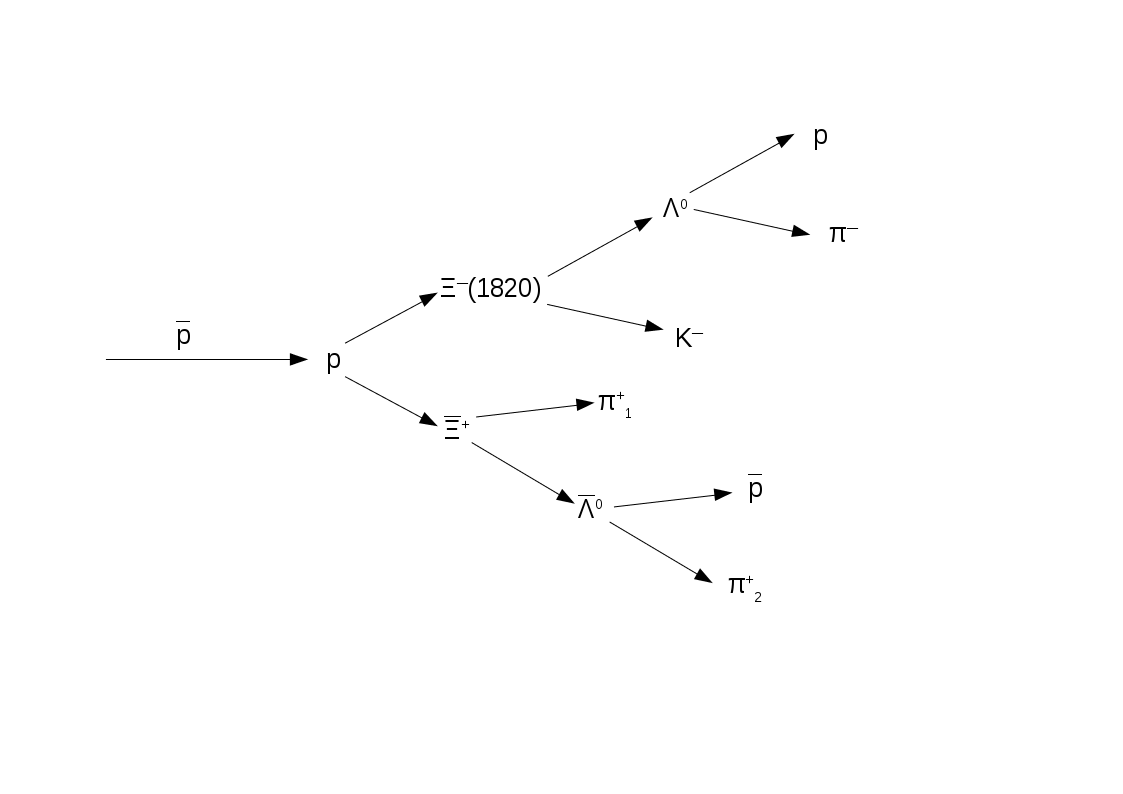
\includegraphics[width=1.00\textwidth]{./plots/DecayChannelXi1820.png}
	\caption{Simulated decay channel}
	\label{fig:eventgeneration_decaychannel}
\end{figure}

For the charge conjugated channel another 1.5 million events were generated.
Table \ref{tab:eventgeneration_parameter} shows the parameters which are used for the event generation.

\begin{table}[tbp]
	\caption{Parameter for event generation}
	\label{tab:eventgeneration_parameter}
	\centering
	\begin{tabular}{ll}
		\hline
		Parameter & Value \\
		\hline
		\hline
		Beam momentum & 4.6 \massunit \\
		Production & PHSP \\
		Tracking & Ideal \\
		Particle ID & Ideal \\\hline
		 
	\end{tabular}
\end{table}

The PHPS model is used for the production, because other models are not tested yet. 
But this is not effecting the strategy for this study.

The chosen beam momentum of $p_{\bar{\mt{p}}} = 4.6\unit{GeV/c}$ is 100 MeV above the production threshold of \excitedcascade and \anticascade.
The production cross section is expected to be of the same order ($\sim \mu\mt{b}$) as for \cascade \cite{PANDAphysics2009}.\\
\vspace{11pt} 

The used software versions for PandaRoot and the external software package is listed in table \ref{tab:eventgeneration_software} 

\begin{table}[tb]
	\centering
	\caption{Used software versions}
	\label{tab:eventgeneration_software}
	\begin{tabular}{ll}
		\hline
		Software & Version \\
		\hline
		\hline
		FairSoft & mar15\\
		FairRoot & v-15.03a \\
		PandaRoot & trunk revision 28555 \\
		Geant & 3\\
		Genfit & 1\\\hline
			 
	\end{tabular}
\end{table}


Since now \excitedcascade was not defined in the evt.pdl file. 
How the particle is added to the file is shown in the code snippet \ref{lst:eventgeneration_evtpdl}.
The properties of \excitedcascade are listed in table \ref{tab:eventgeneration_Xivalues}.

\begin{lstlisting}[caption={snippet from evt.pdl}\label{lst:eventgeneration_evtpdl}, captionpos=t,breaklines=true]
add  p Particle Xi(1820)- 23314 1.8230000e+00 2.4000000e-02 2.0000000e-01 -3 3 0.0000000e+00 23314
add  p Particle anti-Xi(1820)+ -23314 1.8230000e+00 2.4000000e-02 2.0000000e-01 3 3 0.0000000e+00 -23314
\end{lstlisting}

\begin{table}[htbp]
	\centering
	\caption{Properties of \excitedcascade and \excitedanticascade. The values are taken from \cite{PDG}}
	\label{tab:eventgeneration_Xivalues}
	\begin{tabular}{lllllll}
		\hline
		Particle & J & I & P & Charge & Mass  & Width \\
		\hline
		\hline
		&&&&&&\\
		\excitedcascade & $\frac{3}{2}$ & $\frac{1}{2}$ & ($-1$) & ($-1$) & ($1.823 \pm 5$)\massunit & ($0.024 \pm 6) $ GeV \\
		\excitedanticascade & $\frac{3}{2}$ & $\frac{1}{2}$ & ($-1$) & 1 & ($1.823 \pm 5$)\massunit & ($0.024 \pm 6) $ GeV\\
		\hline
		  
	\end{tabular}
\end{table}

The generated transverse momentum against the longitudinal momentum for \lam, \alam, \anticascade and \excitedcascade is 
presented in figure \ref{fig:MC_lambda0_pt_vs_pz}% -- \ref{fig:MC_xi_pt_vs_pz}.\\


\begin{figure}
	\subfigure[\lam]{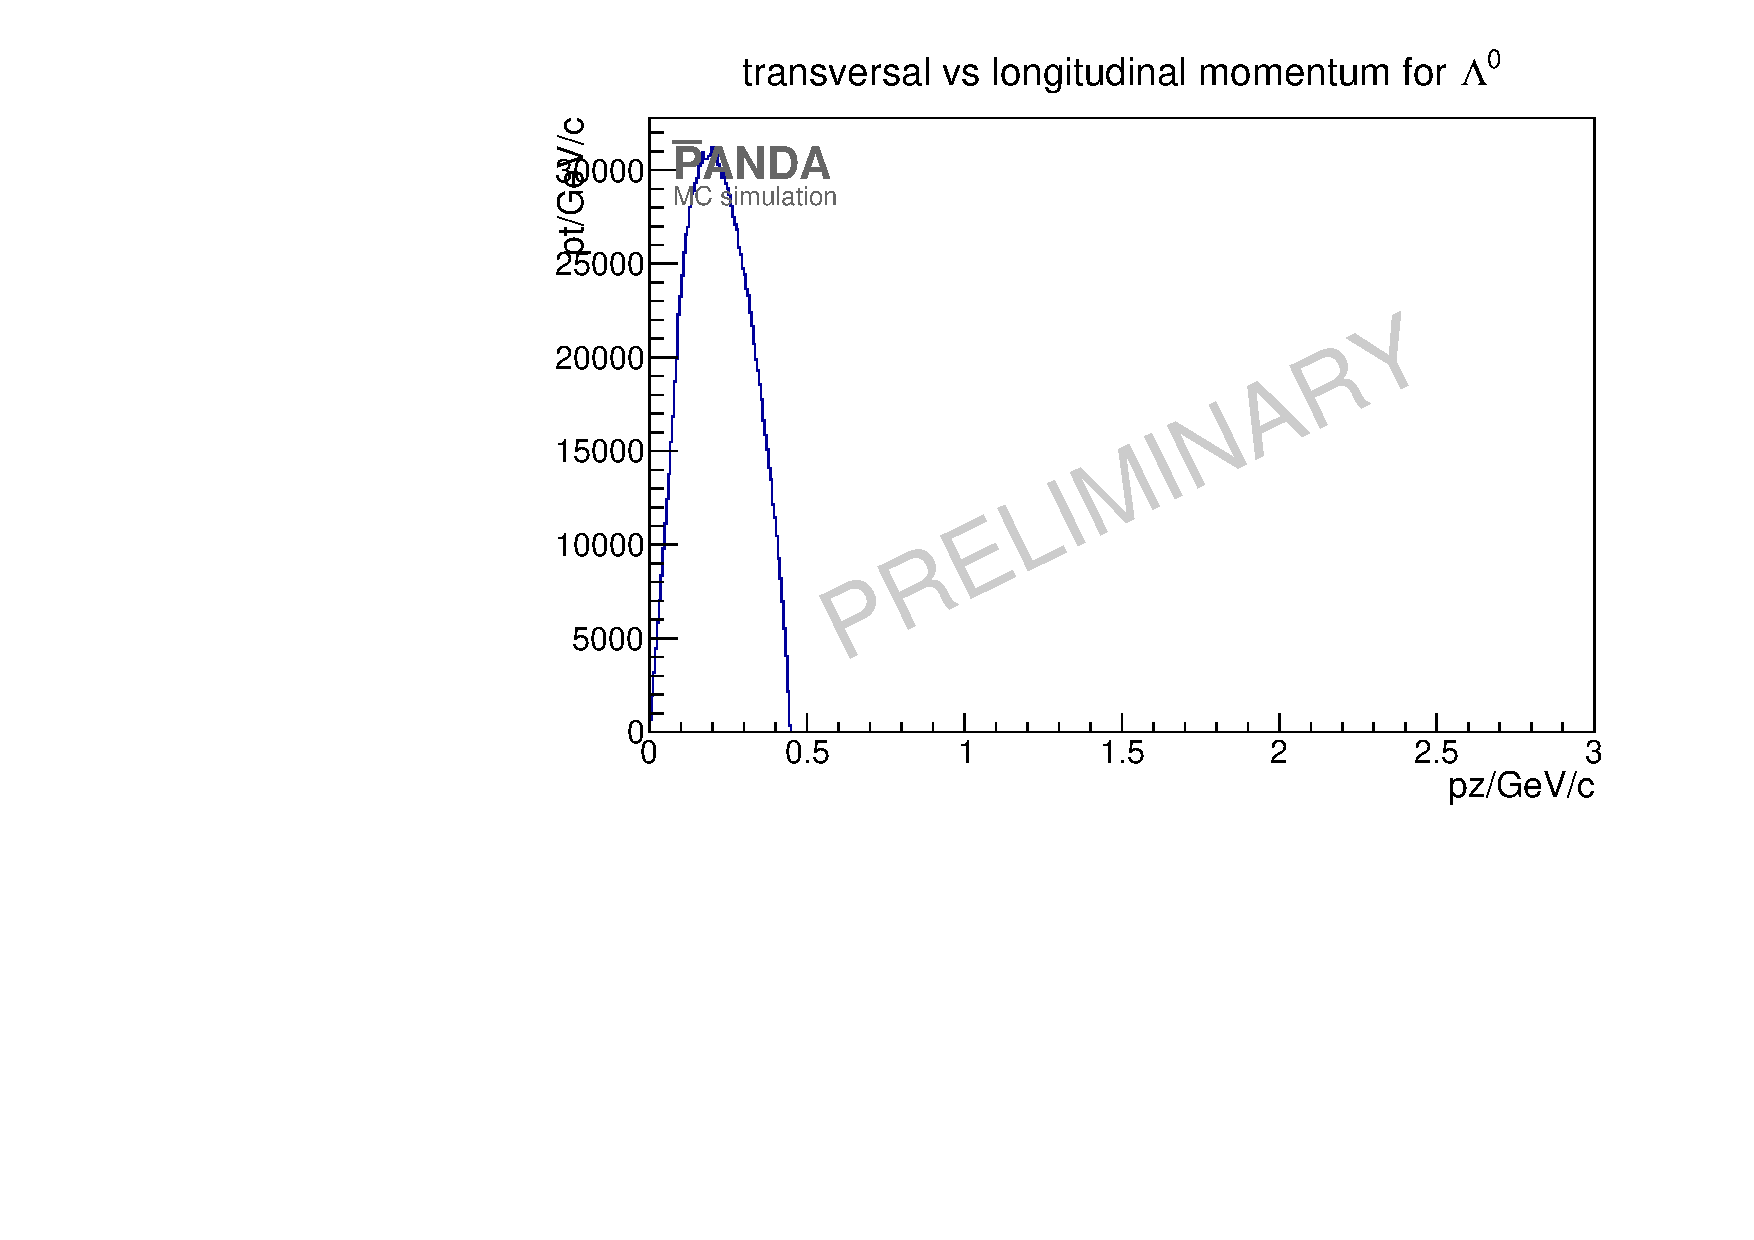
\includegraphics[width=0.49\textwidth]{./plots/lambda0/Lambda0_MC_pt_vs_pz.pdf}}
	\subfigure[\alam]{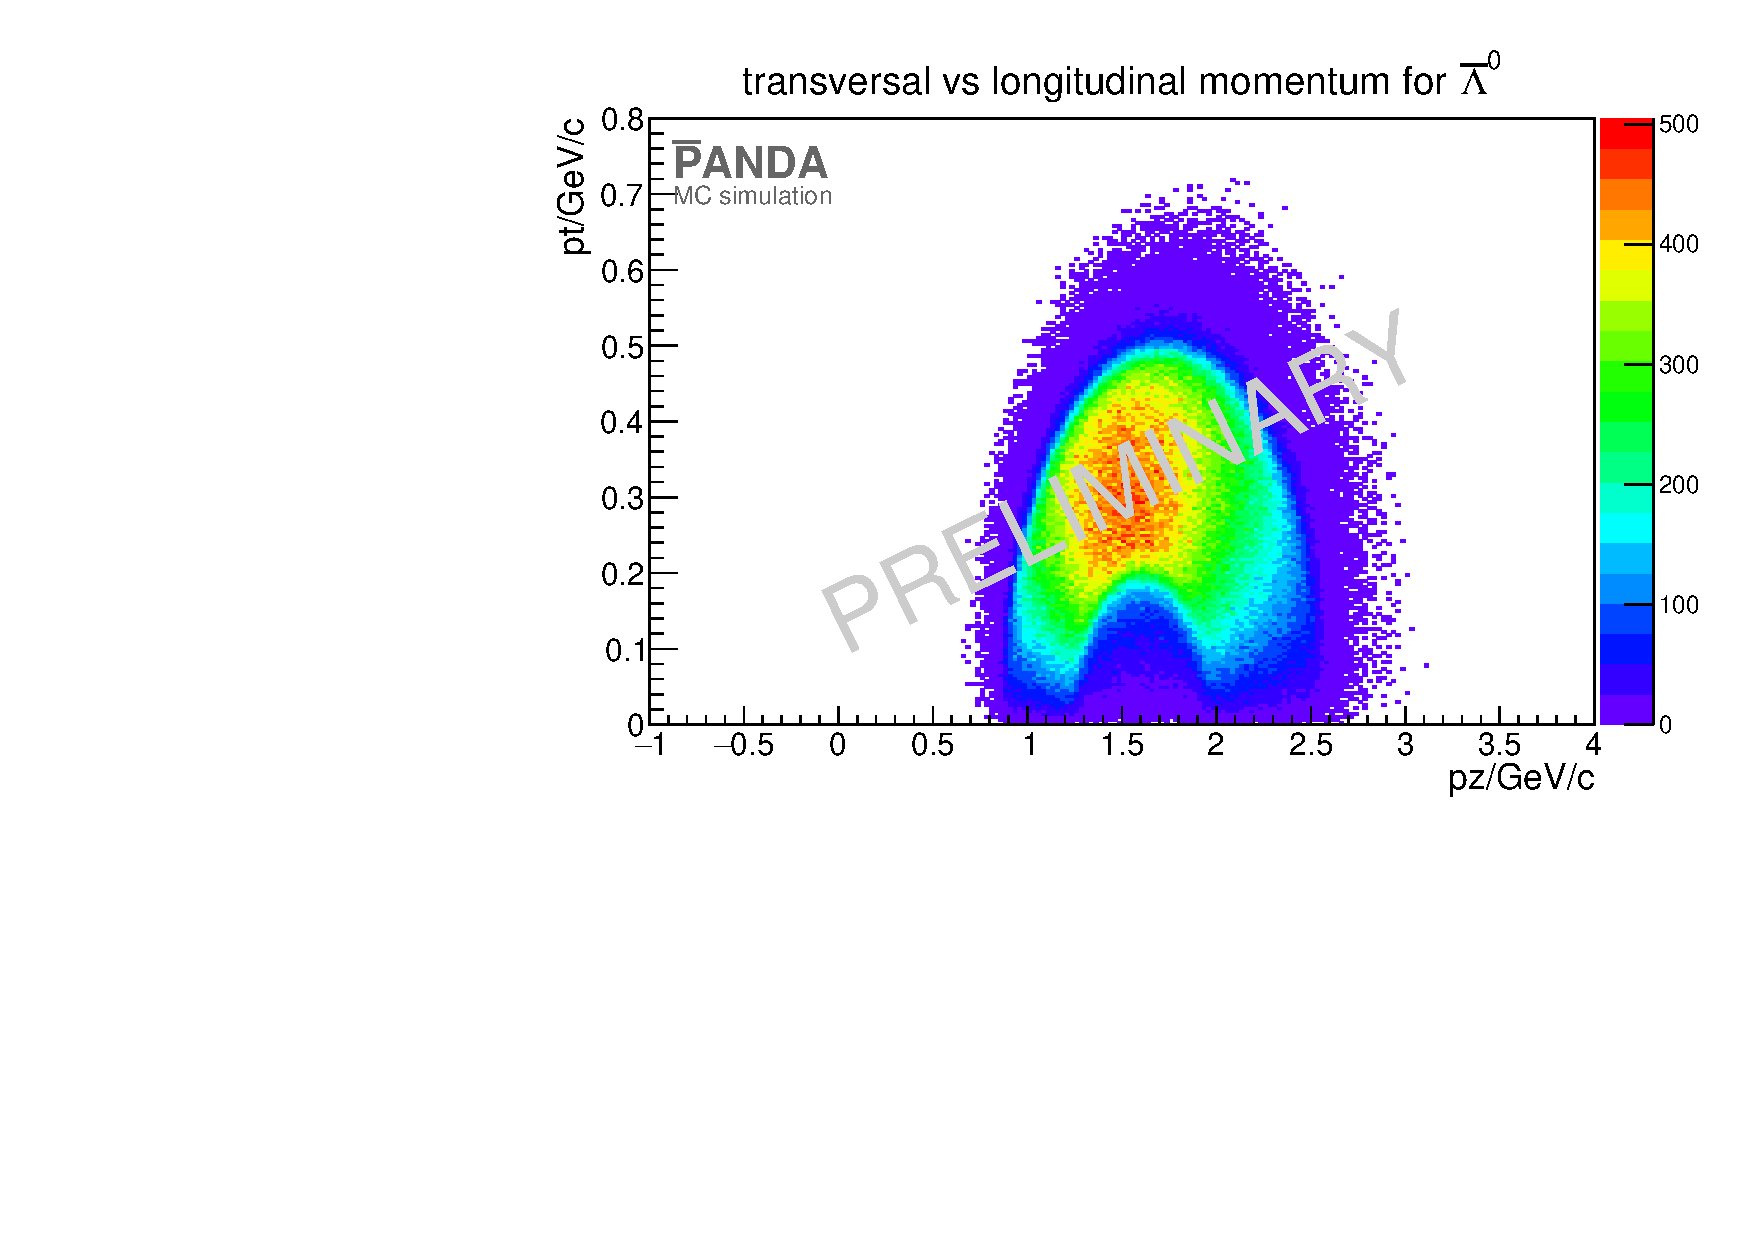
\includegraphics[width=0.49\textwidth]{./plots/antilambda0/AntiLambda0_MC_pt_vs_pz.pdf}}
	\caption{\propose Figure a) shows the transverse momentum on the y axis against the longitudinal momentum on the x axis for \lam. Figure b) 
			shows the same distribution for \alam.}
	\label{fig:MC_lambda0_pt_vs_pz}
\end{figure}


\begin{figure}
	\subfigure[\anticascade]{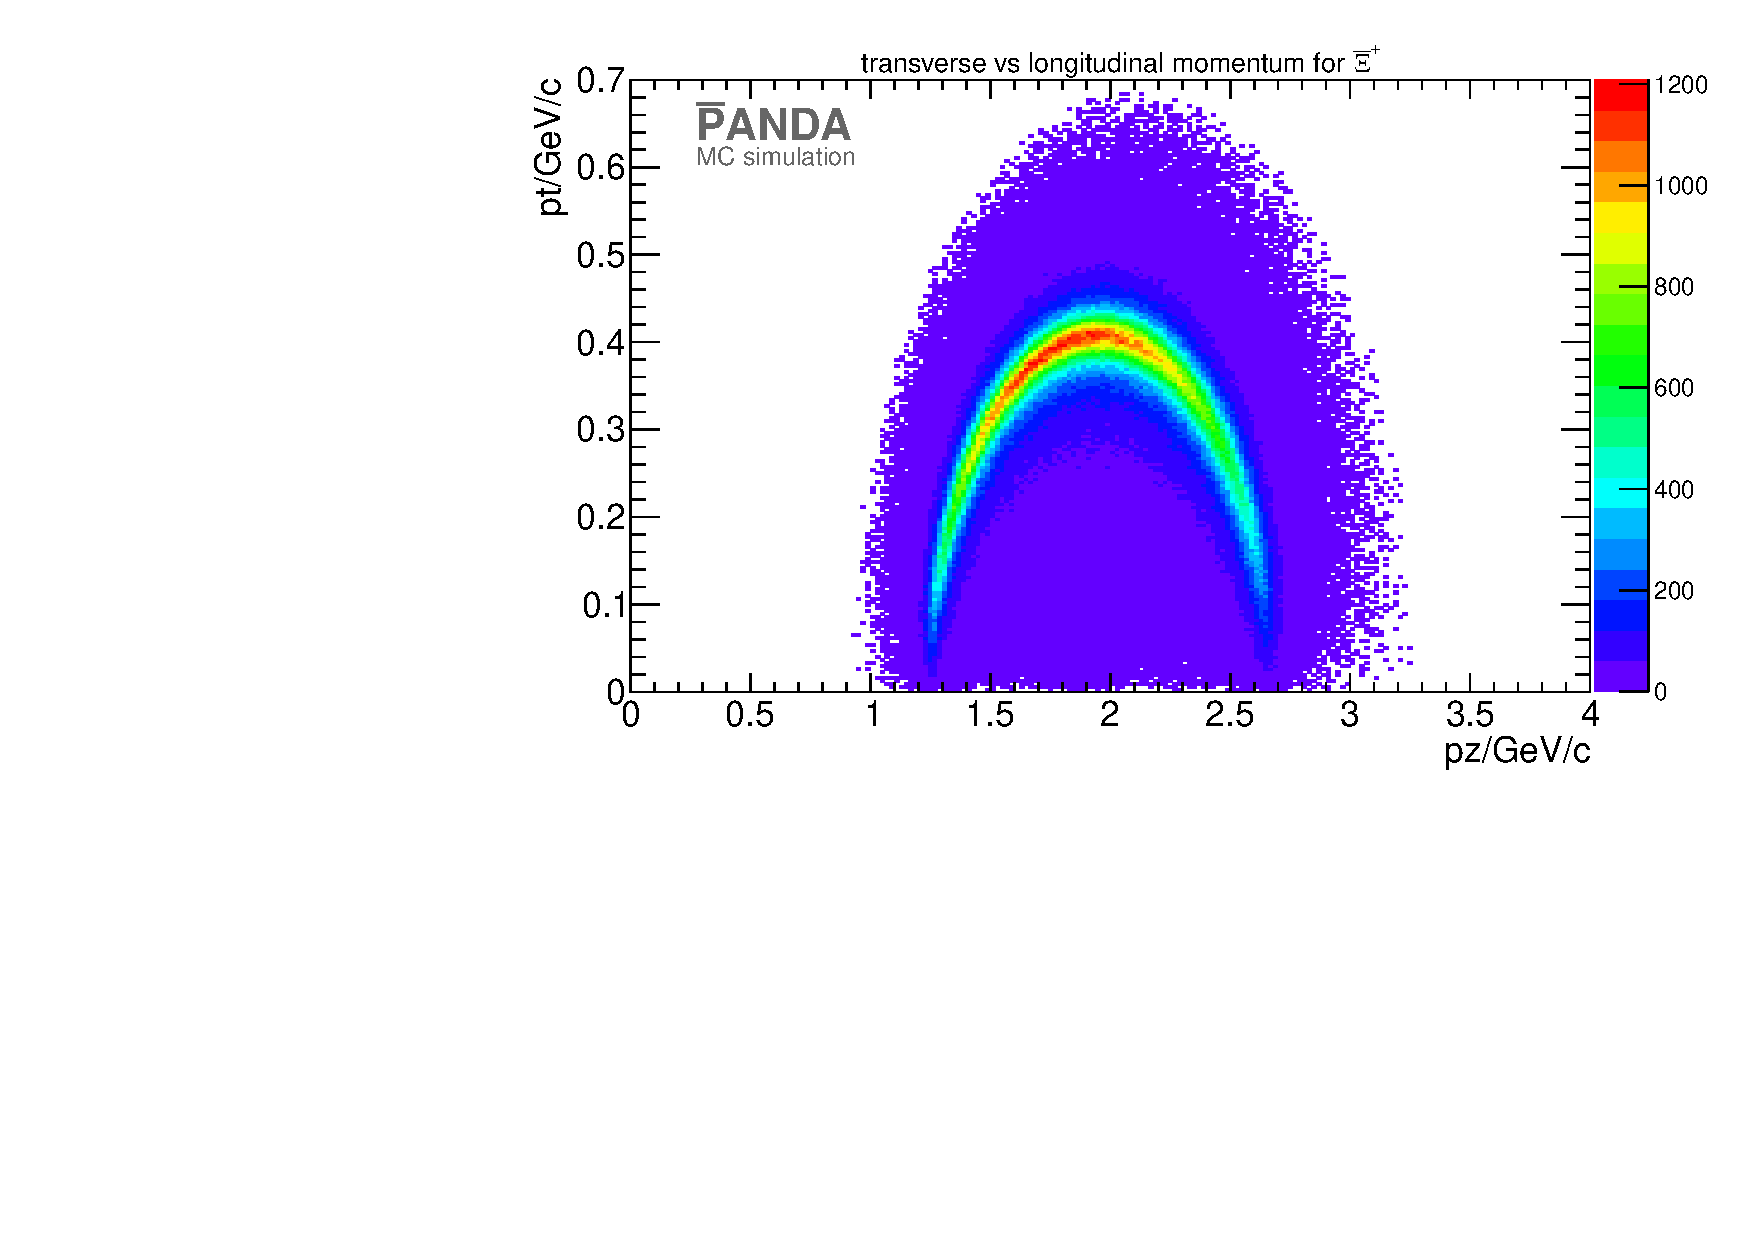
\includegraphics[width=0.49\textwidth]{./plots/Xi/XiPlus_MC_pt_vs_pz.pdf}}
	\subfigure[\excitedcascade]{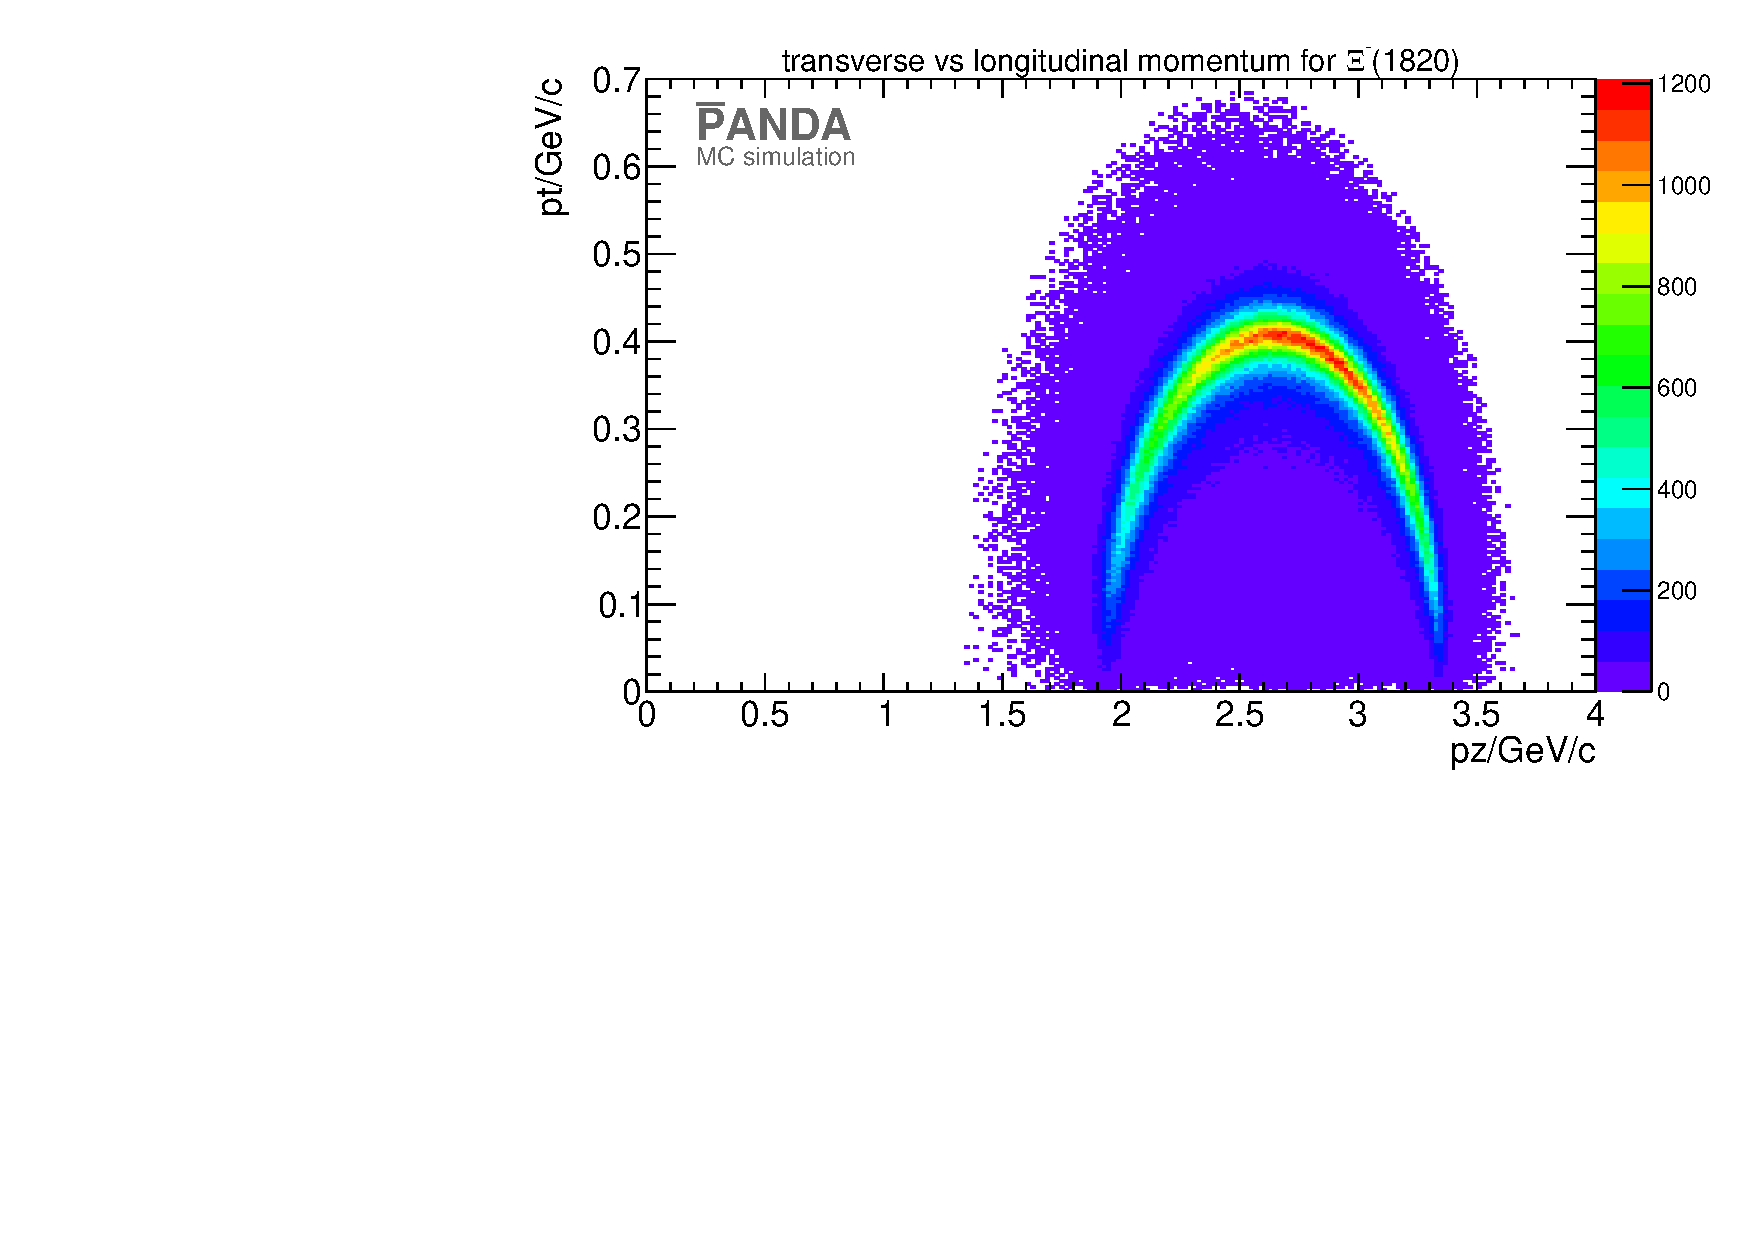
\includegraphics[width=0.49\textwidth]{./plots/Xi1820/XiMinus1820_MC_pt_vs_pz.pdf}}
	\caption{\propose Figure a) shows transverse against the longitudinal momentum distribution for \anticascade. Figure b) 
			transverse versus longitudinal momentum distribution for \excitedcascade.}
	\label{fig:MC_xi_pt_vs_pz}
\end{figure}

Figure \ref{fig:eventgeneration_Dalitz} shows the Dalitz plot for the \lam, \kminus and \anticascade final states for 
the channel \pbarpSystem $\rightarrow$ \excitedcascade \anticascade. 

\begin{figure}
	\centering
	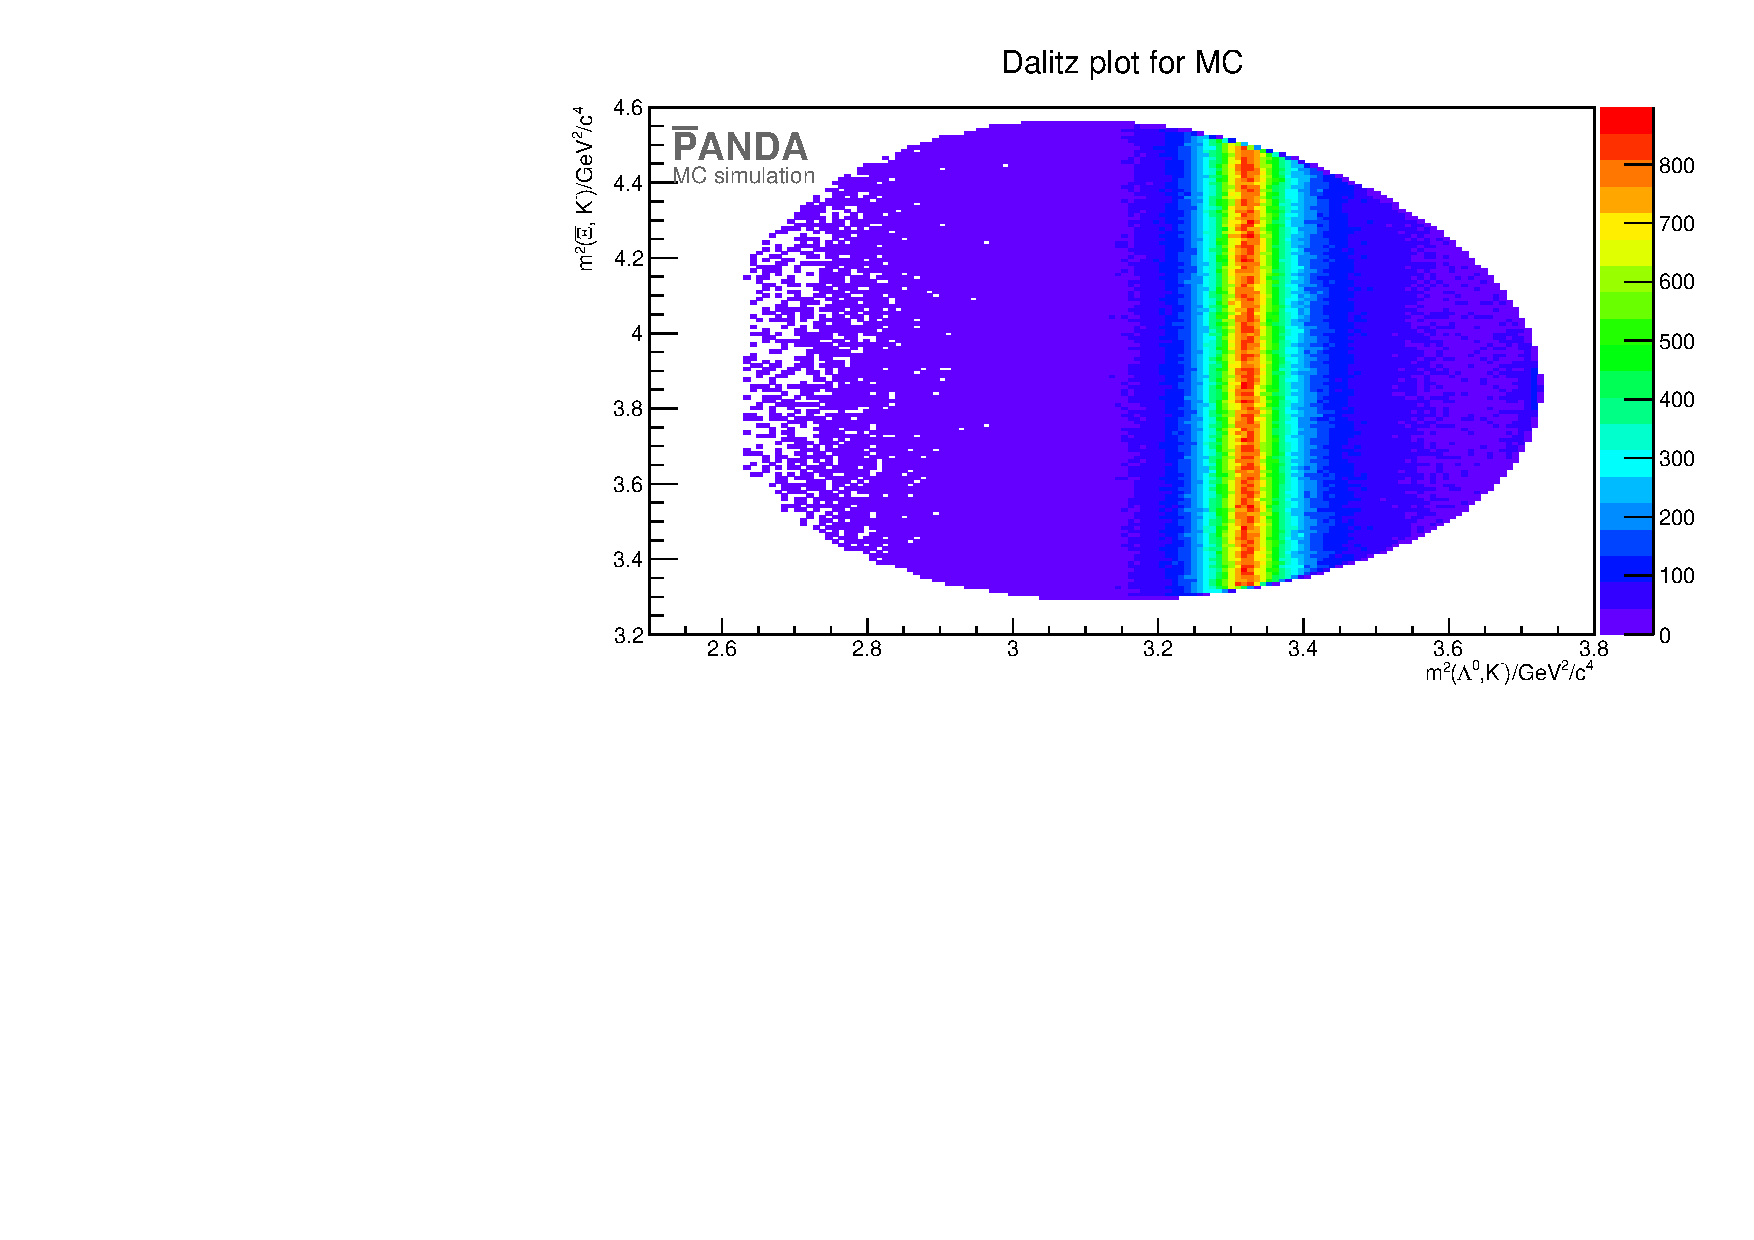
\includegraphics[width=0.6\textwidth]{./plots/Dalitzplot_MC.pdf}
	\caption{\propose Dalitz plot for simulation. On x axis is the mass square of \lam  and \kminus and on the y axis there is the mass square of \anticascade and \kminus}
	\label{fig:eventgeneration_Dalitz}
\end{figure}


	
	\chapter{Analysis}
		To reconstruct all the simulated particles we start with the final state particles and go backwards through the reaction chain.

\section{Final state particle}
	The selected final state particle are protons, antiproton, \piminus, \piplus, \kminus and \kplus mesons.
	For the reconstruction of these final state particles I used an ideal tracking. 
	To make the selection a bit more realistic only particles with more than 3 hits in any inner tracking detector (MVD, STT and GEM)
	are selected.
	The selection criterion is chosen because three hits are defining a circle.
	A fourth hit point is than a validation of the track hypothesis.\\
	The particle identification (PID) is also ideal. 
	The selection criterion is set to 'best'.\vspace{11pt} \\
	The reconstruction  efficiency for the final state particle is shown in table \ref{tab:finalstate_recoeff} and figure \ref{fig:finalstate_recoeff}.
	
	\begin{table}
		\centering
		\caption{\propose reco efficiency and momentum resolution for \pbarpSystem $\rightarrow$ \excitedcascade \anticascade}
		\label{tab:finalstate_recoeff}
		\begin{tabular}{lll}
			\hline
			final state & N/$\%$ & $\frac{\sigma p}{p}/\%$ \\
			\hline
			\hline
			\piminus & 83.48 & 1.53\\
			\piplusone(\anticascade) &  80.93& 1.38 \\
			\piplustwo(\alam) &  83.07& 1.49\\
			\kminus&  78.59& 1.58\\
			p &  84.39& 1.61\\
			\antiproton & 78.25 & 1.61\\\hline
			 
		\end{tabular}
	\end{table}
	
	Table \ref{tab:finalstate_recoeff_cc} shows the reconstruction efficiency for the c.c. channel.
	
	\begin{table}
		\centering
		\caption{\propose reco efficiency and momentum resolution for \pbarpSystem $\rightarrow$ \excitedanticascade \cascade}
		\label{tab:finalstate_recoeff_cc}
		\begin{tabular}{lll}
			\hline
			final state & N/$\%$ & $\frac{\sigma p}{p}/\%$ \\
			\hline
			\hline
			\piplus &  82.9625&   1.54131\\
			\piminusone(\cascade) & 80.395&   1.37697  \\
			\piminustwo(\lam) &  82.6867&   1.48918\\
			\kplus& 83.2709&   1.57882 \\
			p &  80.7079&   1.55197\\
			\antiproton &  80.9253&   1.60091\\\hline
			 
		\end{tabular}
	\end{table}
	
	\begin{figure}
	
		\centering
		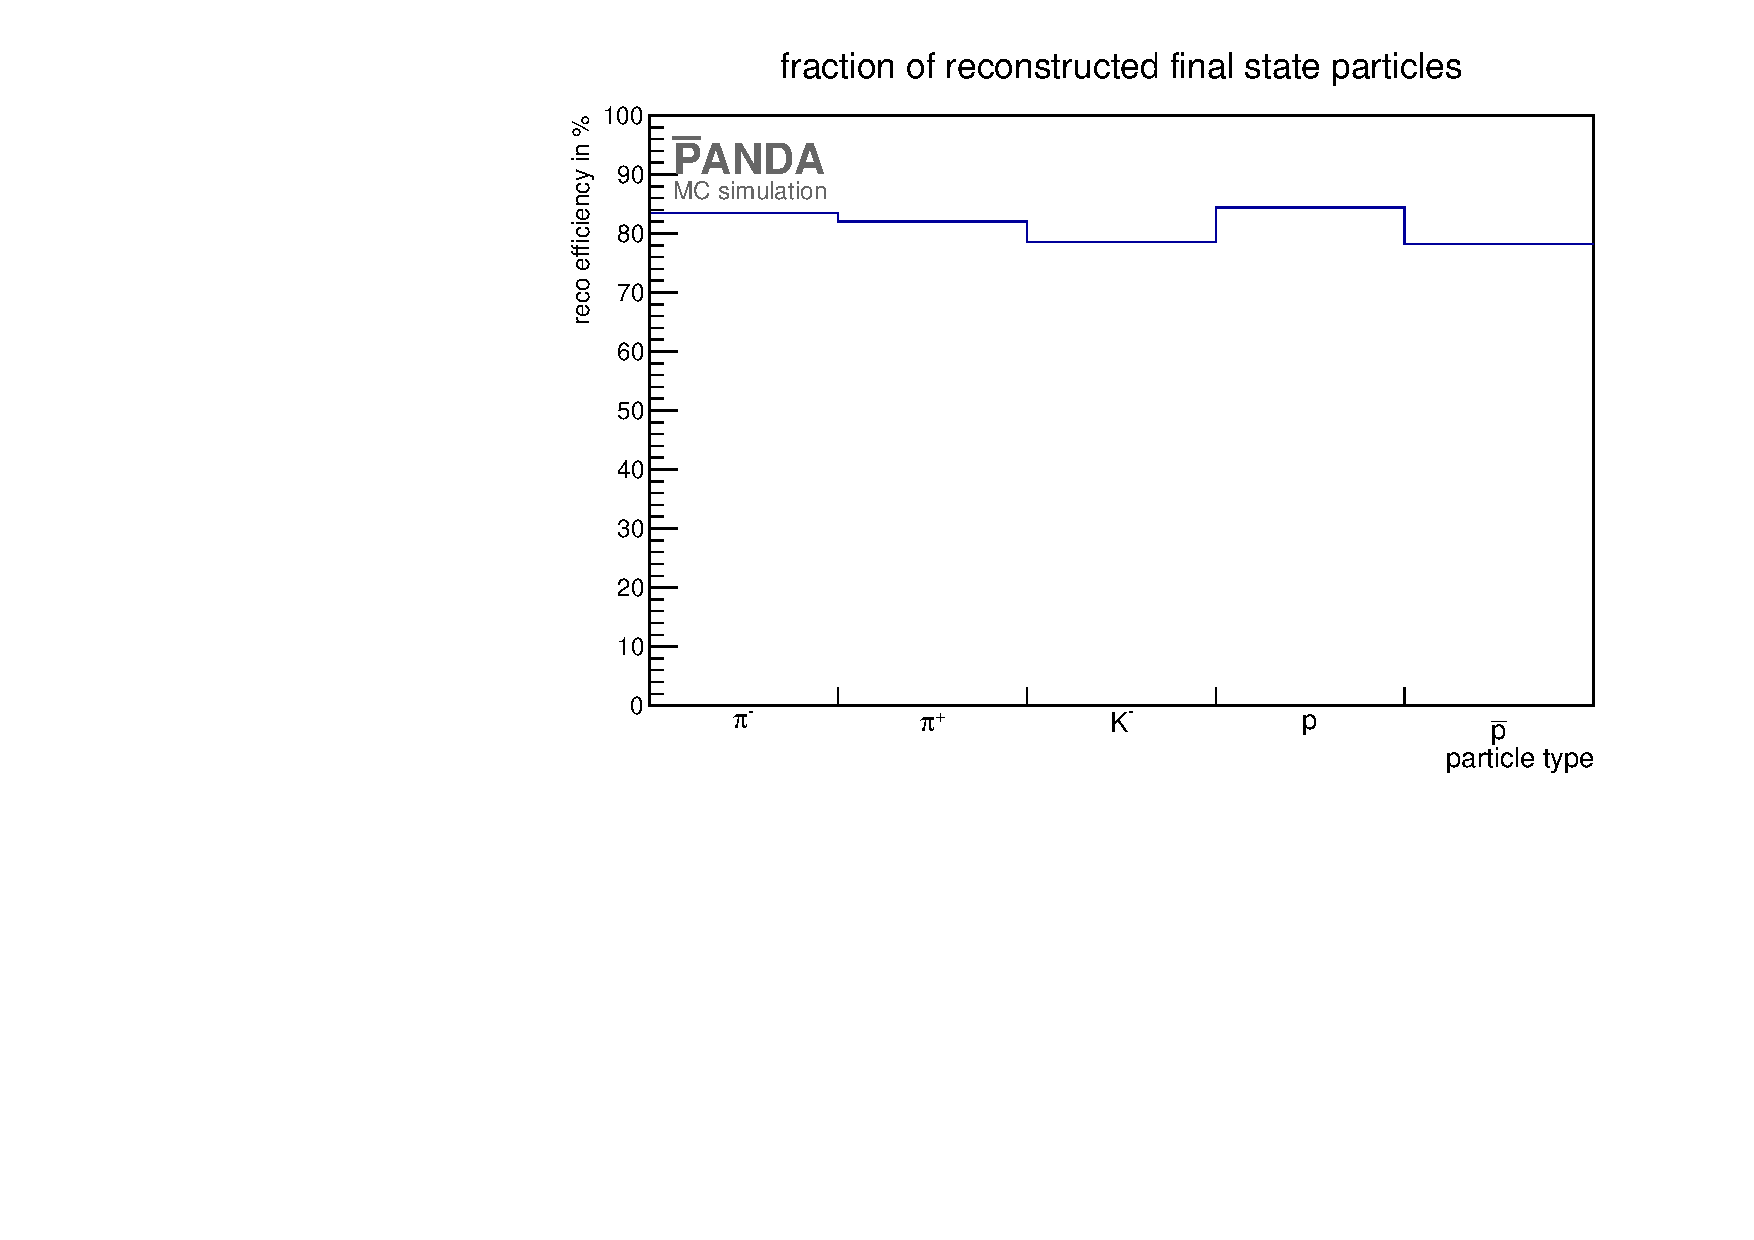
\includegraphics[width=0.8\textwidth]{./plots/finalstate/reco_efficiency.pdf}
		\caption{\propose Reconstruction efficiency for final state particles. The x axis shows the particle type. 
				On the y axis is shown the fraction of reconstructed particles, like it is shown in table \ref{tab:finalstate_recoeff}}
		\label{fig:finalstate_recoeff}
	
	\end{figure}
	

	
\section{Reconstruction of $\Lambda^0$ and $\bar{\Lambda}^0$}
	\subsection*{Selection}
		For the reconstruction of 
		
		\begin{itemize}
			\item \lam a proton and a \piminus meson are combined and
			\item for the reconstruction of \alam a \antiproton and a \piplus are combined.
		\end{itemize}
		 
		After the combination of the daughter particles a mass window cut is performed.
		Only those particles are chosen which have a mass within $0.3$\massunit.
		
		
		A vertex constraint fit with the PndKinVtxFitter is performed on the selected particle.
		This means that the tracks of the daughter particles are fitted to a common vertex point.  
		The \chisq and \chisq-Probability distribution of the vertex fit for \lam is shown in figure \ref{fig:lambda_chi2}.
		
		\begin{figure}
			\centering
				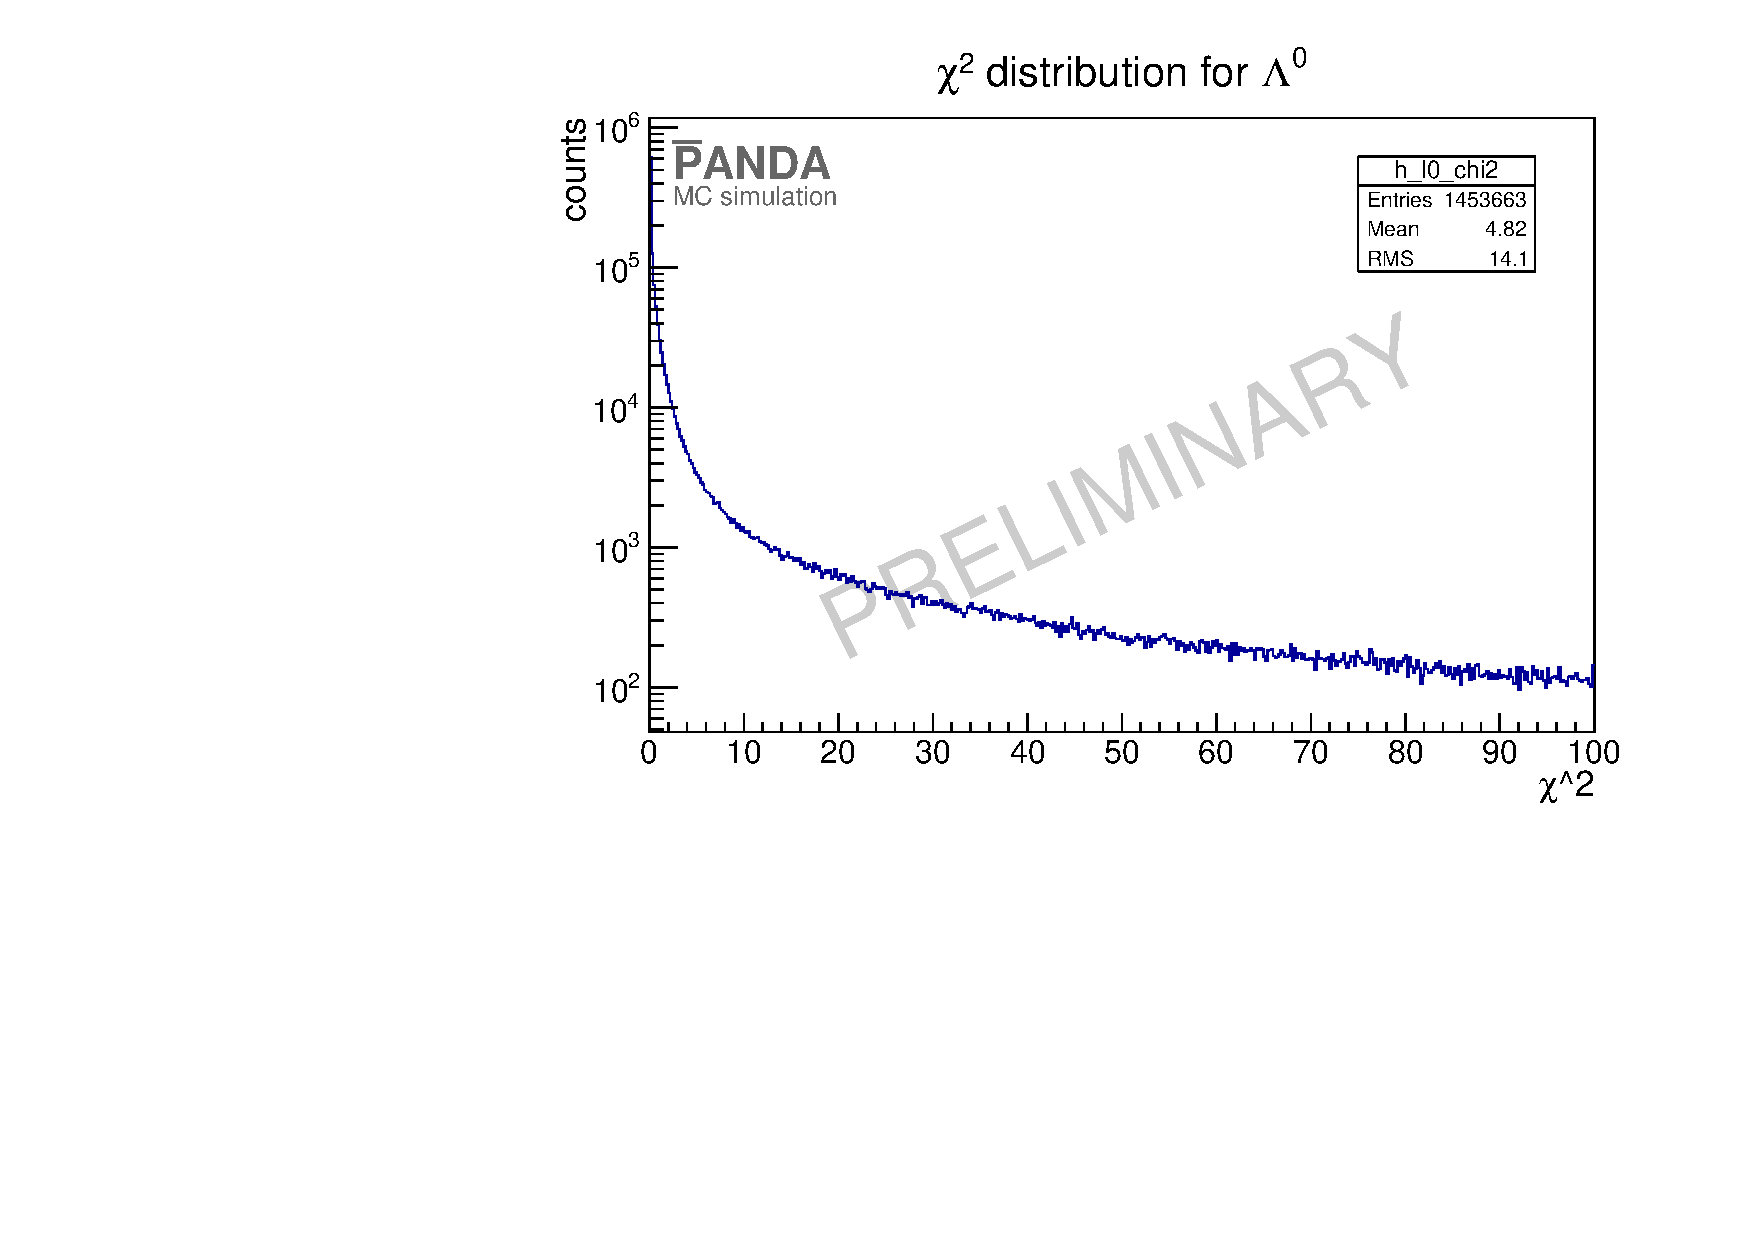
\includegraphics[width=0.50\textwidth]{./plots/lambda0/lambda0_chisqrt.pdf}
				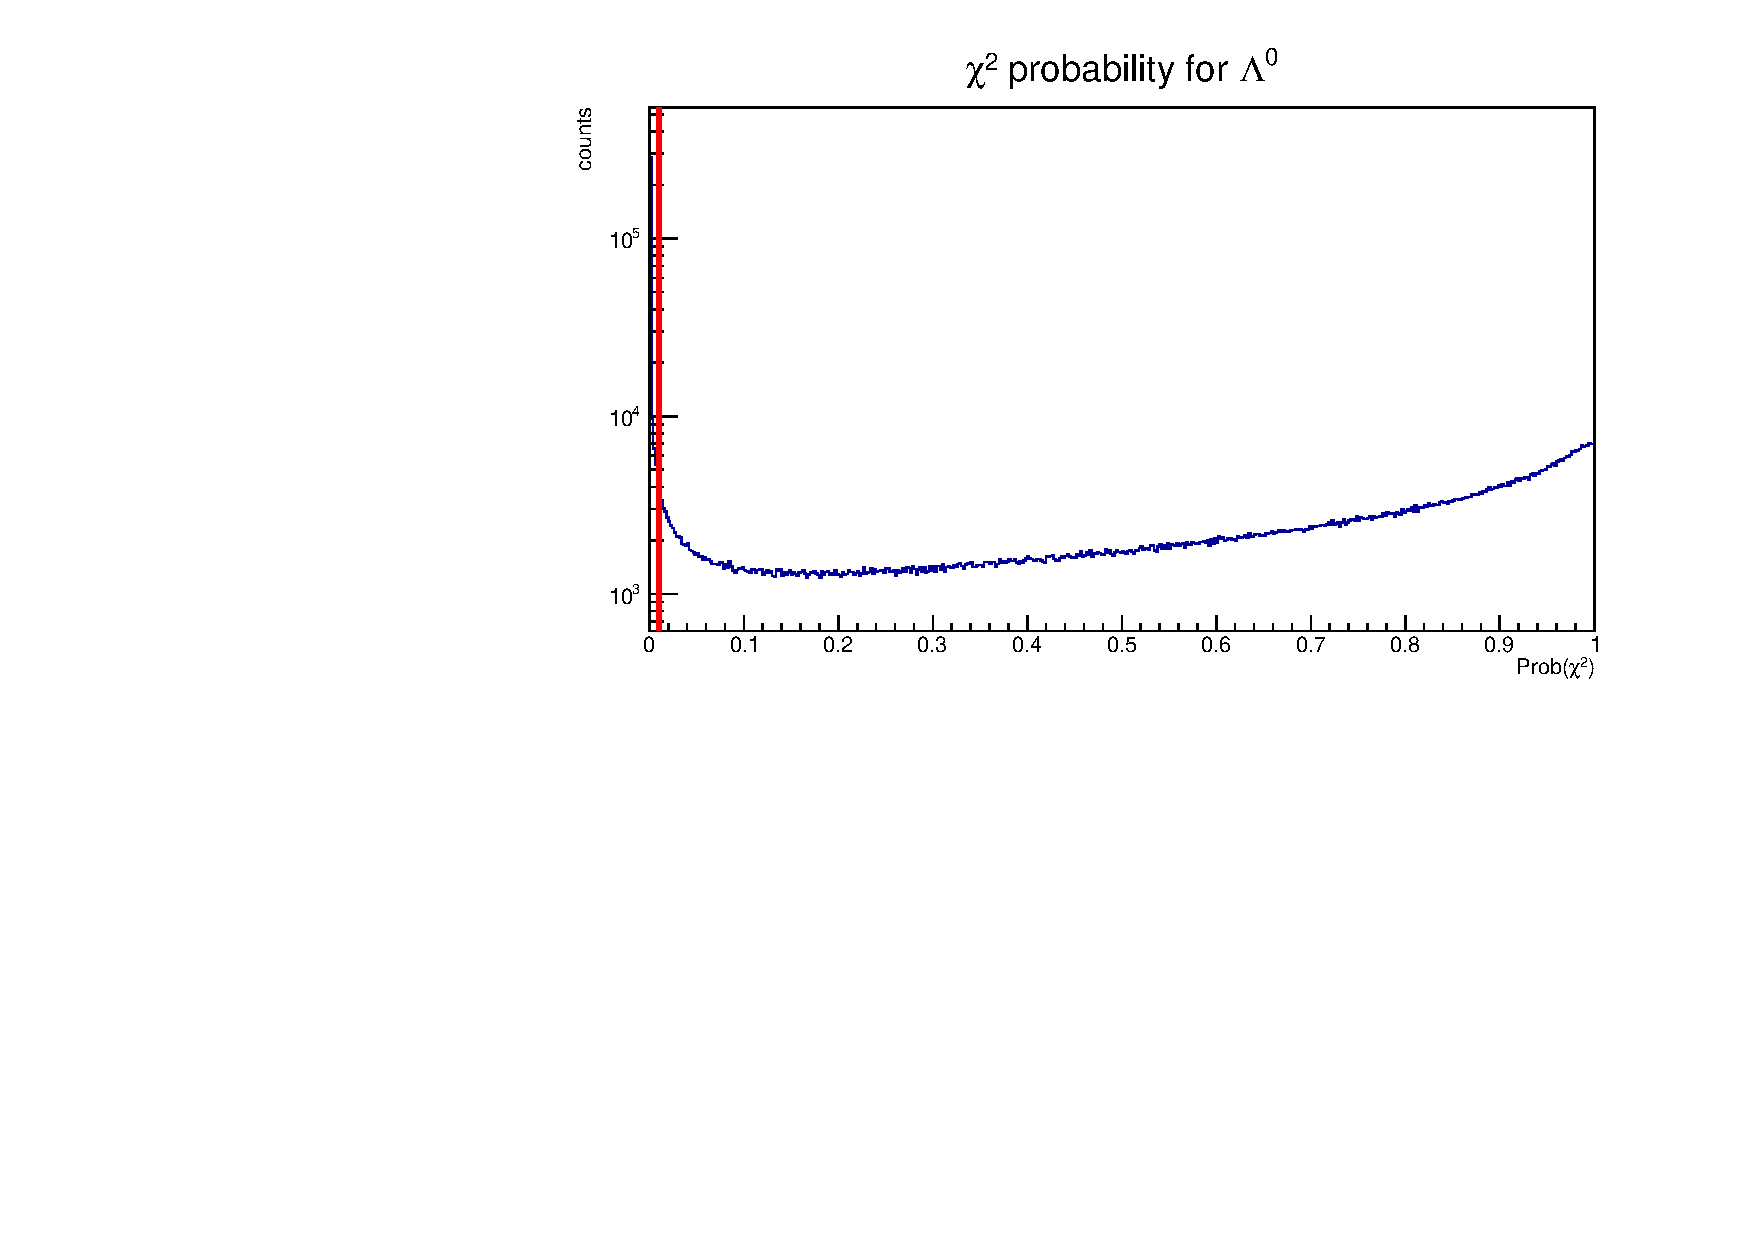
\includegraphics [width=0.50\textwidth]{./plots/lambda0/lambda0_prob.pdf}
			\caption{\propose upper: \chisq distribution; lower: \chisq probability distribution}
			\label{fig:lambda_chi2}
		\end{figure}
		
		In the \chisq-probability distribution one can see a increasing number of events for probabilities going to one.
		These feature is not coming from vertex fitting.
		There is still a problem with covariance matrices which causes the effect.
		\vspace{11pt}\\
		The fit information coming from the vertex fit are used to perform a mass constraint fit with the kinematic fitter PndKinFitter.
		After using both fitter the selection criterion is set. 
		One select only those particles which have a probability greater than $1\%$ in both fitter.
		A scheme which shows how the events are selected can be found in figure \ref{fig:lambda_scheme}. 
		
		\begin{figure}
			\centering
				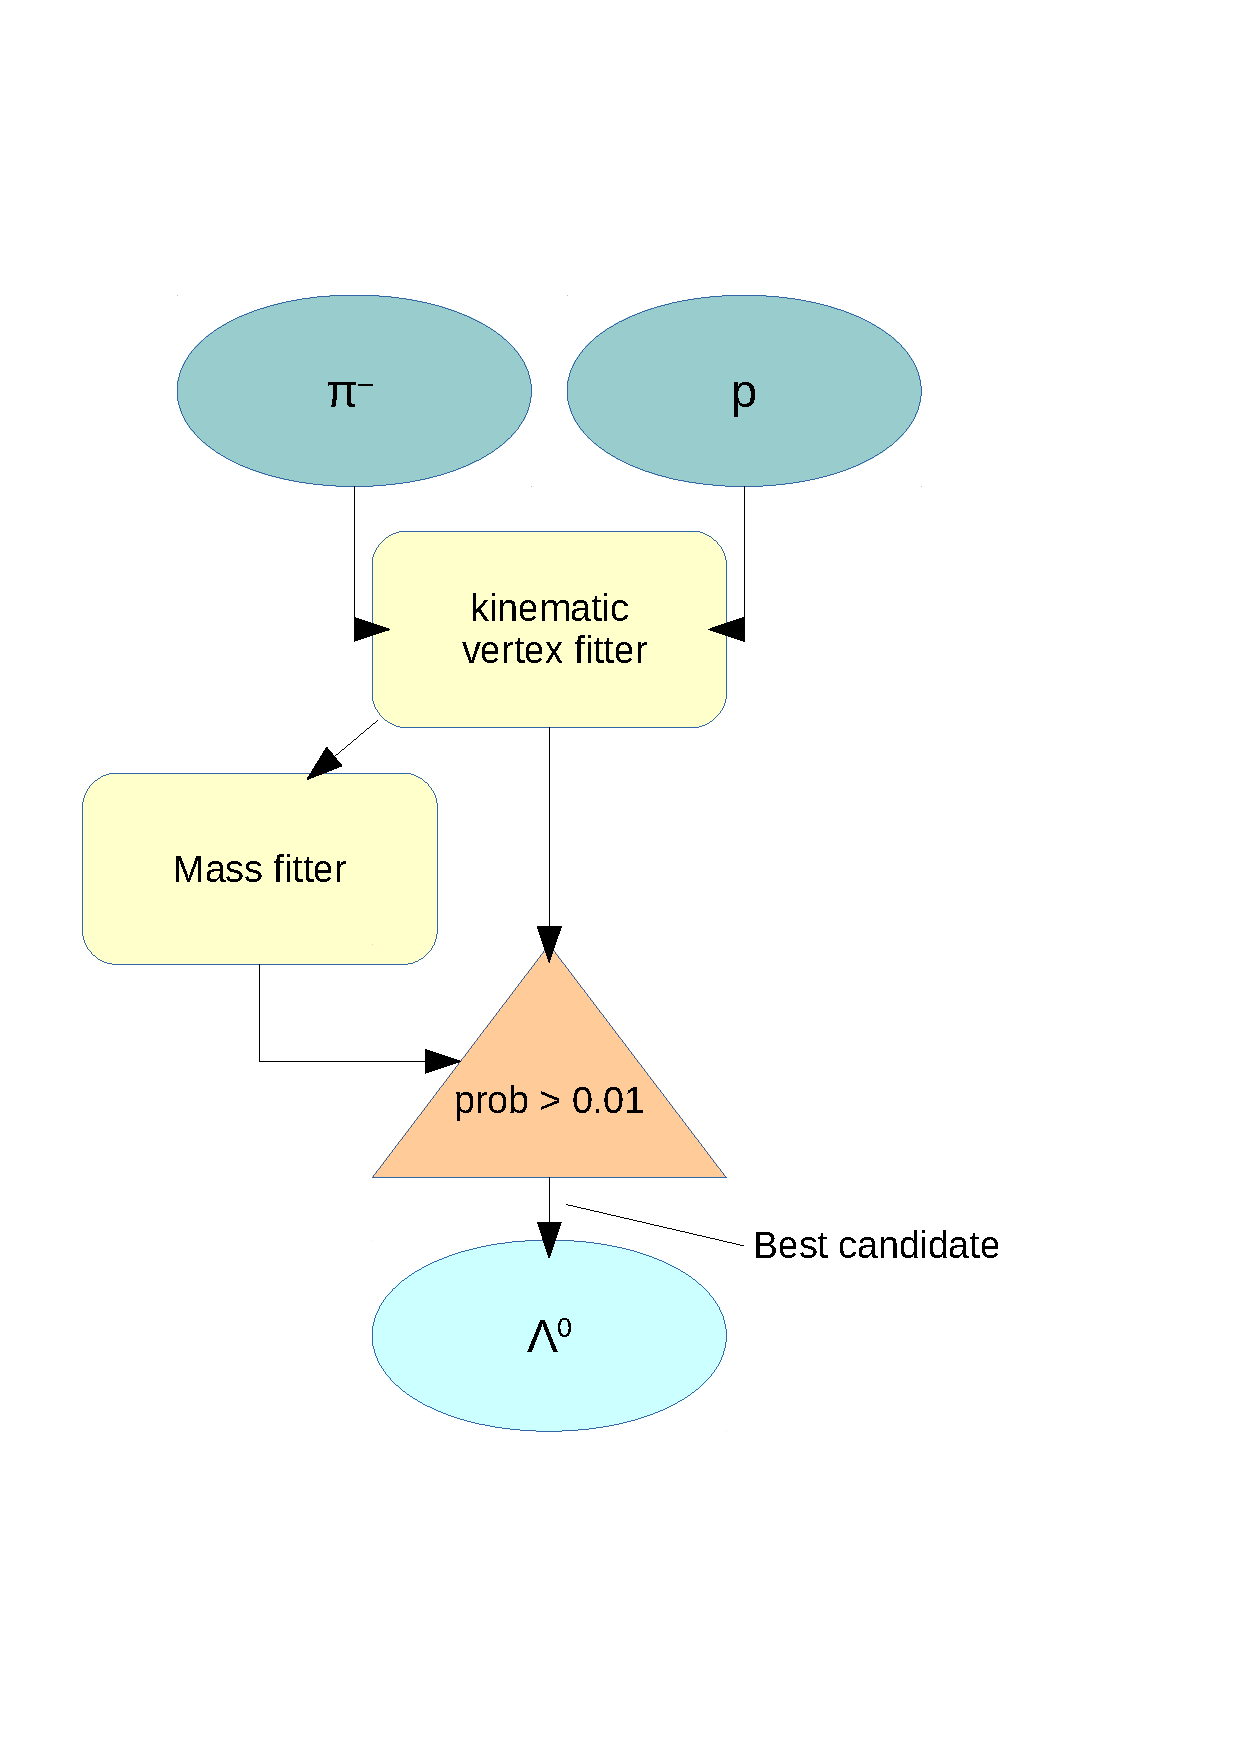
\includegraphics[width=0.50\textwidth]{./plots/combineLambda0.pdf}
			\caption{propose Scheme for \lam reconstruction}
			\label{fig:lambda_scheme}
		\end{figure}
		
		If there is more than one candidate left after the cuts the best fitted candidate is chosen.
		
		
	\subsection*{Results}
		This subsection presents the results for the \lam and \alam selection with the selection criteria introduced above.
		The mass distributions for different cuts are shown in figure \ref{fig:lambda0_massdiffcuts} and figure \ref{fig:antilambda0_massdiffcuts}.
	
		\begin{figure}
			\centering
				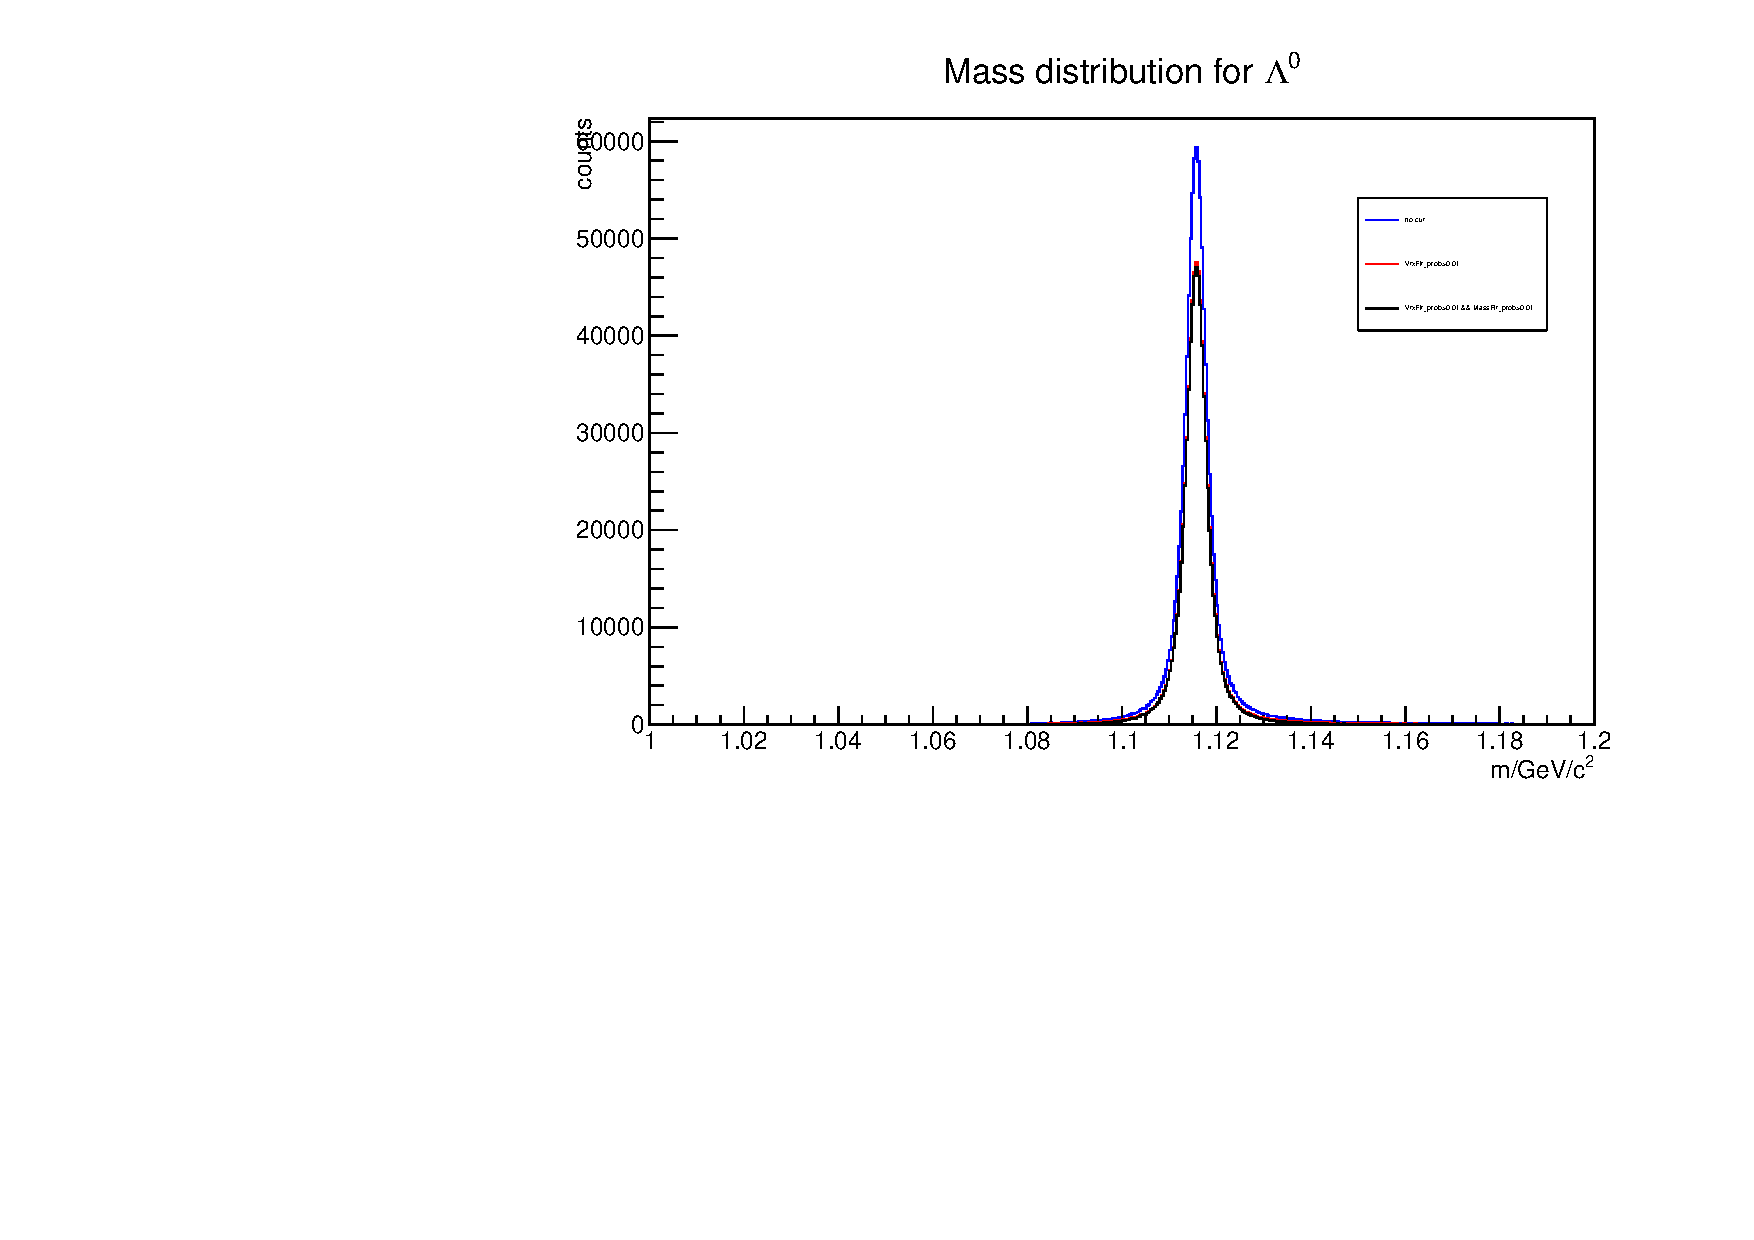
\includegraphics[width=1.1\textwidth]{./plots/lambda0/lambda0_m_diffcuts.pdf}
			\caption{\propose Mass distribution of \lam for different cuts}
			\label{fig:lambda0_massdiffcuts}
			
				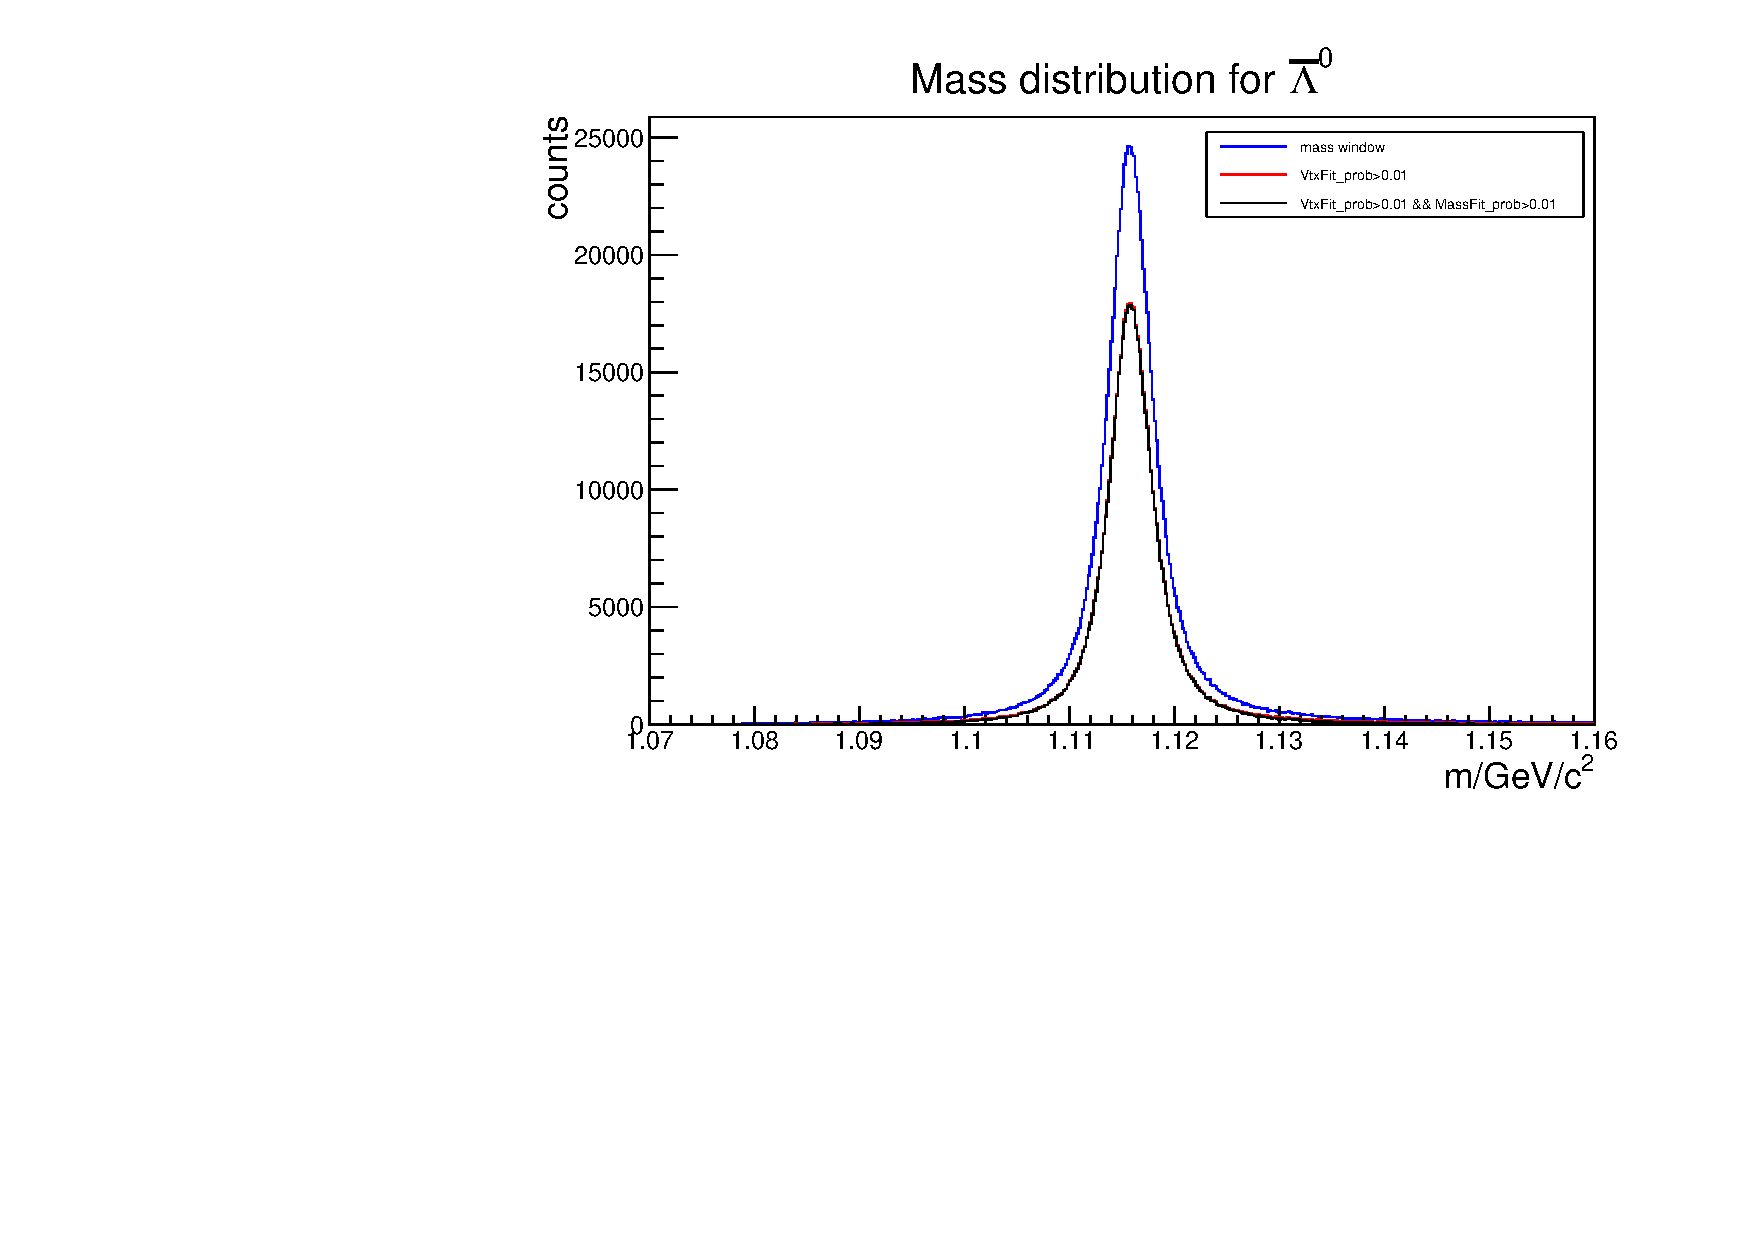
\includegraphics[width=1.1\textwidth]{./plots/antilambda0/antiLambda0_m_diffcuts.pdf}
			\caption{\propose Mass distribution of \alam for different cuts}
			\label{fig:antilambda0_massdiffcuts}
		\end{figure}
		
		The reconstructed mass can be derived by performing a double Gaussian fit on the cut mass.
		The mass distribution and the double Gaussian fit are exemplarily shown for \lam in figure \ref{fig:lambda0_massfit}
		
		\begin{figure}
			\centering
				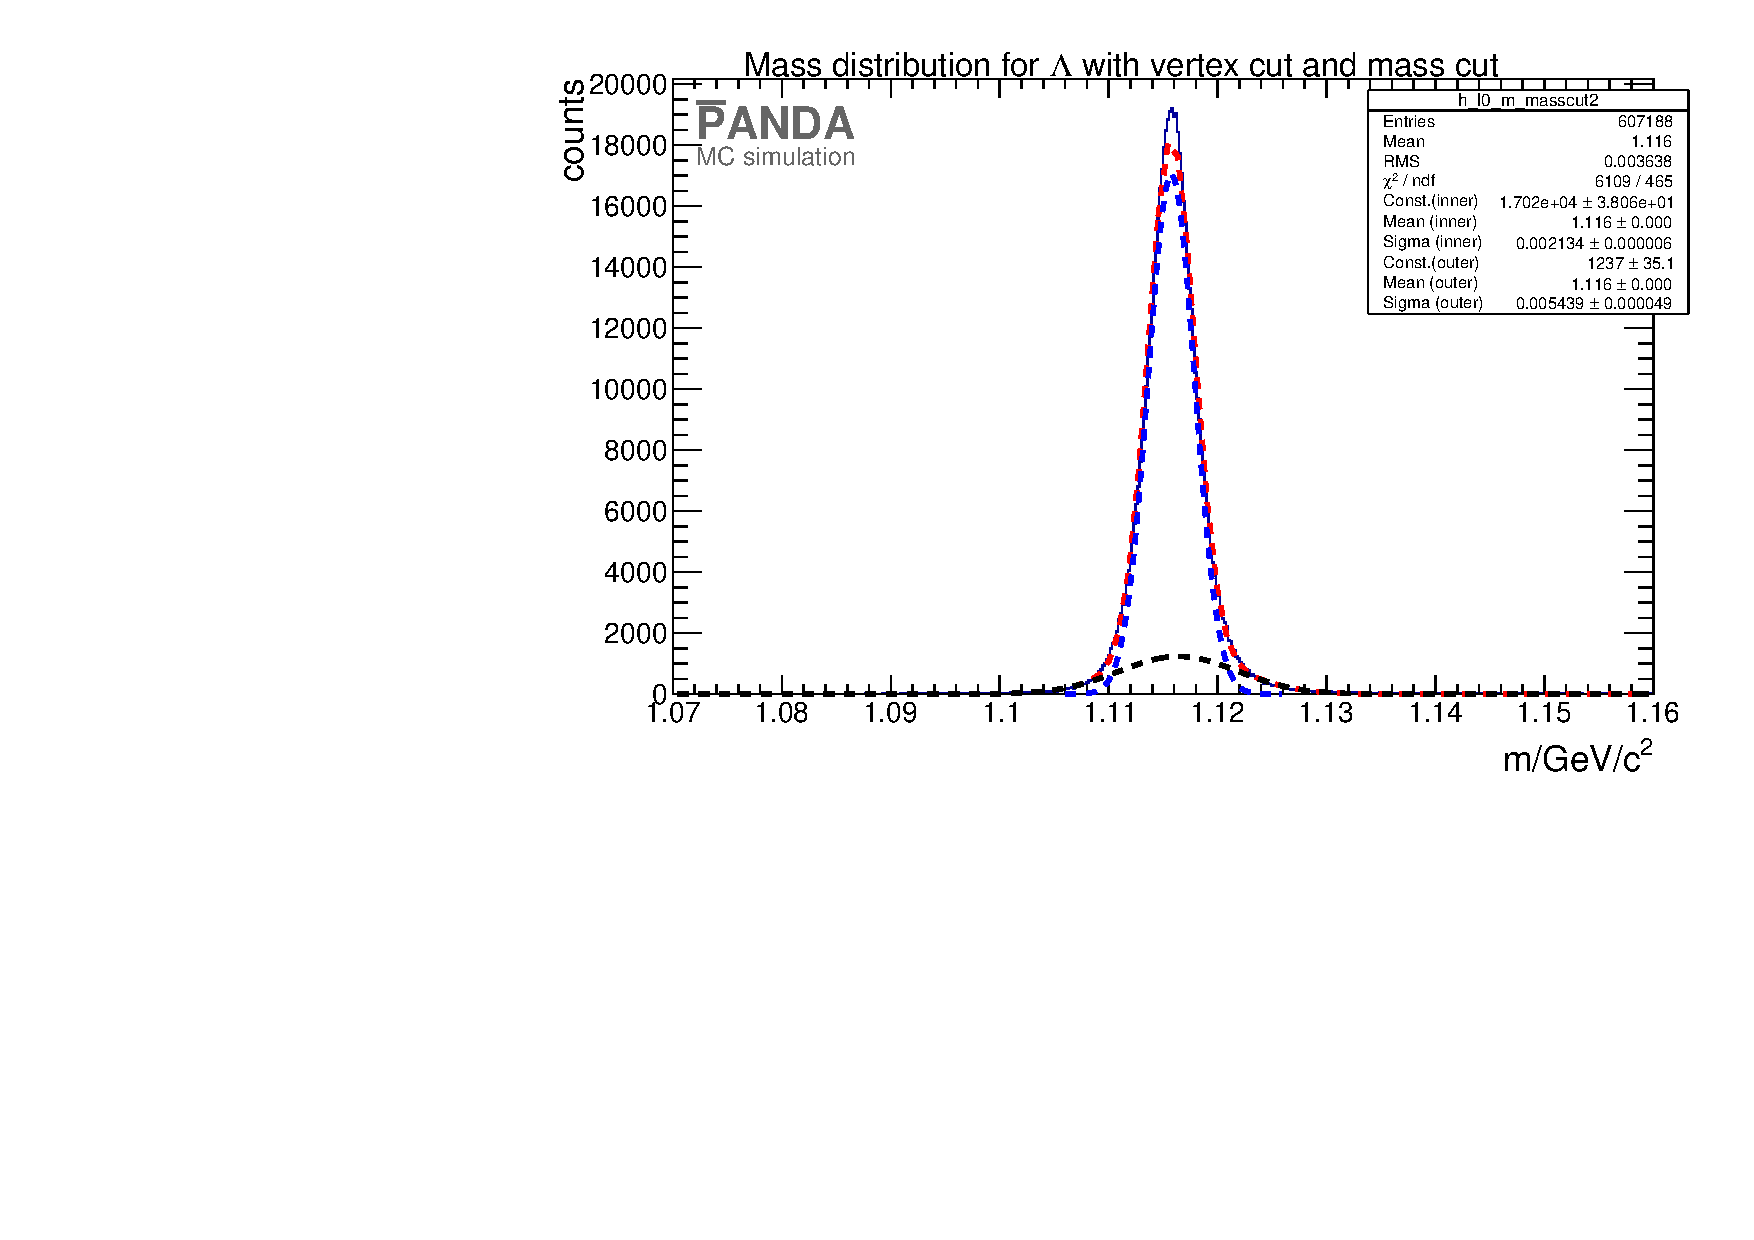
\includegraphics[width=0.8\textwidth]{./plots/lambda0/lambda0_m_masscut2.pdf}
			\caption{\propose Mass distribution -- blue line -- for \lam fitted with a double Gaussian fit shown as red dashed line.}
			\label{fig:lambda0_massfit}
		\end{figure}
		
		The mean value of the inner Gaussian fit is the reconstructed mass.
		The result for \lam is $\mt{m}_{\Lambda^0} = \left(1.116 \pm 3.5\cdot 10^{-5}\right)$ \massunit and for \alam: $\mt{m}_{\bar{\Lambda}^0} = \left(1.116 \pm 1\cdot 10^{-5}\right)$\massunit. 
		The small fit errors could be a result from the wrong covariance matrices. 
		But this has to be checked. 
		Figure \ref{fig:lambda0_pt_vs_pz} shows the transverse momentum versus the longitudinal momentum.
				
		\begin{figure}
			
			\subfigure[]{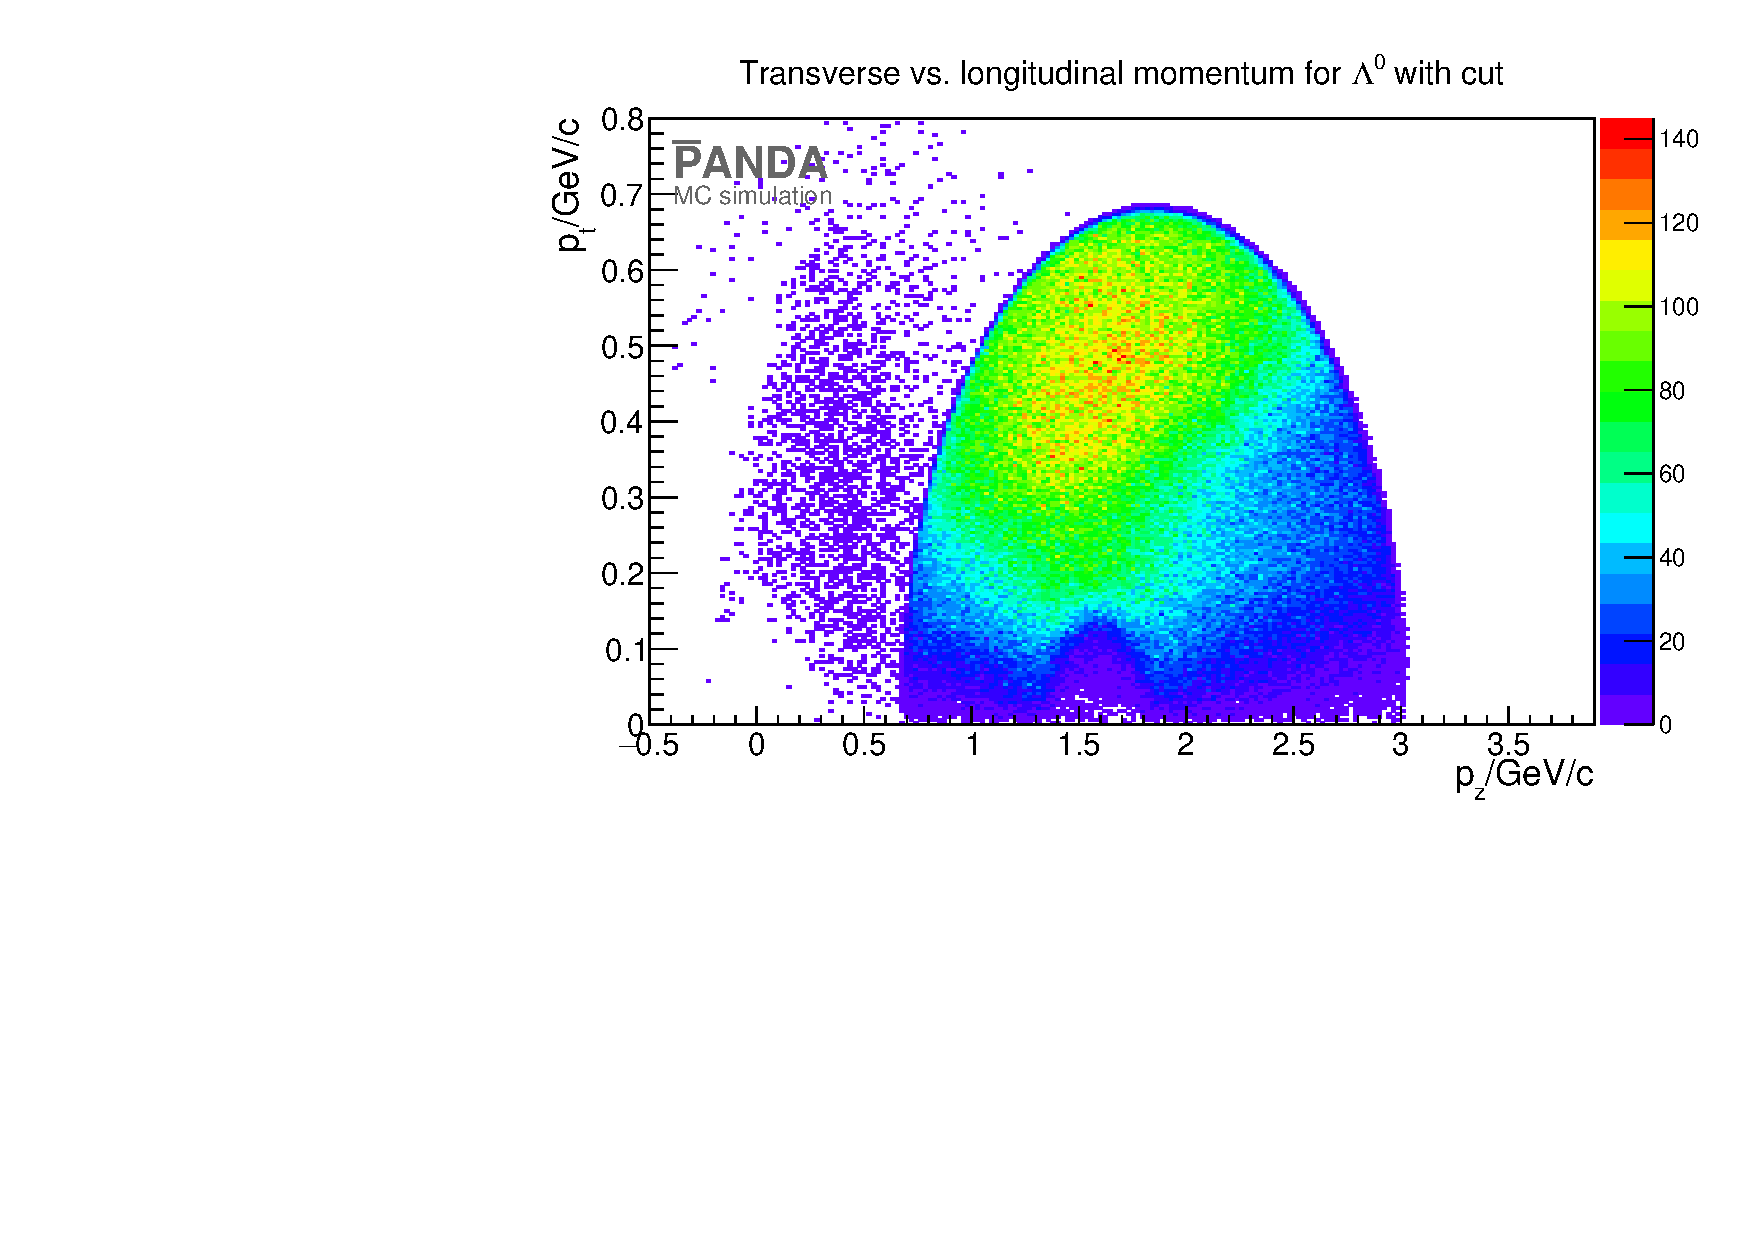
\includegraphics[width=0.49\textwidth]{./plots/lambda0/lambda0_pt_vs_pz_cut.pdf}}
			\subfigure[]{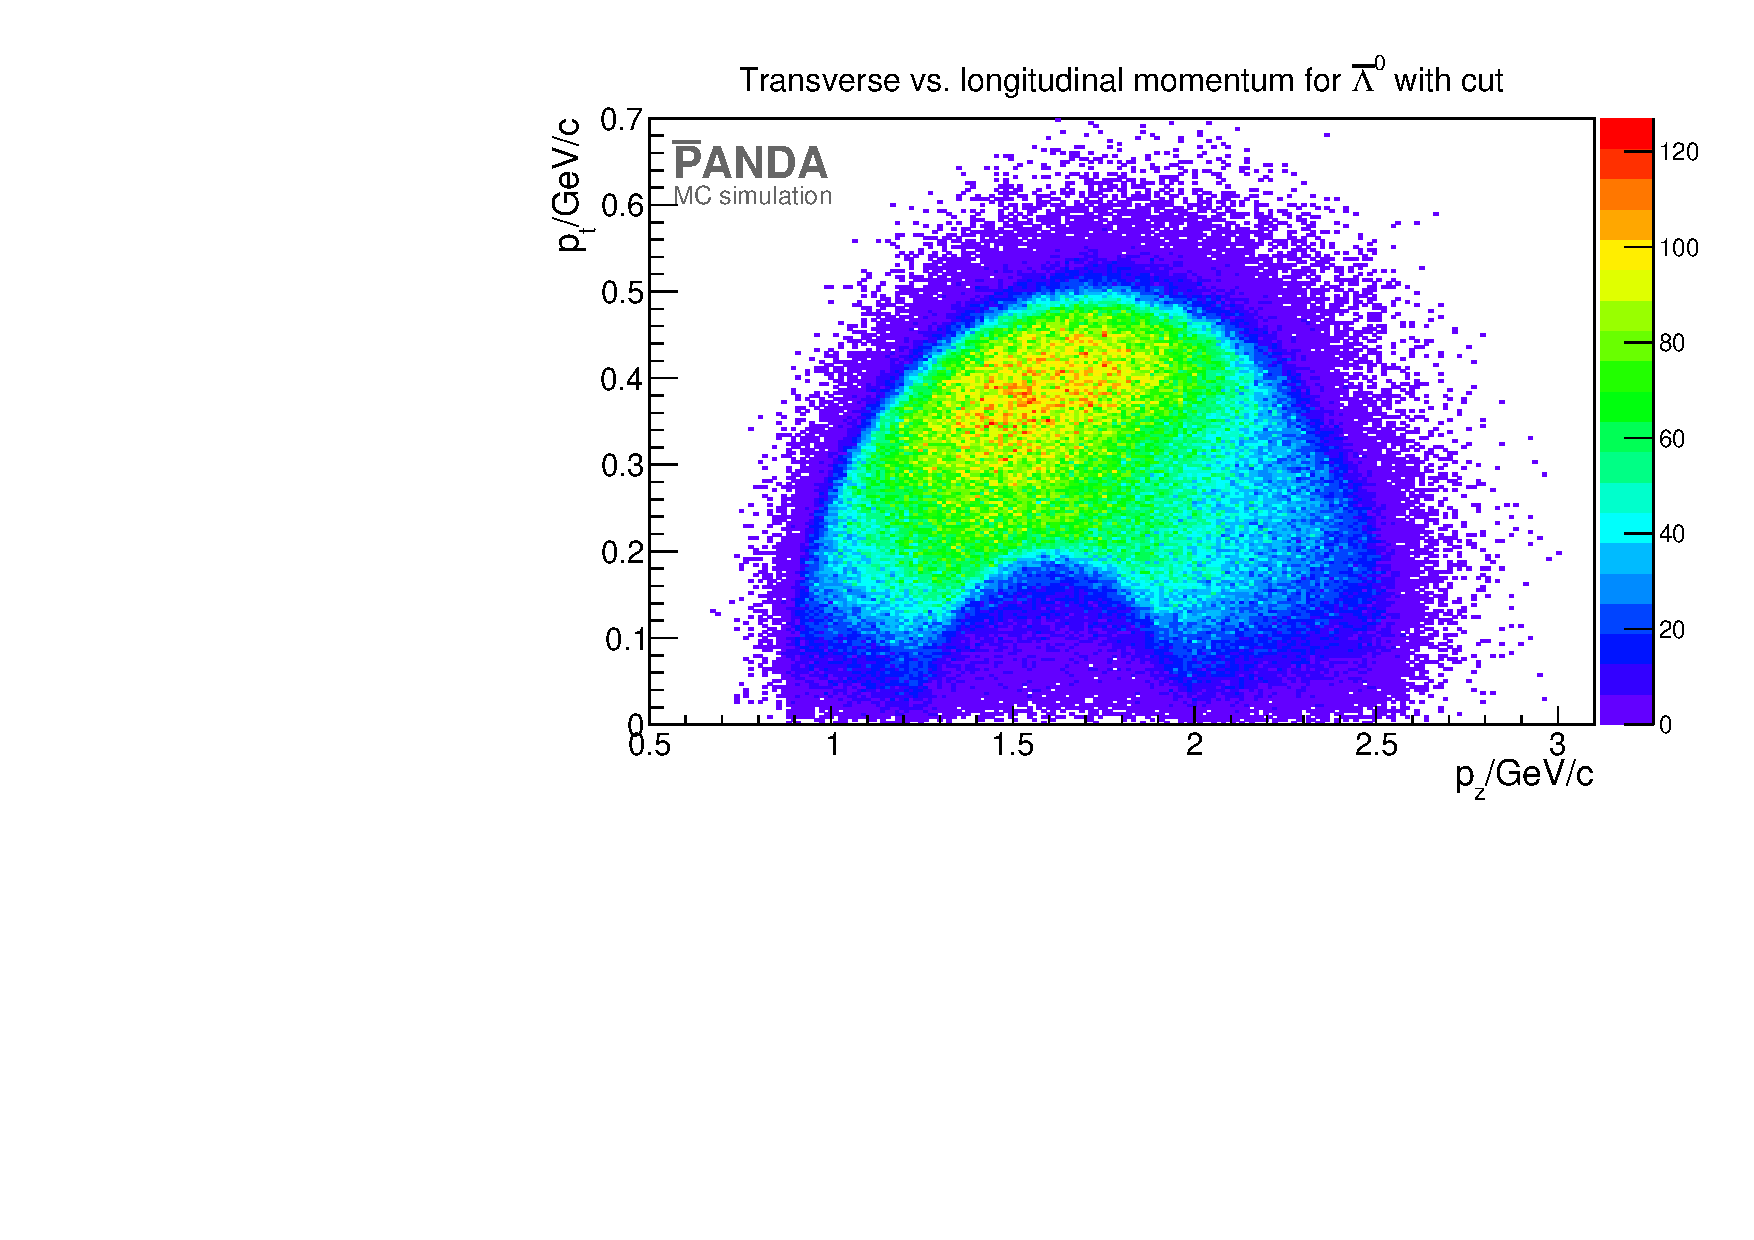
\includegraphics[width=0.49\textwidth]{./plots/antilambda0/antiLambda0_pt_vs_pz_cut.pdf}}
			\caption{\propose The plots shows the transverse against the longitudinal momentum for \lam}
			\label{fig:lambda0_pt_vs_pz}
		
		\end{figure}
		After all cuts the reconstruction efficiency for \lam is $50.33\%$ and for \alam $41.46\%$.
		The difference of the reconstruction efficiency of \lam and \alam is caused by the difference between the decay length of their mother particles.
		\lam is emitted by the \excitedcascade which has a very short decay length while the decay length of \cascade and \anticascade is c$\tau = 4.91 \unit{cm}$ \cite{PDG}.
		In addition the decay length of \lam and \alam is $\textnormal{c}\tau = 7.98 \unit{cm}$.
		If one sum this number up the final state particles of \alam are produced more downstream than the final state particles of \lam.
		This can be also seen in figure \ref{fig:lambda0_antilambda0_decay_vtx}.
		The finale state particles coming from \alam are produced at the edge of the MVD detector so that the reconstruction efficiency get worse.
		
		\begin{figure}
		
			\centering
			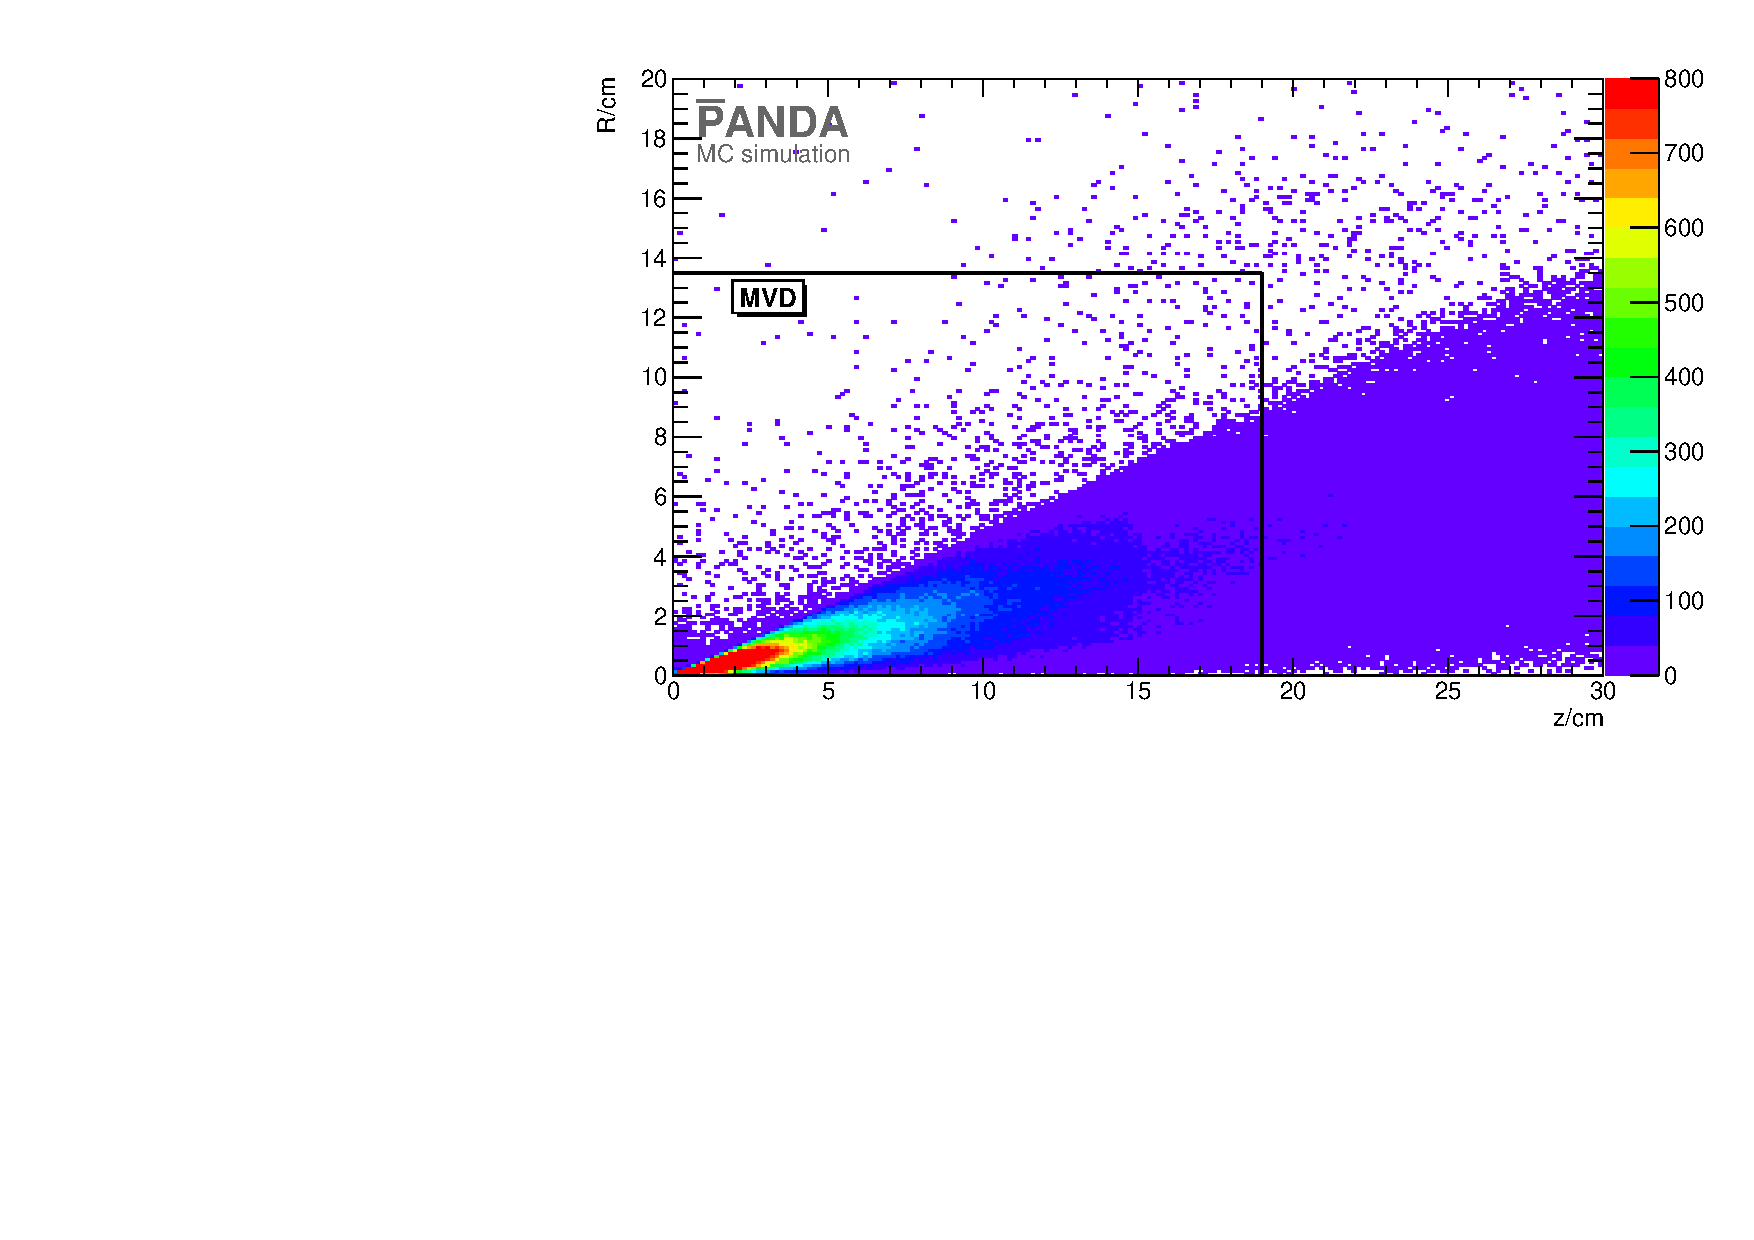
\includegraphics[width=1.\textwidth]{./plots/lambda0/lambda0_decay_vtx.pdf}
			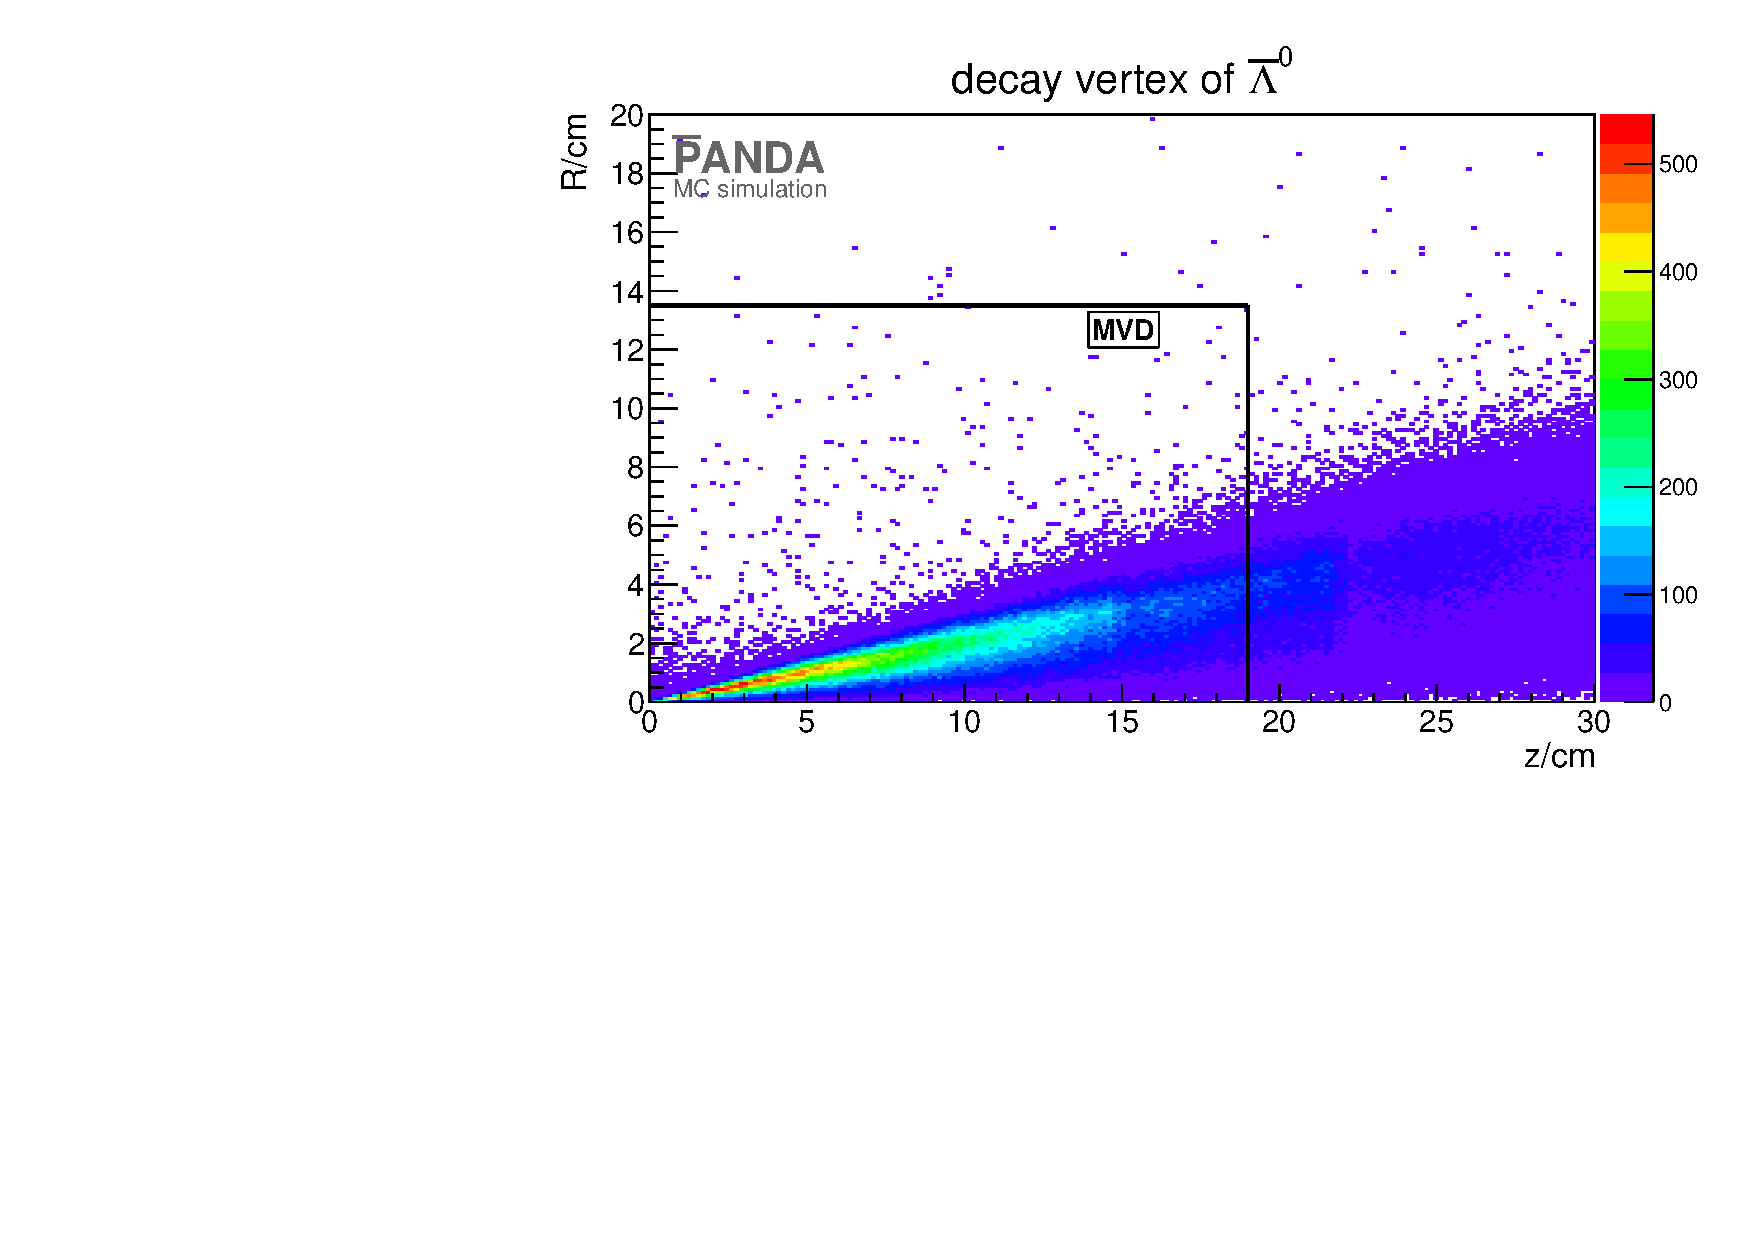
\includegraphics[width=1.\textwidth]{./plots/antilambda0/antiLambda0_decay_vtx.pdf}
			\caption{\propose Upper plot shows the decay vertex of \lam; lower plot shows decay vertex of \alam}
			\label{fig:lambda0_antilambda0_decay_vtx}
		
		\end{figure}
		
		
		
		
	
\section{Reconstruction of $\Xi$ and $\bar{\Xi}$}
	\subsection*{Selection}
		The reconstruction of \cascade and \anticascade fellow a similar scheme like for \lam and \alam.
		For \anticascade are \alam and \piplusone recombined and for \cascade in the c.c. channel \lam and \piminusone.
		Now it is distinguished between the to \piplus (\piminus) particle and use only those particles which have not already been combined.
		After combining the daughter particles it is performed a mass window cut with width of $0.3$\massunit 
		around the \cascade mass $m_{\Xi} = 1.32171$ \massunit \cite{PDG}.
		 
		The fitting scheme is the same as for \lam and \alam and is shown in figure \ref{fig:anticascade_scheme} 
		After the mass window cut the daughter particles are fitted to a common vertex with the PndKinVtxFitter.
		And again these information is used to perform the mass constraint fitter. 
		
		\begin{figure}
			\centering
				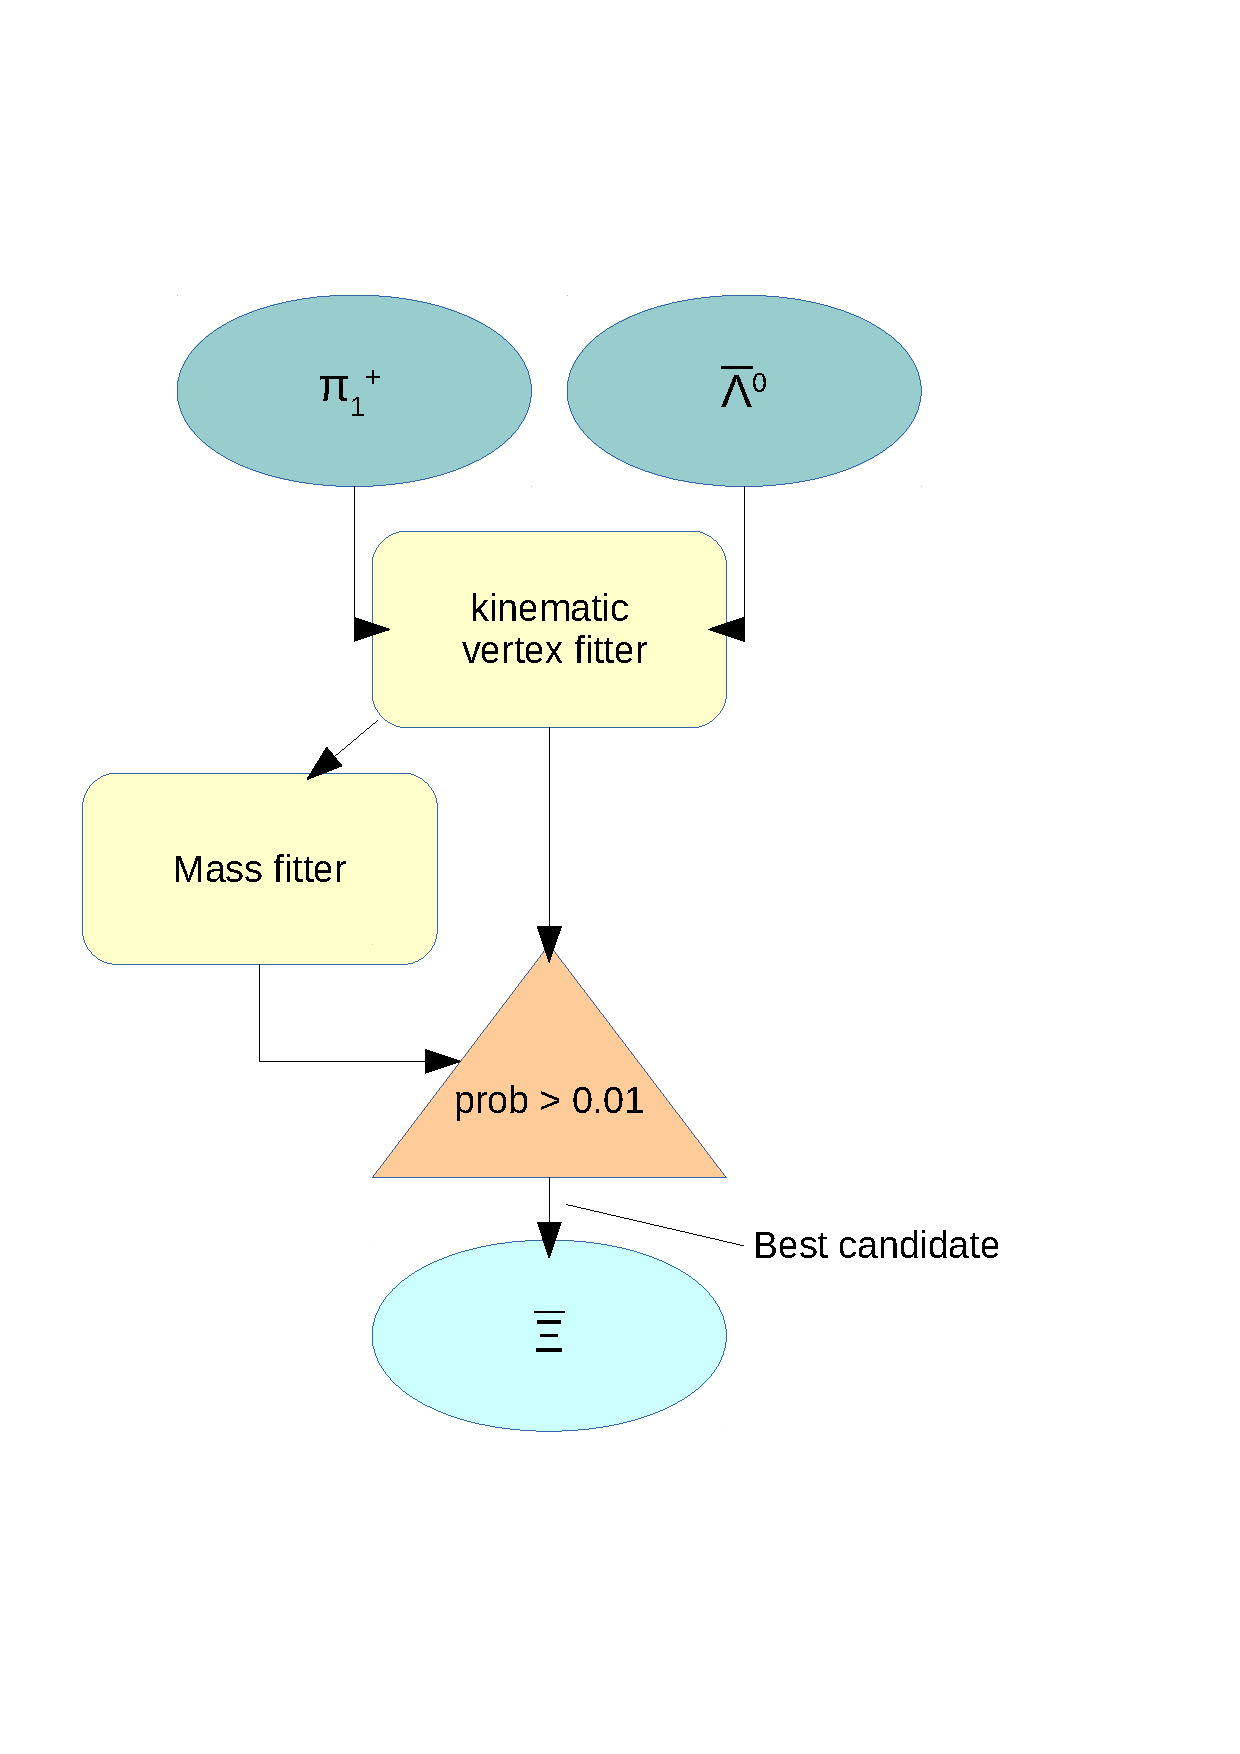
\includegraphics[width=0.50\textwidth]{./plots/combineAntiCascade.pdf}
			\caption{\propose Scheme for \anticascade reconstruction}
			\label{fig:anticascade_scheme}
		\end{figure}
		
		Only those particles are selected which have a \chisq probability of more than $1\,\%$ in both fitter. 
		Figure \ref{fig:XiPlus_prob} shows exemplarily the cut on the vertex fit probability.
		
		\begin{figure}
			\centering
				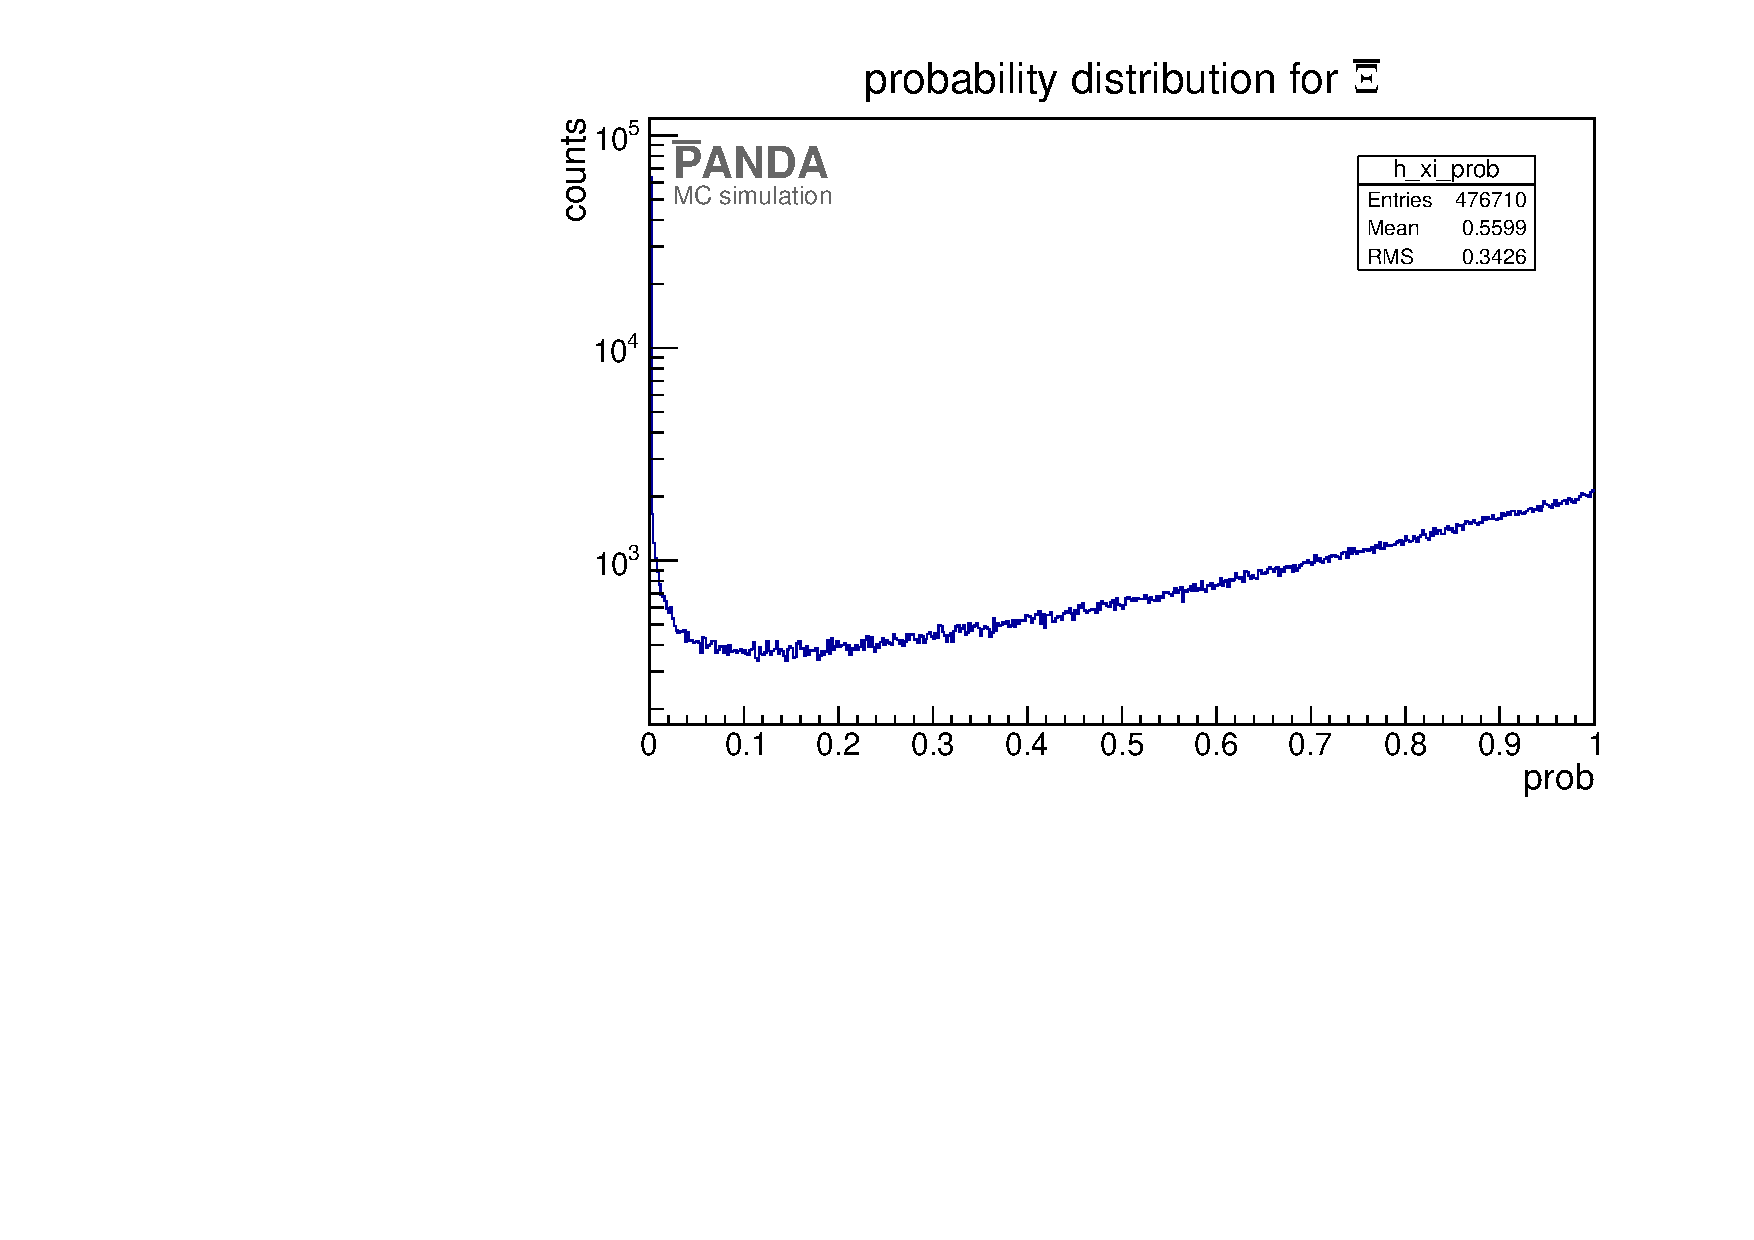
\includegraphics[width=0.50\textwidth]{./plots/Xi/XiPlus_prob.pdf}
			\caption{\propose \chisq probability for \anticascade reconstruction}
			\label{fig:XiPlus_prob}
		\end{figure}
			
		If there is more than one candidate left after all cuts the best candidate is chosen.
		
		
	\subsection*{Results}
		The vertex resolution after all cuts is shown in table \ref{tab:XiPlus_vtxres}. 
		
		\begin{table}
			\centering
			\caption{\propose Vertex resolution for \anticascade and \cascade (c.c. channel)}
			\label{tab:XiPlus_vtxres}
			\begin{tabular}{ccc}
				\hline
				position & \anticascade & \cascade(from c.c.) \\\hline
				\hline
				x/cm & $0.052$ & $0.056$\\
				y/cm & $0.052$ & $0.052$\\
				z/cm & $0.192$ & $0.2$\\
				\hline
				    
			\end{tabular}
		\end{table}
		
		It is determined by calculating the full width at half maximum (FWHM) of the distribution.
		The advantage of using this method to calculated the vertex resolution is that the FWHM is independent of distribution shape.
		Figure \ref{fig:xi_vtxres_x} and Figure \ref{fig:xi_vtxres_yz} show the vertex resolution. 
		
		\begin{figure}
			\centering
			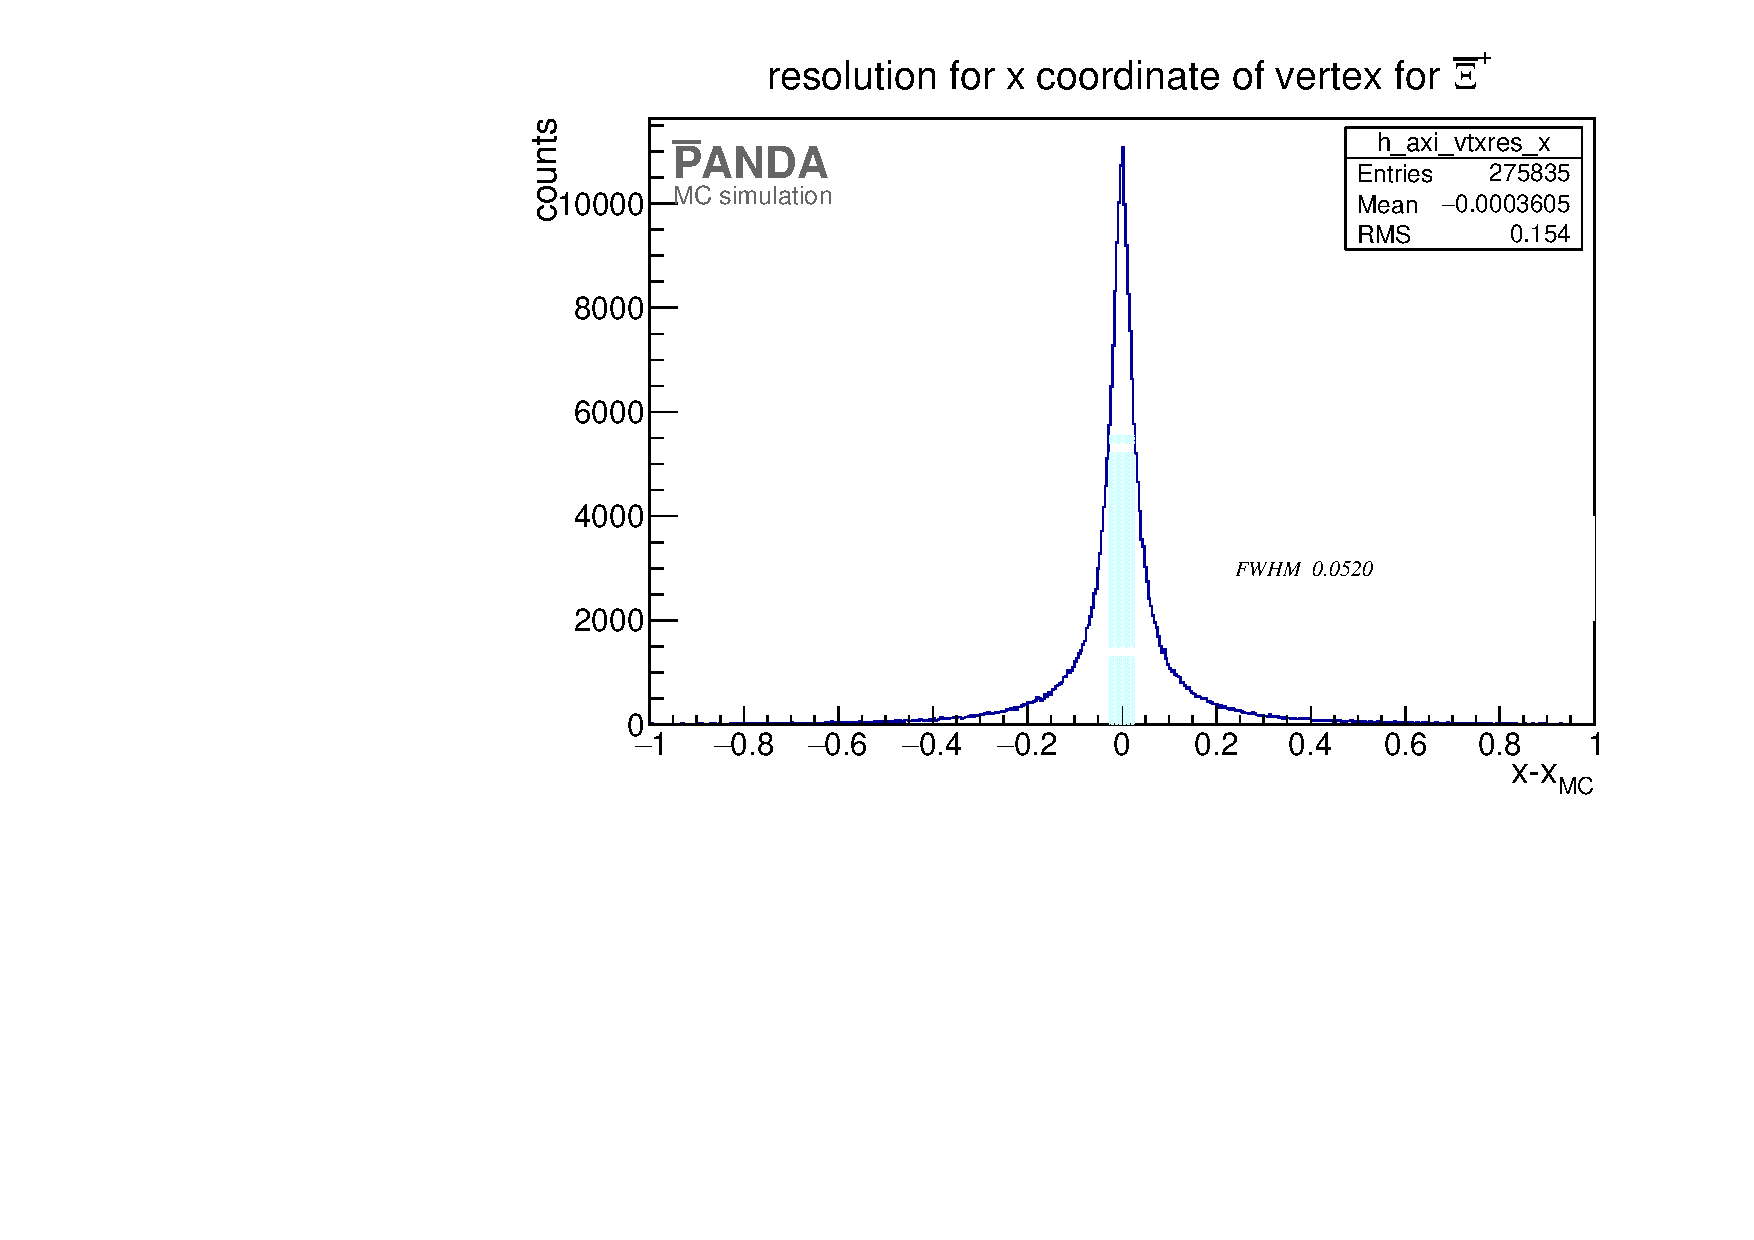
\includegraphics[width=0.8\textwidth]{./plots/Xi/XiPlus_vtxres_x.pdf}
			\caption{\propose Vertex resolution of x position for \anticascade}
			\label{fig:xi_vtxres_x}
			
		\end{figure}
		
		\begin{figure}
			\subfigure[Vertex resolution for y coordinate]{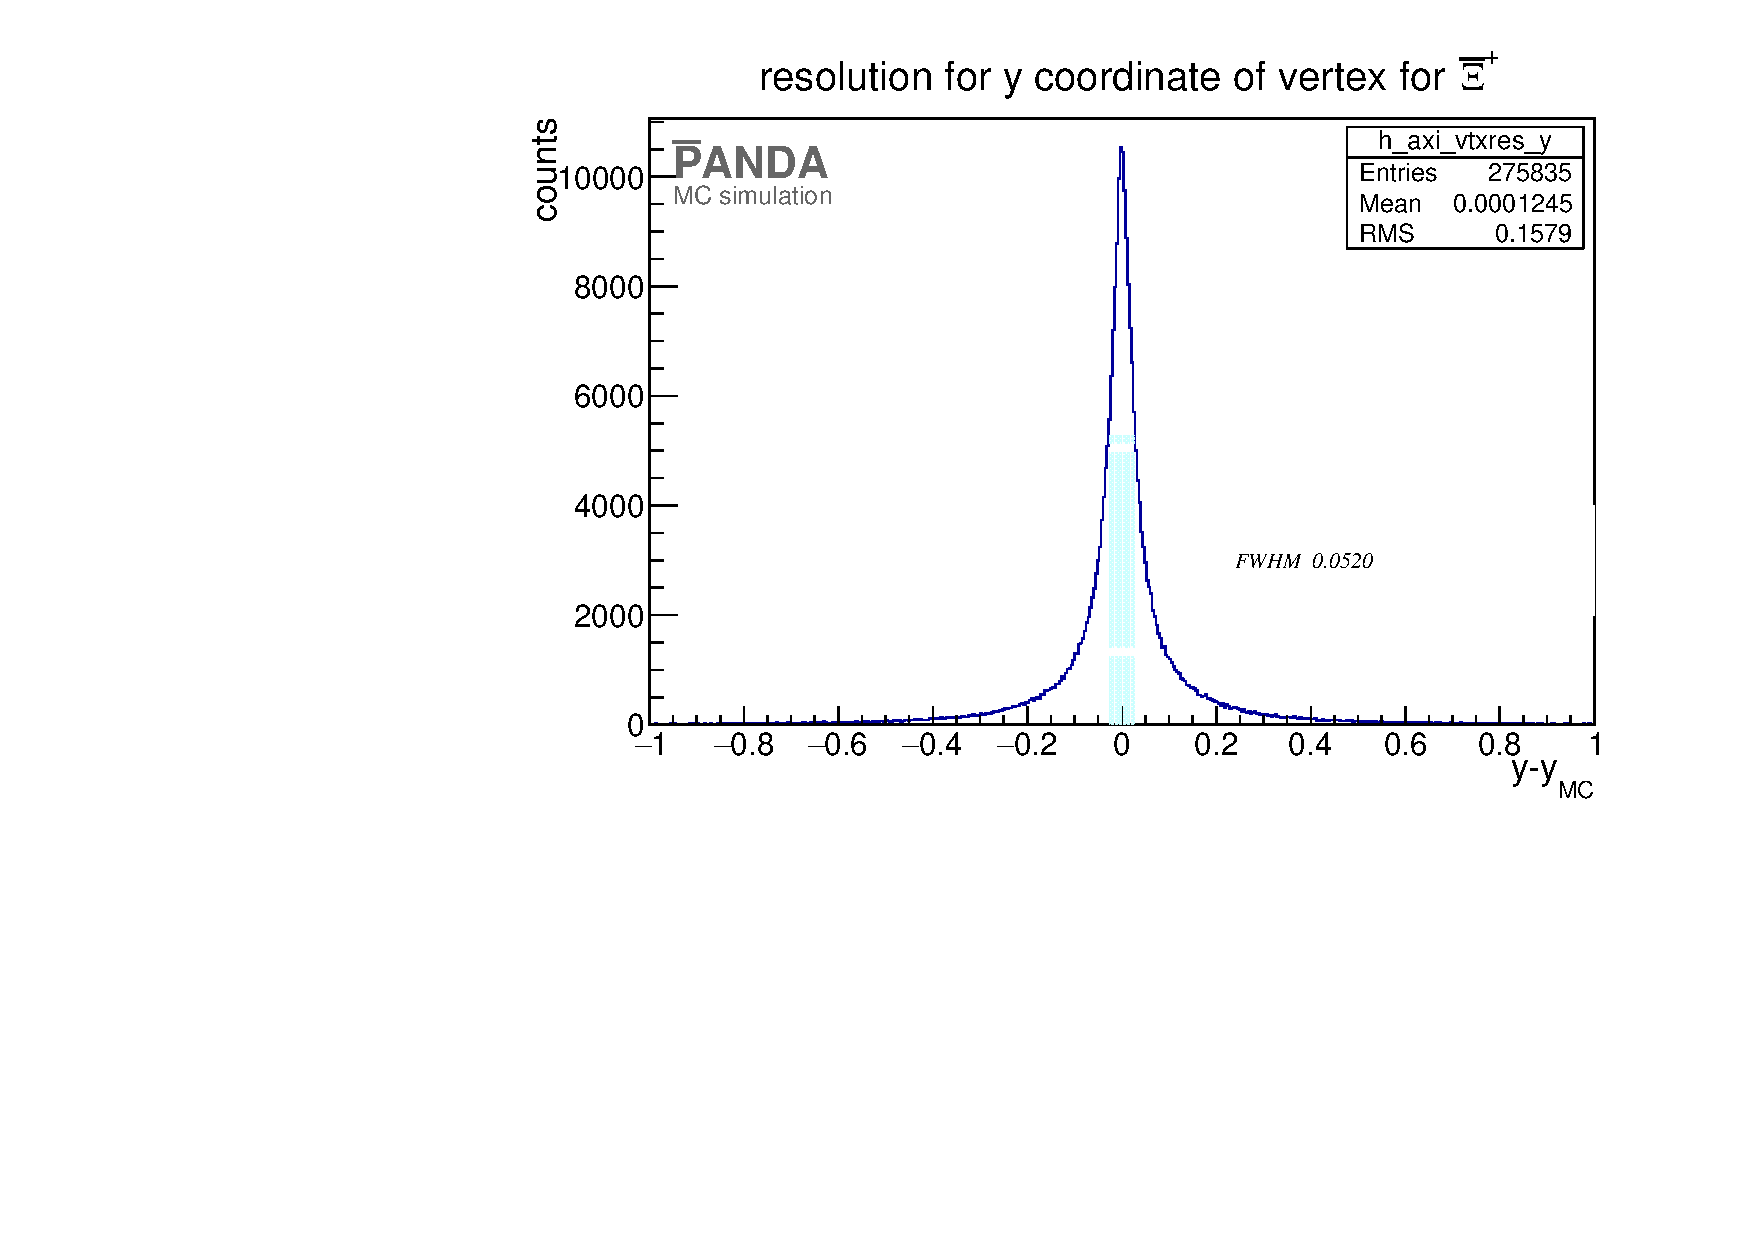
\includegraphics[width=0.49\textwidth]{./plots/Xi/XiPlus_vtxres_y.pdf}}
			\subfigure[Vertex resolution for z coordinate]{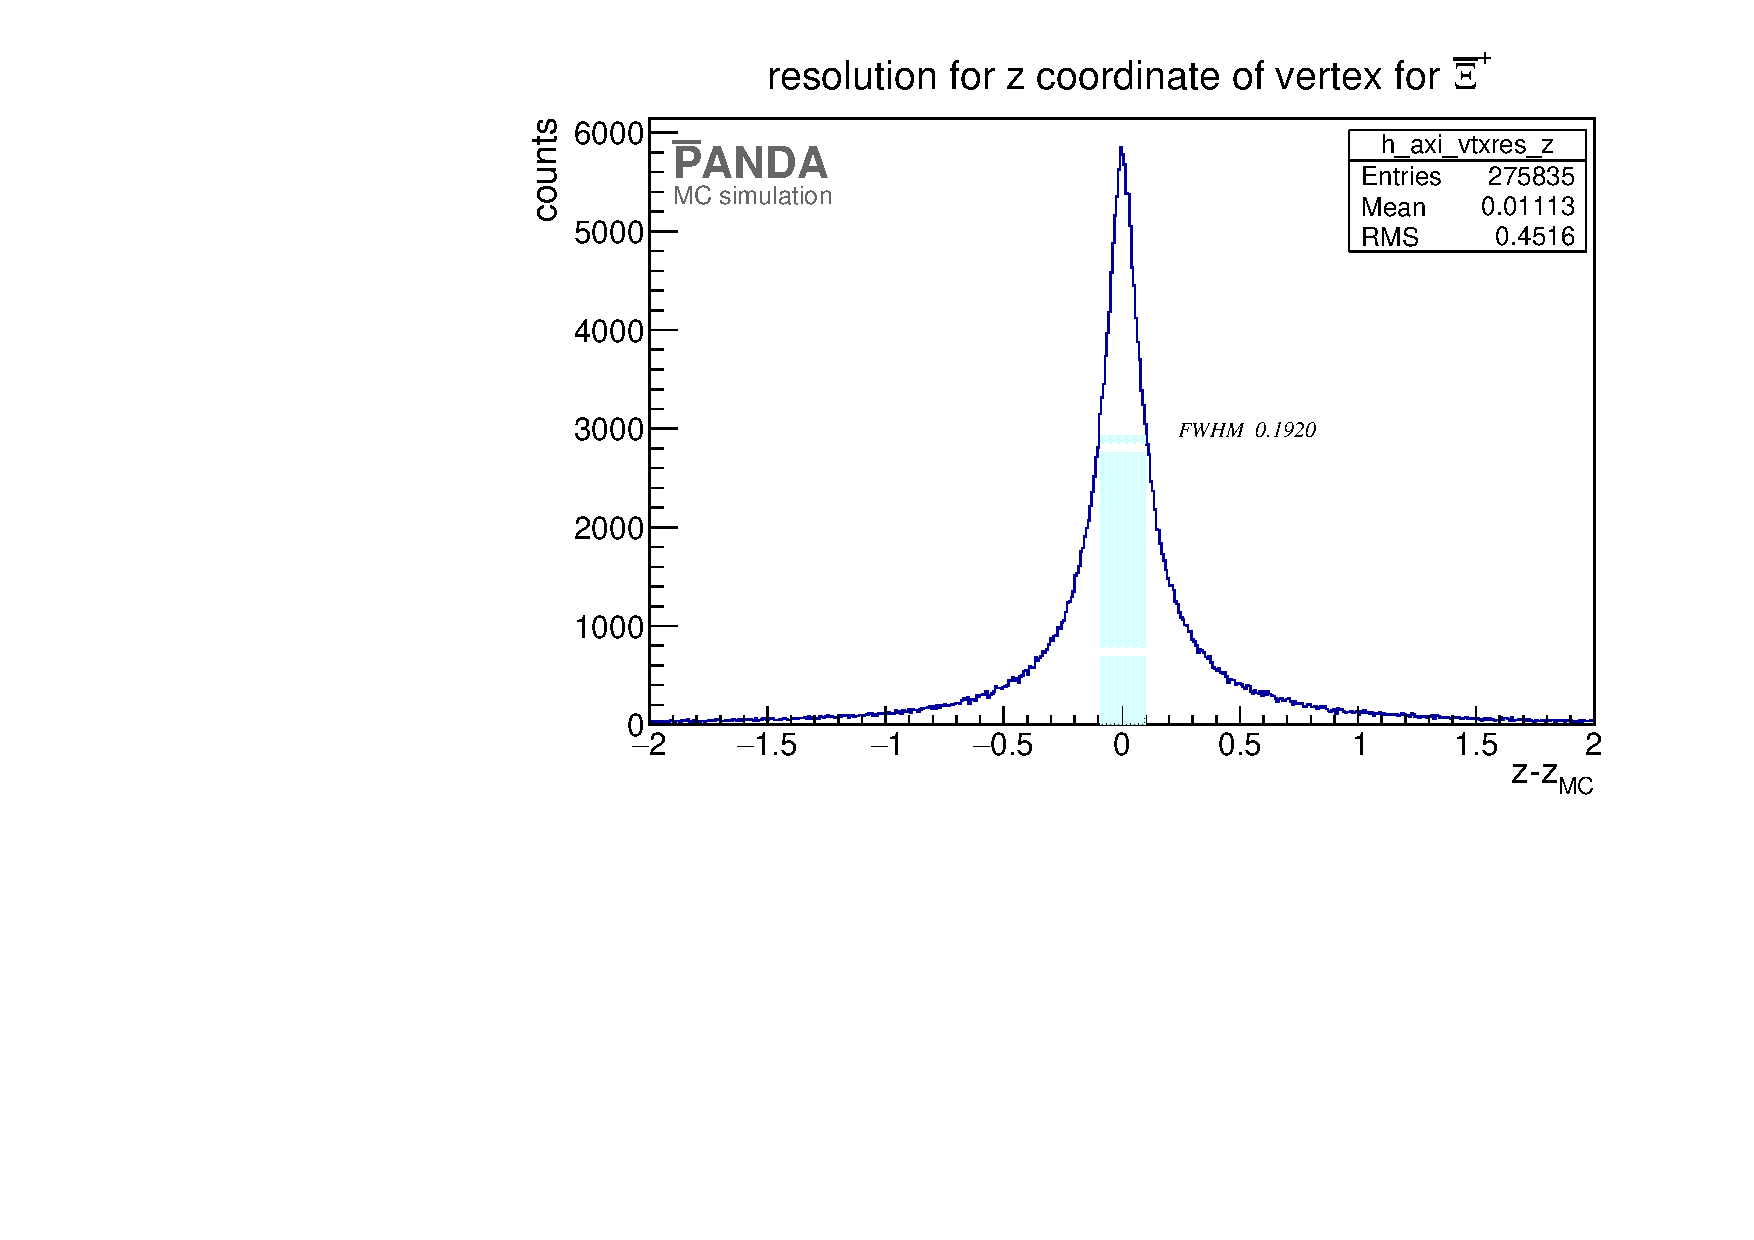
\includegraphics[width=0.49\textwidth]{./plots/Xi/XiPlus_vtxres_z.pdf}}
			\caption{\propose left plot: Vertex resolution of y position for \anticascade; right plot: Vertex resolution of z position for \anticascade.}
			\label{fig:xi_vtxres_yz}
			
		\end{figure}
	
		The mass distribution for the different cuts is shown in figure \ref{fig:XiPlus_massdiffcuts} and figure \ref{fig:XiMinus_massdiffcuts}. 
		The vertex fitter cut reduces the number of events most and the width of the mass distribution gets smaller.
		
		\begin{figure}
			\centering
				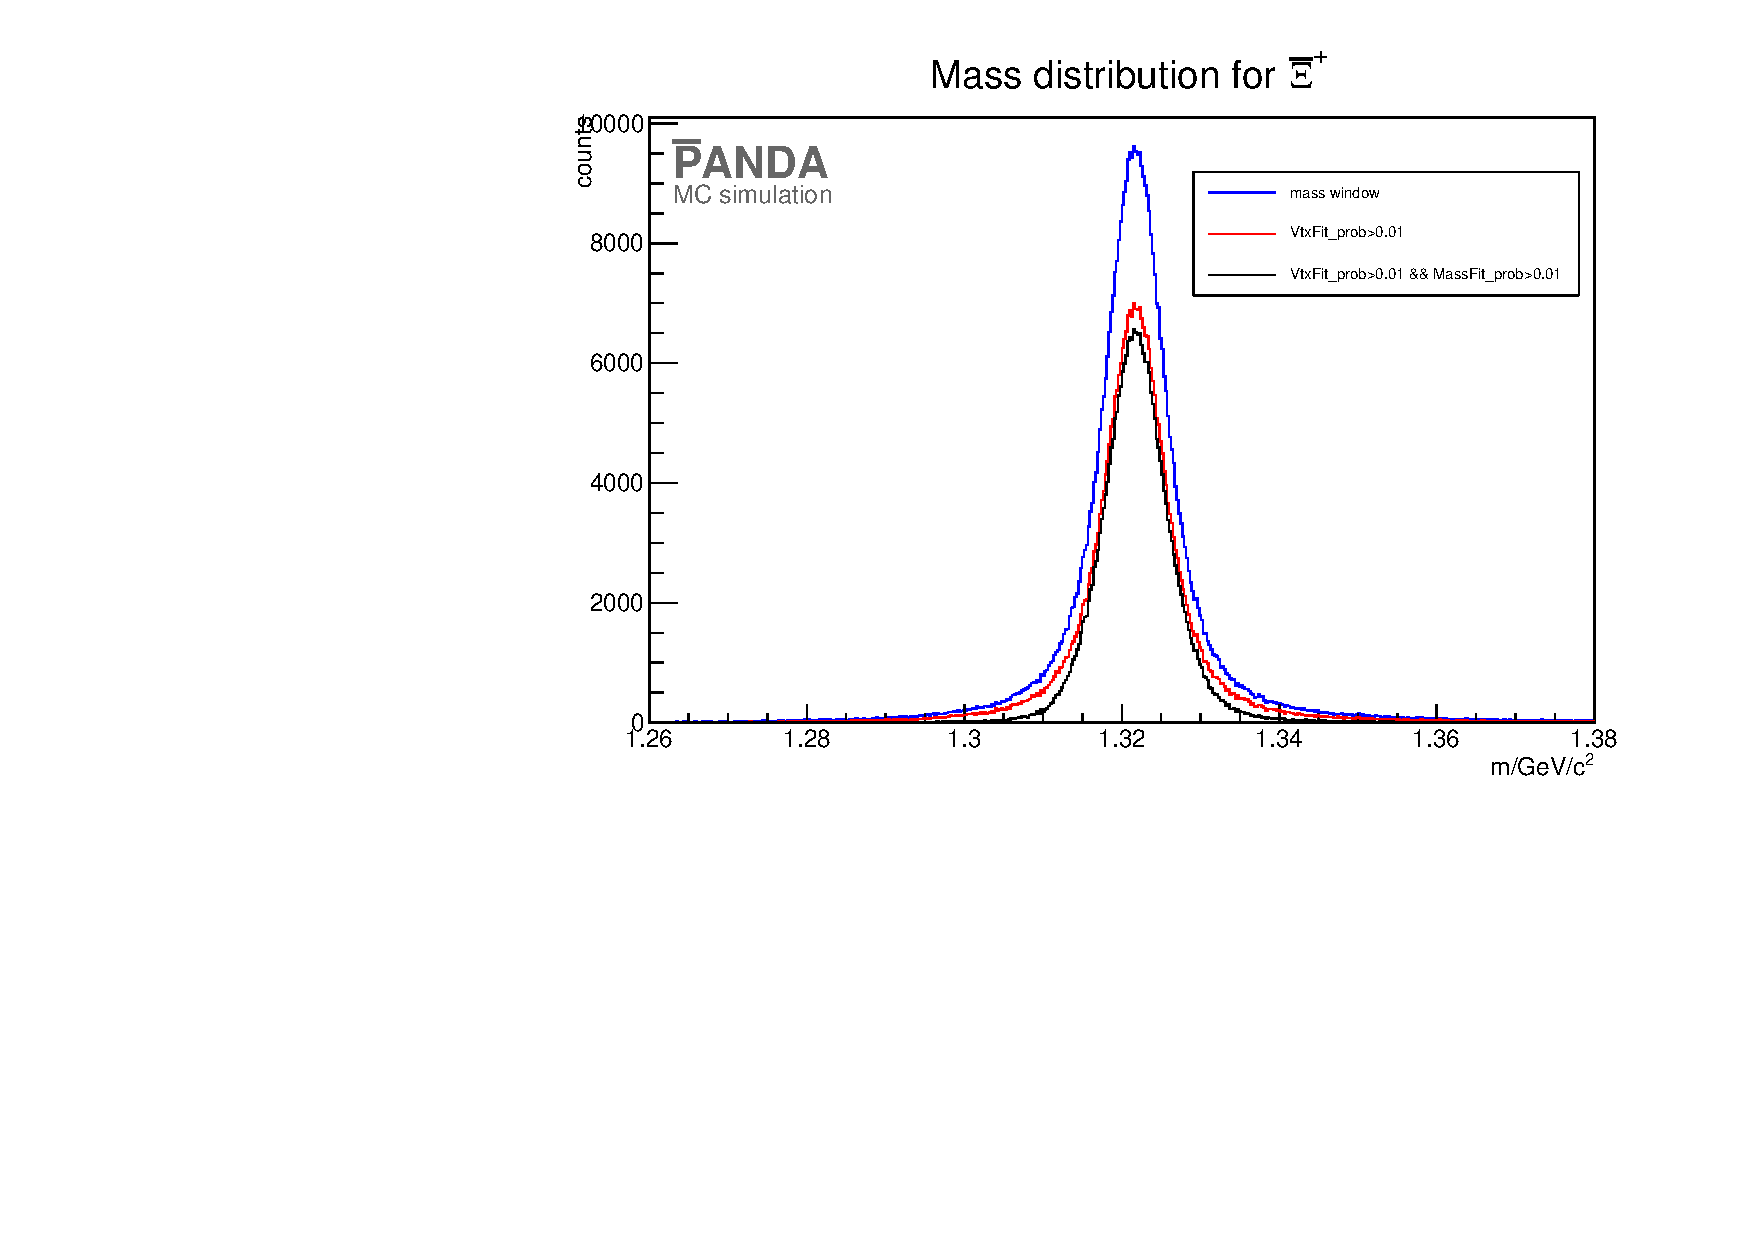
\includegraphics[width=1.1\textwidth]{./plots/Xi/XiPlus_m_diffcuts.pdf}
			\caption{\propose Mass distribution of \anticascade for different cuts}
			\label{fig:XiPlus_massdiffcuts}
			
				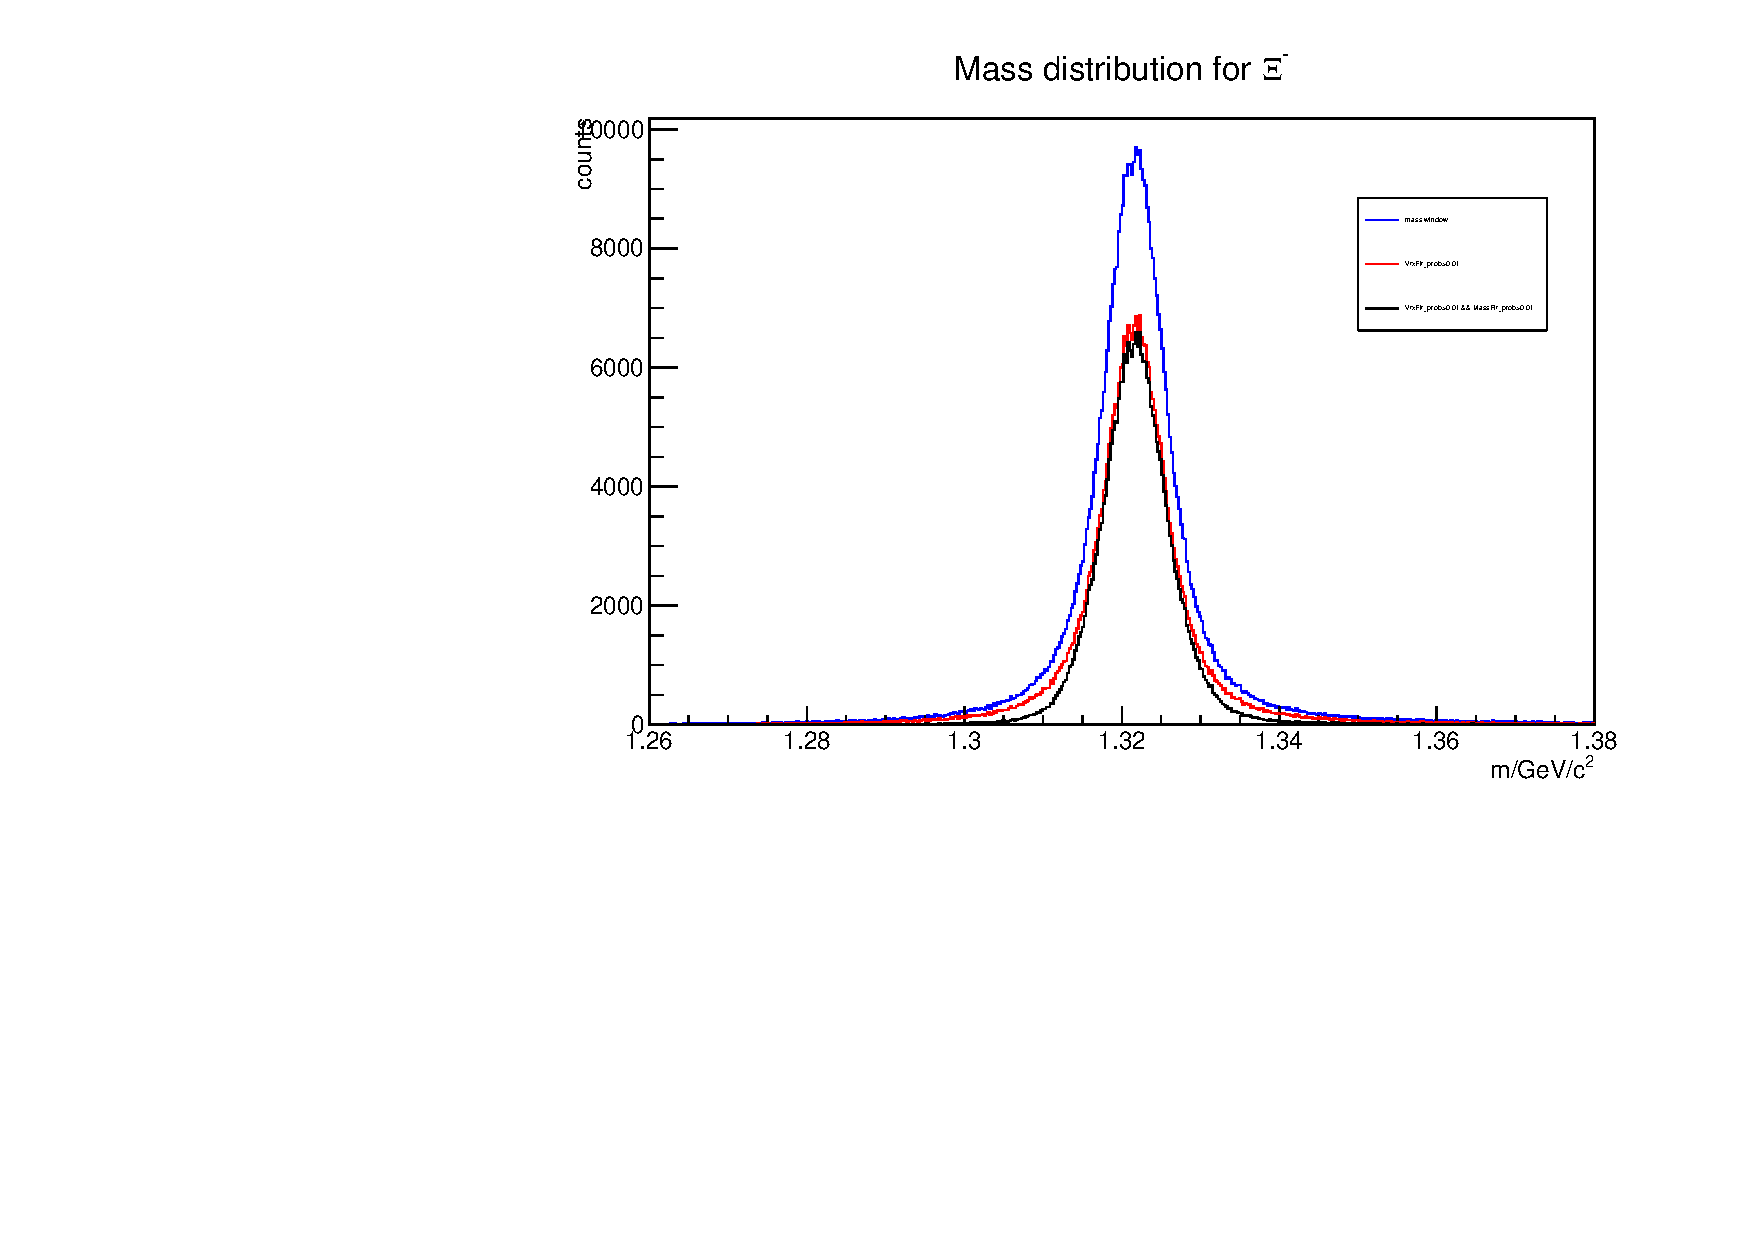
\includegraphics[width=1.1\textwidth]{./plots/Xi/XiMinus_m_diffcuts.pdf}
			\caption{\propose Mass distribution of \cascade for different cuts}
			\label{fig:XiMinus_massdiffcuts}
		\end{figure}
		
		After using all cuts on the mass distribution the reconstructed mass of \cascade and \anticascade can be determined by a double Gaussian fit.
		This is exemplarily shown for the \cascade in figure \ref{fig:XiPlus_massfit}.
		
		\begin{figure}
			\centering
				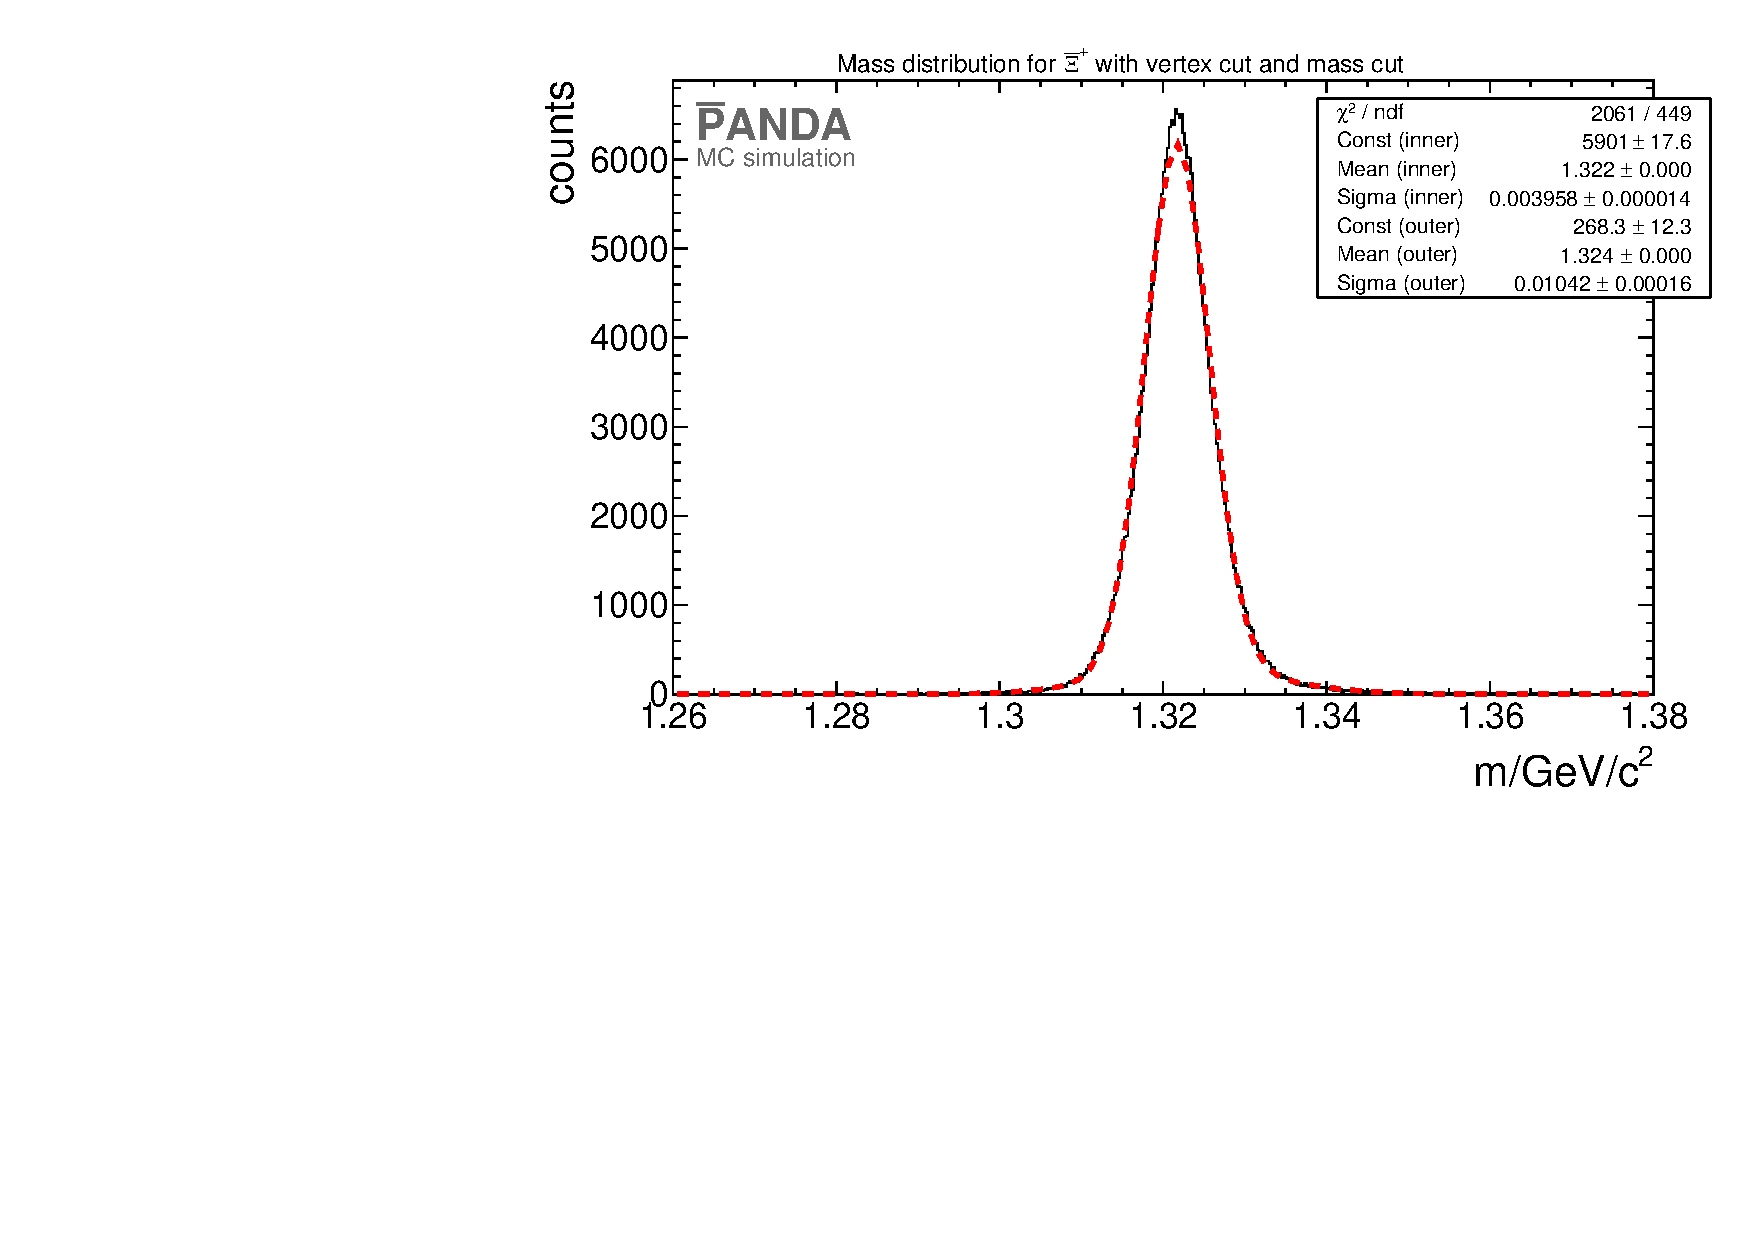
\includegraphics[width=0.8\textwidth]{./plots/Xi/XiPlus_m_masscut.pdf}
			\caption{\propose Mass fit with a double Gaussian fit}
			\label{fig:XiPlus_massfit}
		\end{figure}
		The result of the mass fit is for \anticascade $\mt{m} = \left( 1.3721716 \pm 9.2\cdot 10^{-5}\right)$ \massunit 
		and for \cascade $\mt{m} = \left( 1\pm 1\cdot 10^{-5}\right)$ \massunit.
		The two dimensional momentum distribution for \anticascade and \cascade is shown in figure \ref{fig:XiPlus_pt_vs_pz} 
		
		\begin{figure}
			\subfigure[\anticascade]{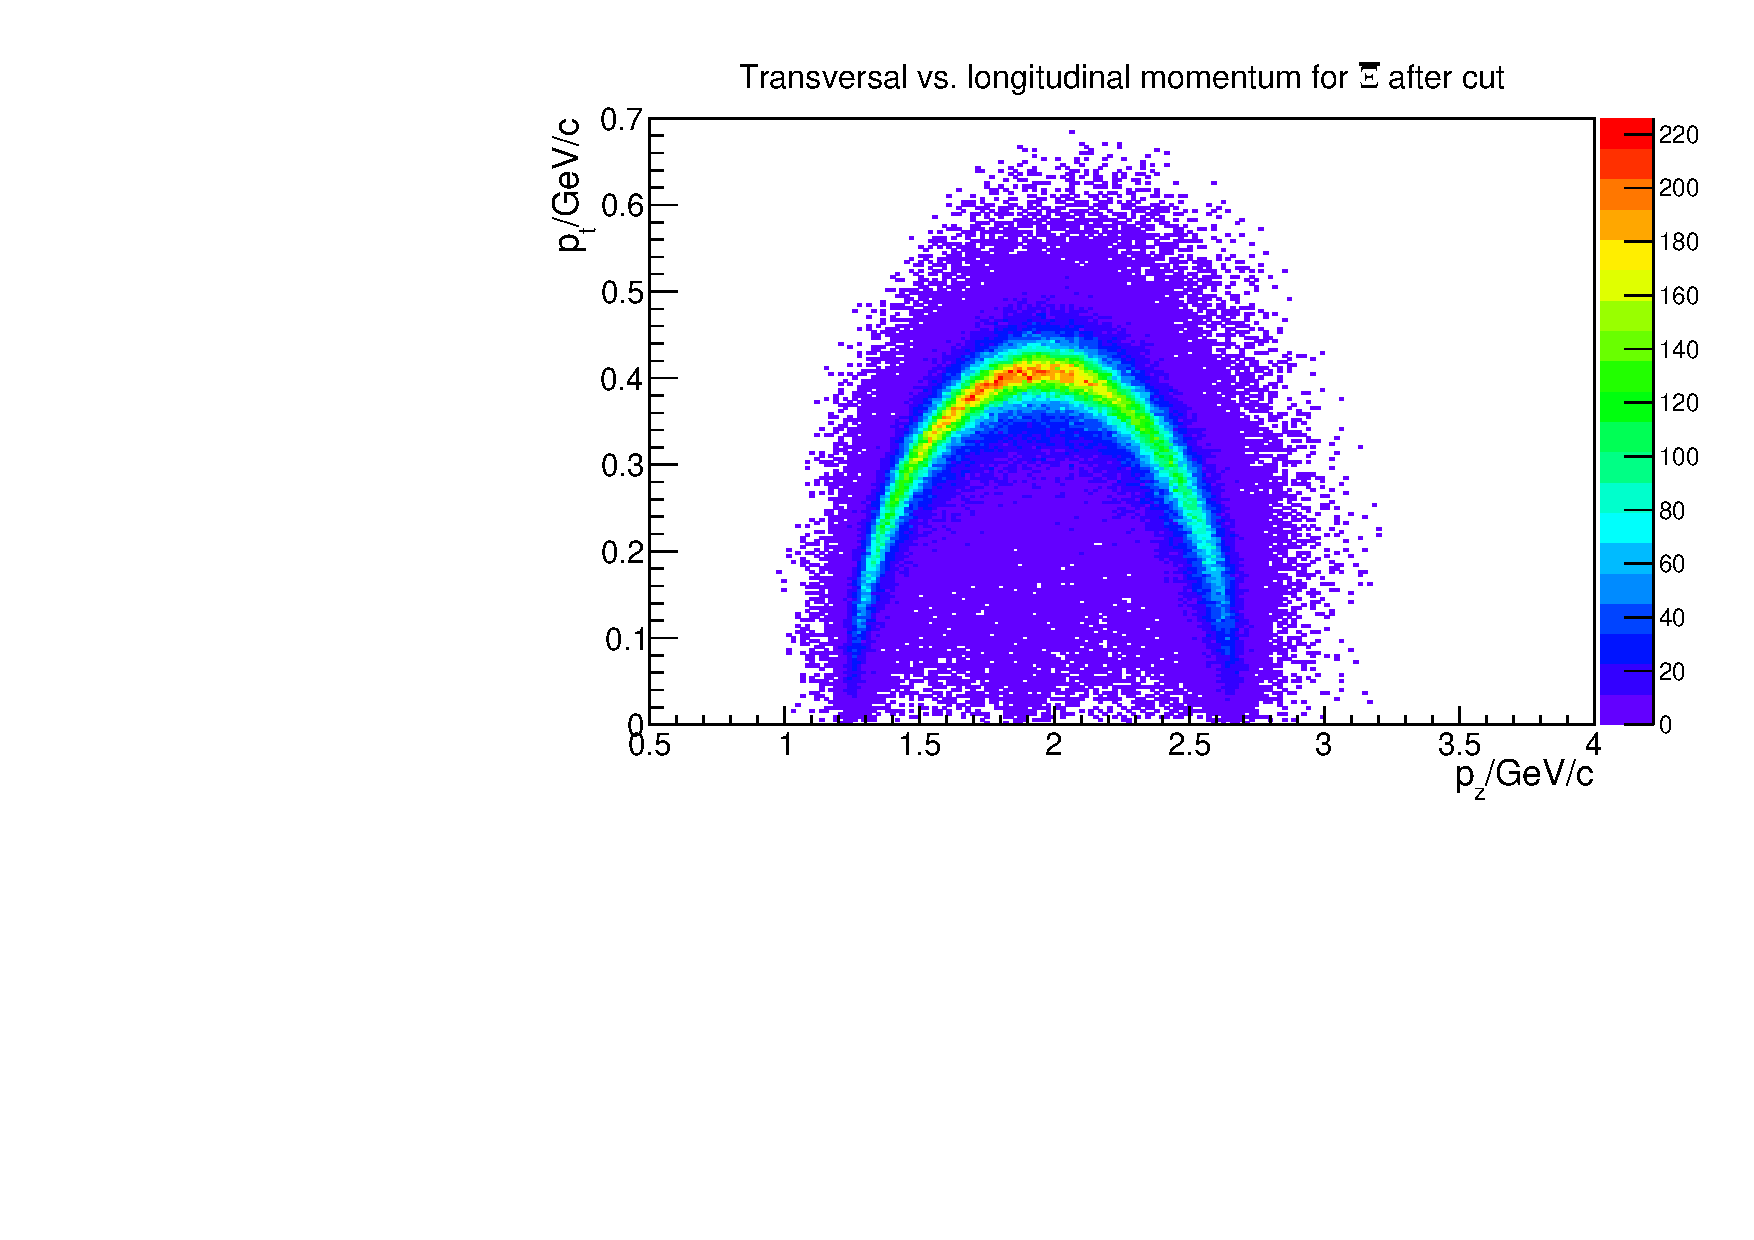
\includegraphics[width=0.49\textwidth]{./plots/Xi/XiPlus_pt_vs_pz_cut.pdf}}
			\subfigure[\cascade]{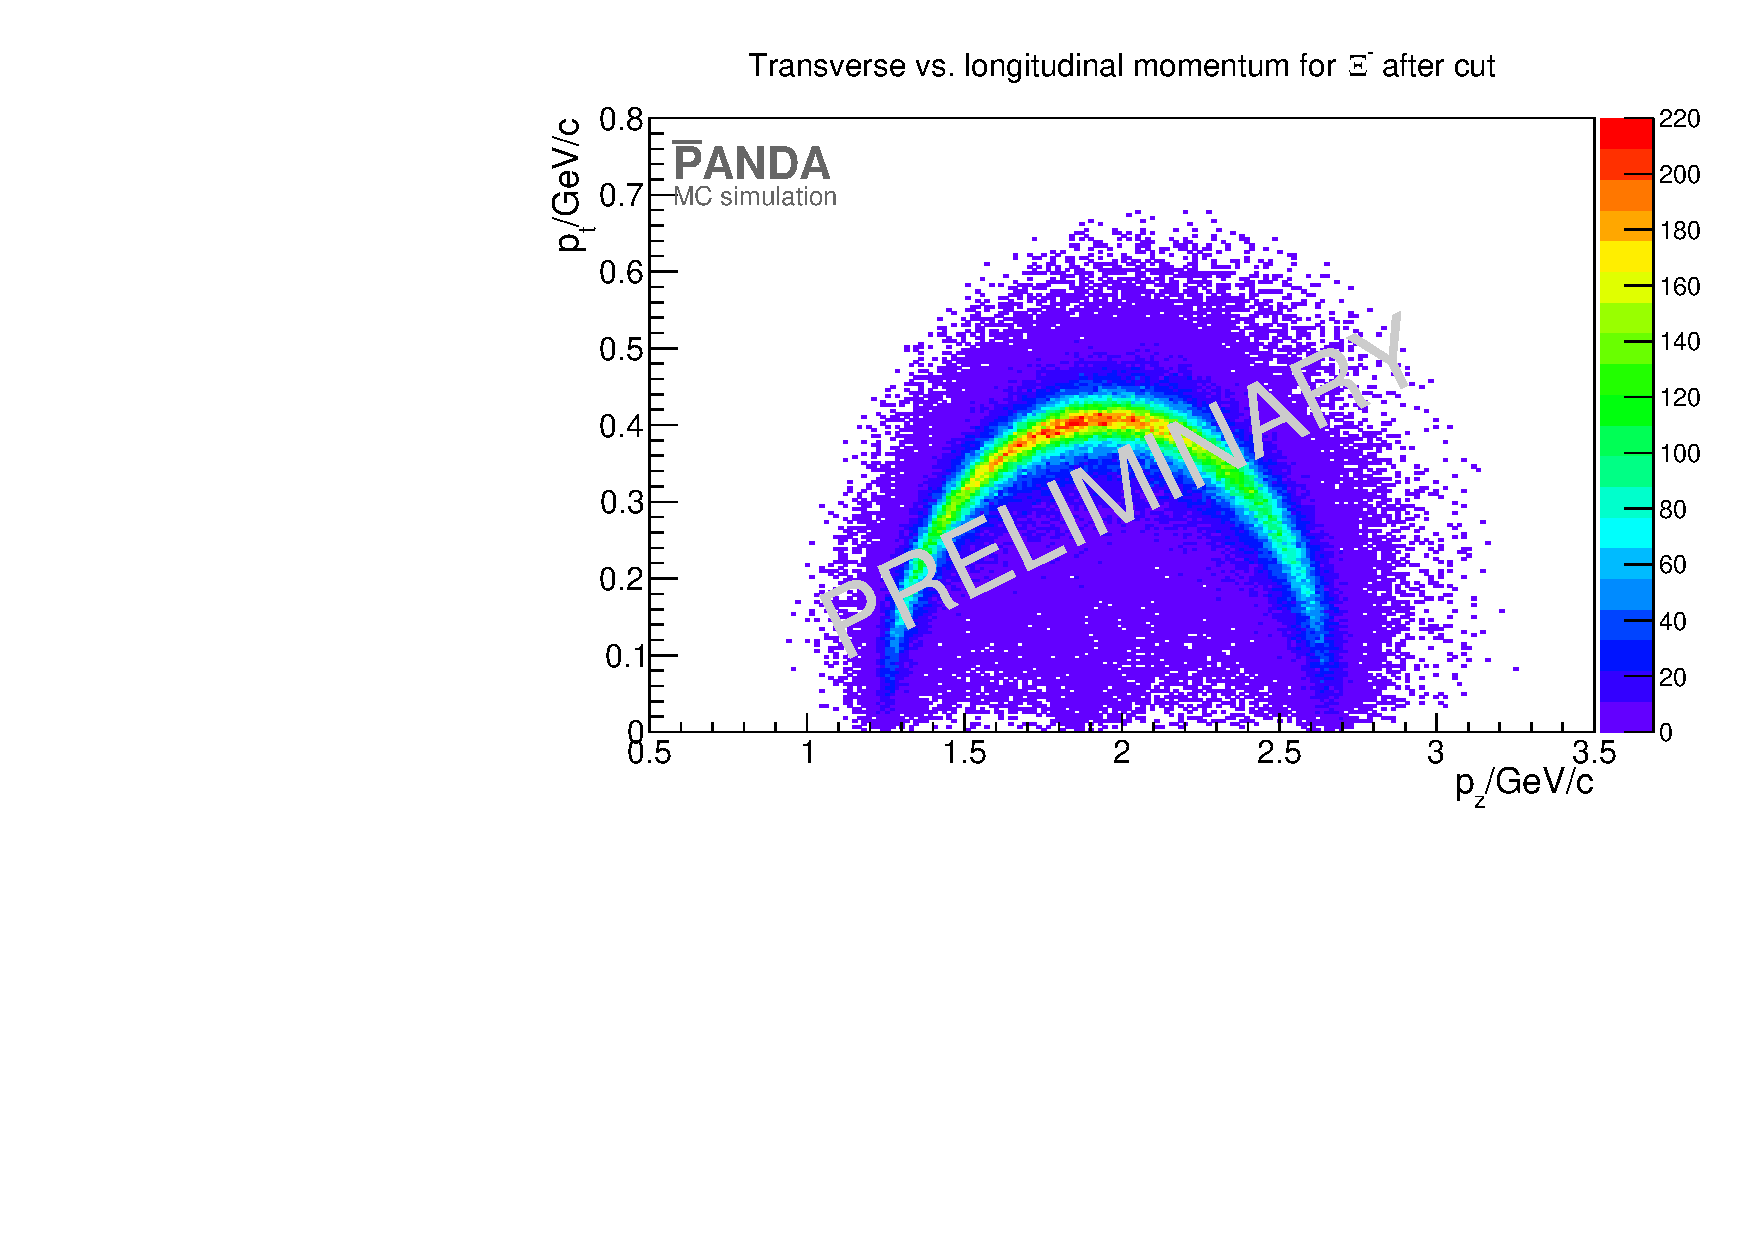
\includegraphics[width=0.49\textwidth]{./plots/Xi/XiMinus_pt_vs_pz_cut.pdf}}
			\caption{\propose The plots shows the transverse against the longitudinal momentum for \anticascade and \cascade}
			\label{fig:XiPlus_pt_vs_pz}
		
		\end{figure}
		
		The reconstruction efficiency for \anticascade is $18.39\%$ and for \cascade $18.64\%$.
		
	
	
	

\section{Reconstruction of $\Xi$(1820) and $\bar{\Xi}$(1820)}
		\subsection*{Selection}

		For the reconstruction of \excitedcascade one combine \lam and \kminus meson and for \excitedanticascade \alam and \kplus using the
		best candidate from \lam and \alam and \kplus and \kminus with more than 3 hits in one of the inner tracking detectors.
		After the combination of the particles a mass window cut with width of $0.3$\massunit is performed. 
		The daughter particles are fitted then to a common vertex point with the PndKinVtxFitter.
		Only those candidates for \excitedcascade (\excitedanticascade) are selected which have a fit probability of more then $1\%$.
		The selection scheme is shown in figure \ref{fig:excitedcascade_scheme}. 
		
		\begin{figure}
			\centering
				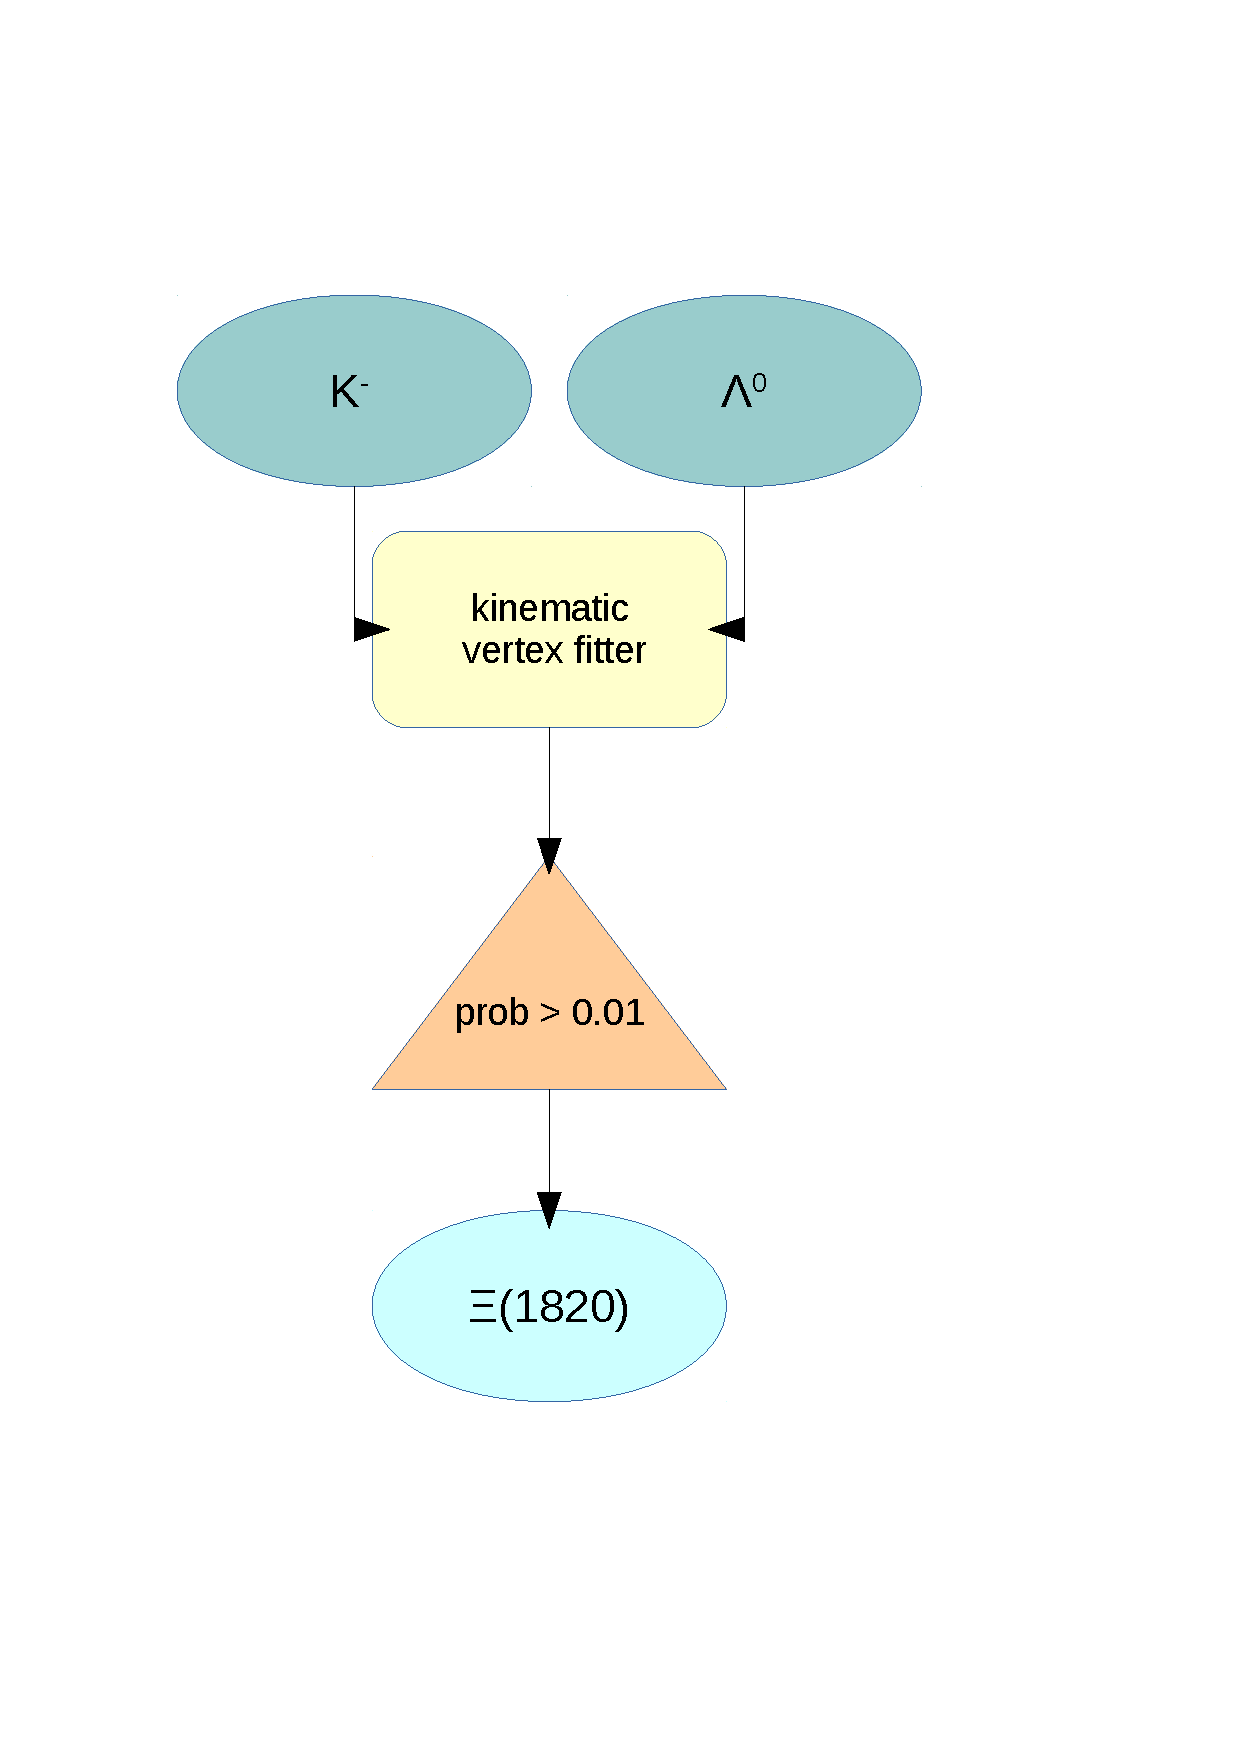
\includegraphics[width=0.50\textwidth]{./plots/combineExcitedCascade.pdf}
			\caption{\propose Scheme for \excitedcascade reconstruction}
			\label{fig:excitedcascade_scheme}
		\end{figure}
		
		
		The \chisq probability distribution for the vertex fit is shown in figure \ref{fig:xi1820_prob}.
		The distribution is again not flat but increases for values up to one. 
		
		\begin{figure}
			\centering
			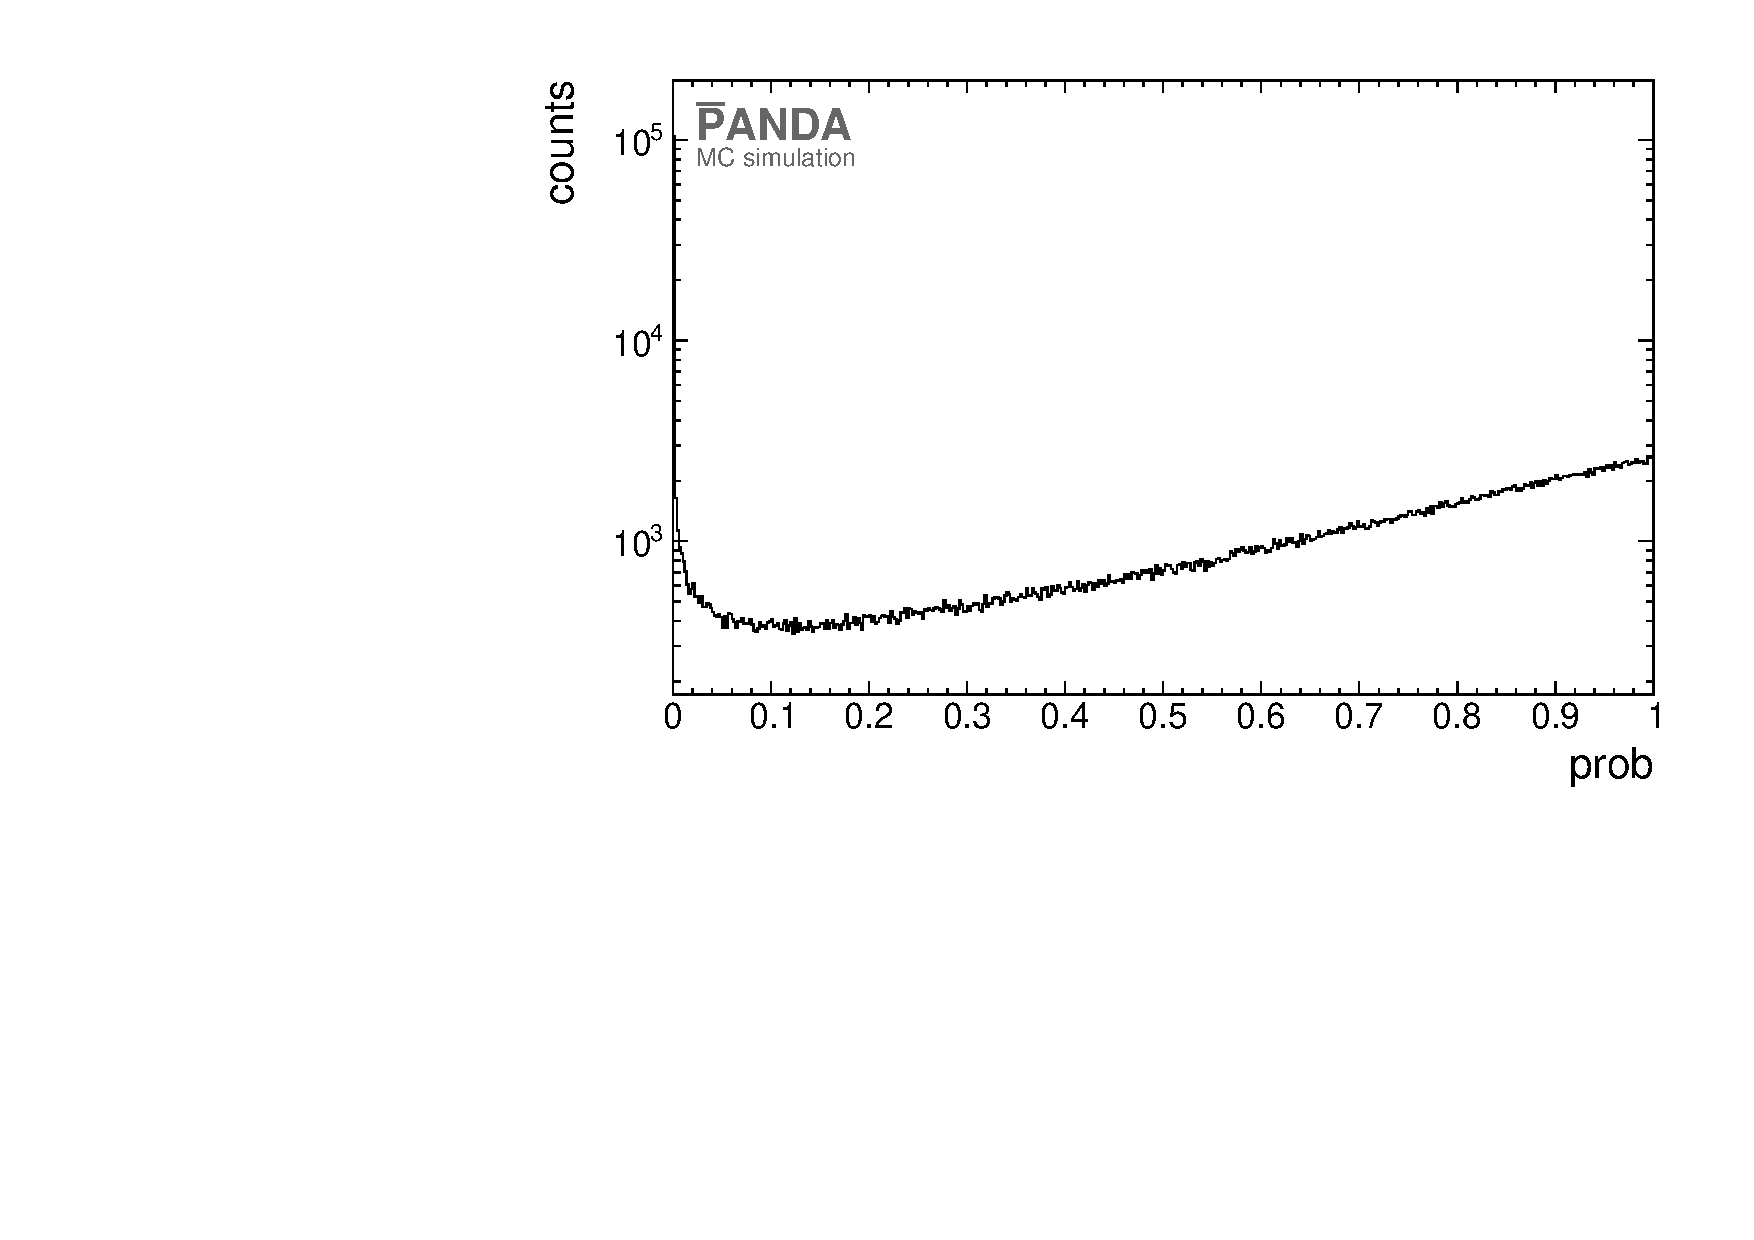
\includegraphics[width=1.\textwidth]{./plots/Xi1820/XiMinus1820_prob.pdf}
			\caption{\propose \chisq probability distribution of kinematic vertex fit for \excitedcascade.}
			\label{fig:xi1820_prob}
		\end{figure}
		
		If there is more than one particle the best candidate is chosen.
		
	\subsection*{Results}
	The vertex resolution for \excitedcascade and \excitedanticascade is summarized in table \ref{tab:Xi1820_vtxres}.
	
	\begin{table}
		\centering
		\caption{\propose Vertex resolution for \excitedcascade and \excitedanticascade.}
		\label{tab:Xi1820_vtxres}
		\begin{tabular}{ccc}
			\hline
			position & \excitedcascade & \excitedanticascade (from c.c.) \\
			\hline
			\hline
			x/cm & 0.028 & 0.028\\
			y/cm & 0.028 & 0.028\\
			z/cm & 0.1 & 0.1\\
			\hline
			 
		\end{tabular}
	\end{table}
	
	Here again the vertex resolution is calculated with the FWHM. 
	This is exemplarily shown for \excitedcascade in figure \ref{fig:Xi1820_vtxx} and figure \ref{fig:Xi1820_vtxyz}.
	
	\begin{figure}
		\centering
		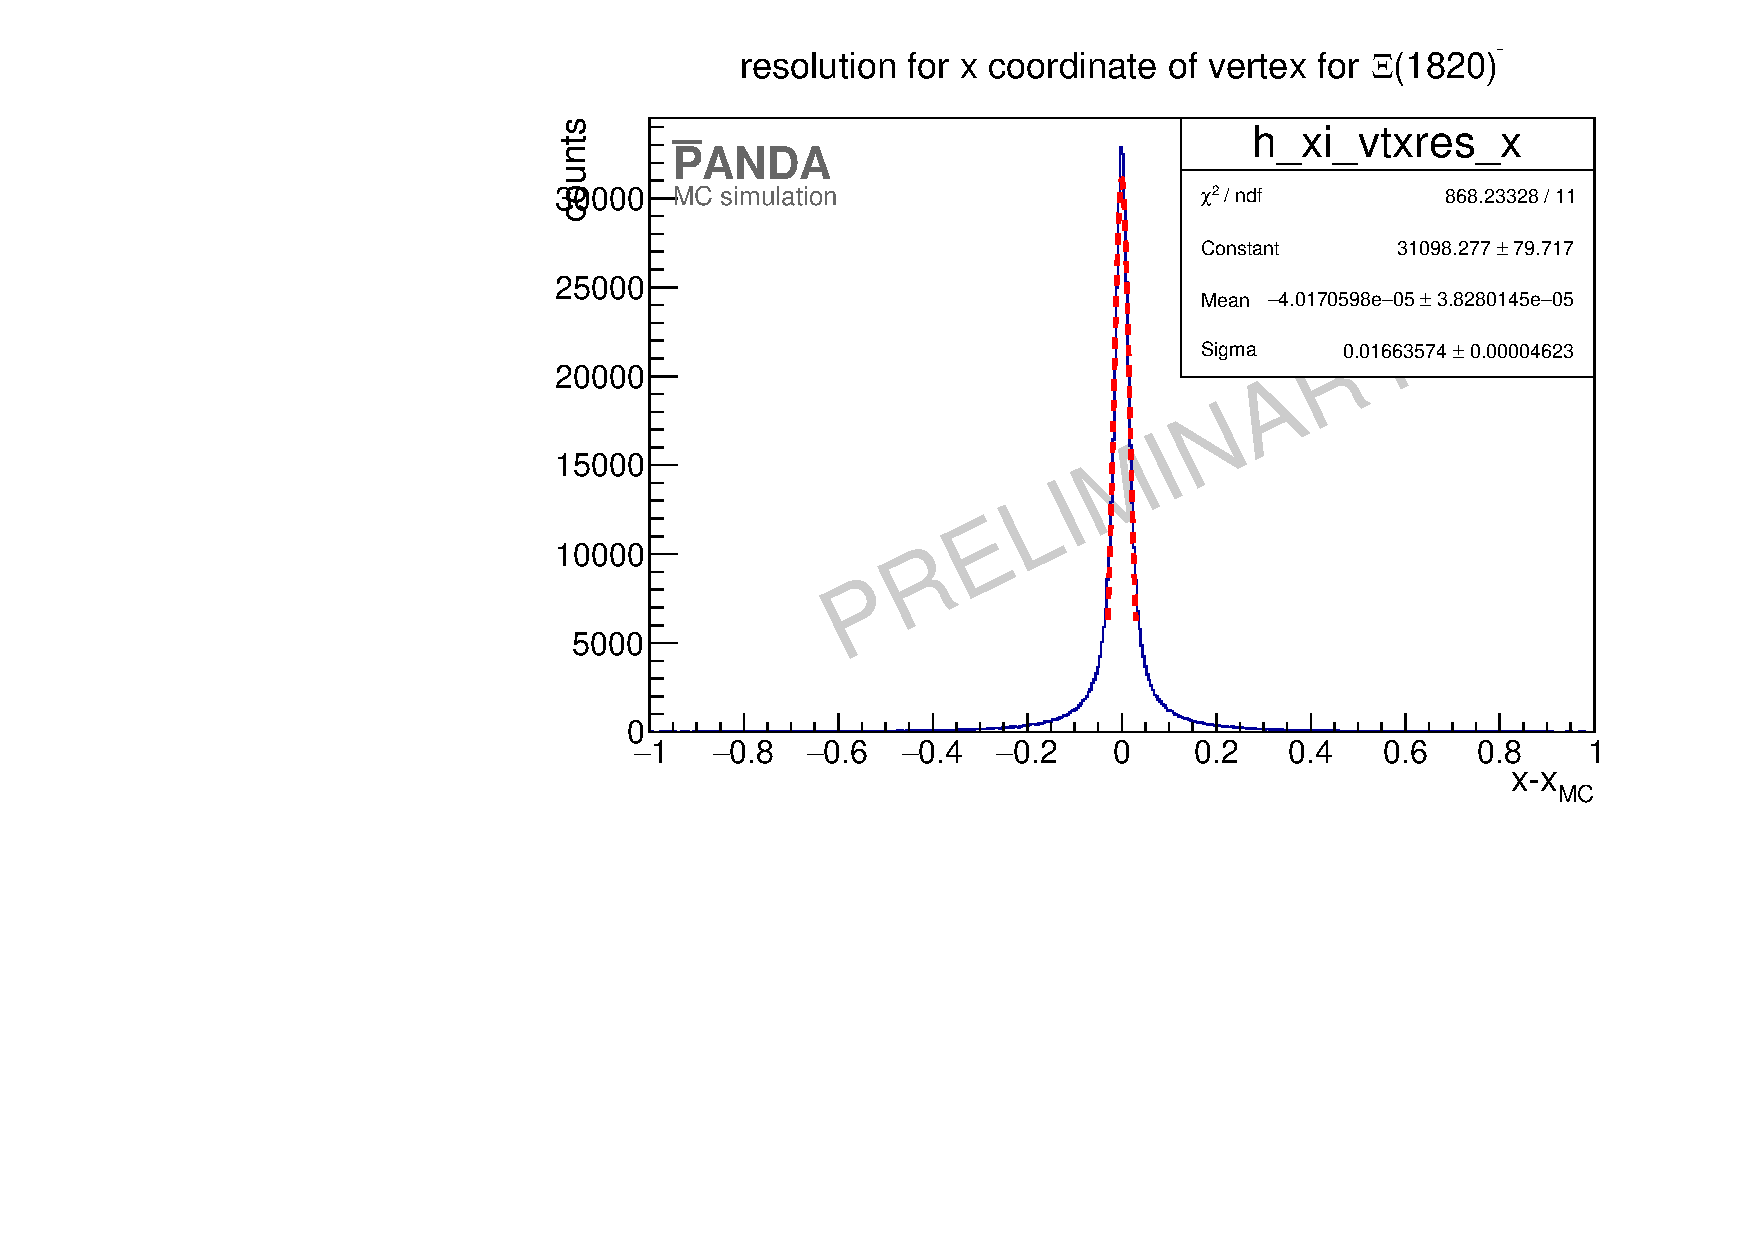
\includegraphics[width=0.7\textwidth]{./plots/Xi1820/XiMinus1820_vtxres_x.pdf}
		\caption{\propose Vertex resolution of the x coordinate for \excitedcascade.}
		\label{fig:Xi1820_vtxx}
	\end{figure}
	
	 \begin{figure}
		\centering
		\subfigure[Vertex resolution of the y coordinate for \excitedcascade.]{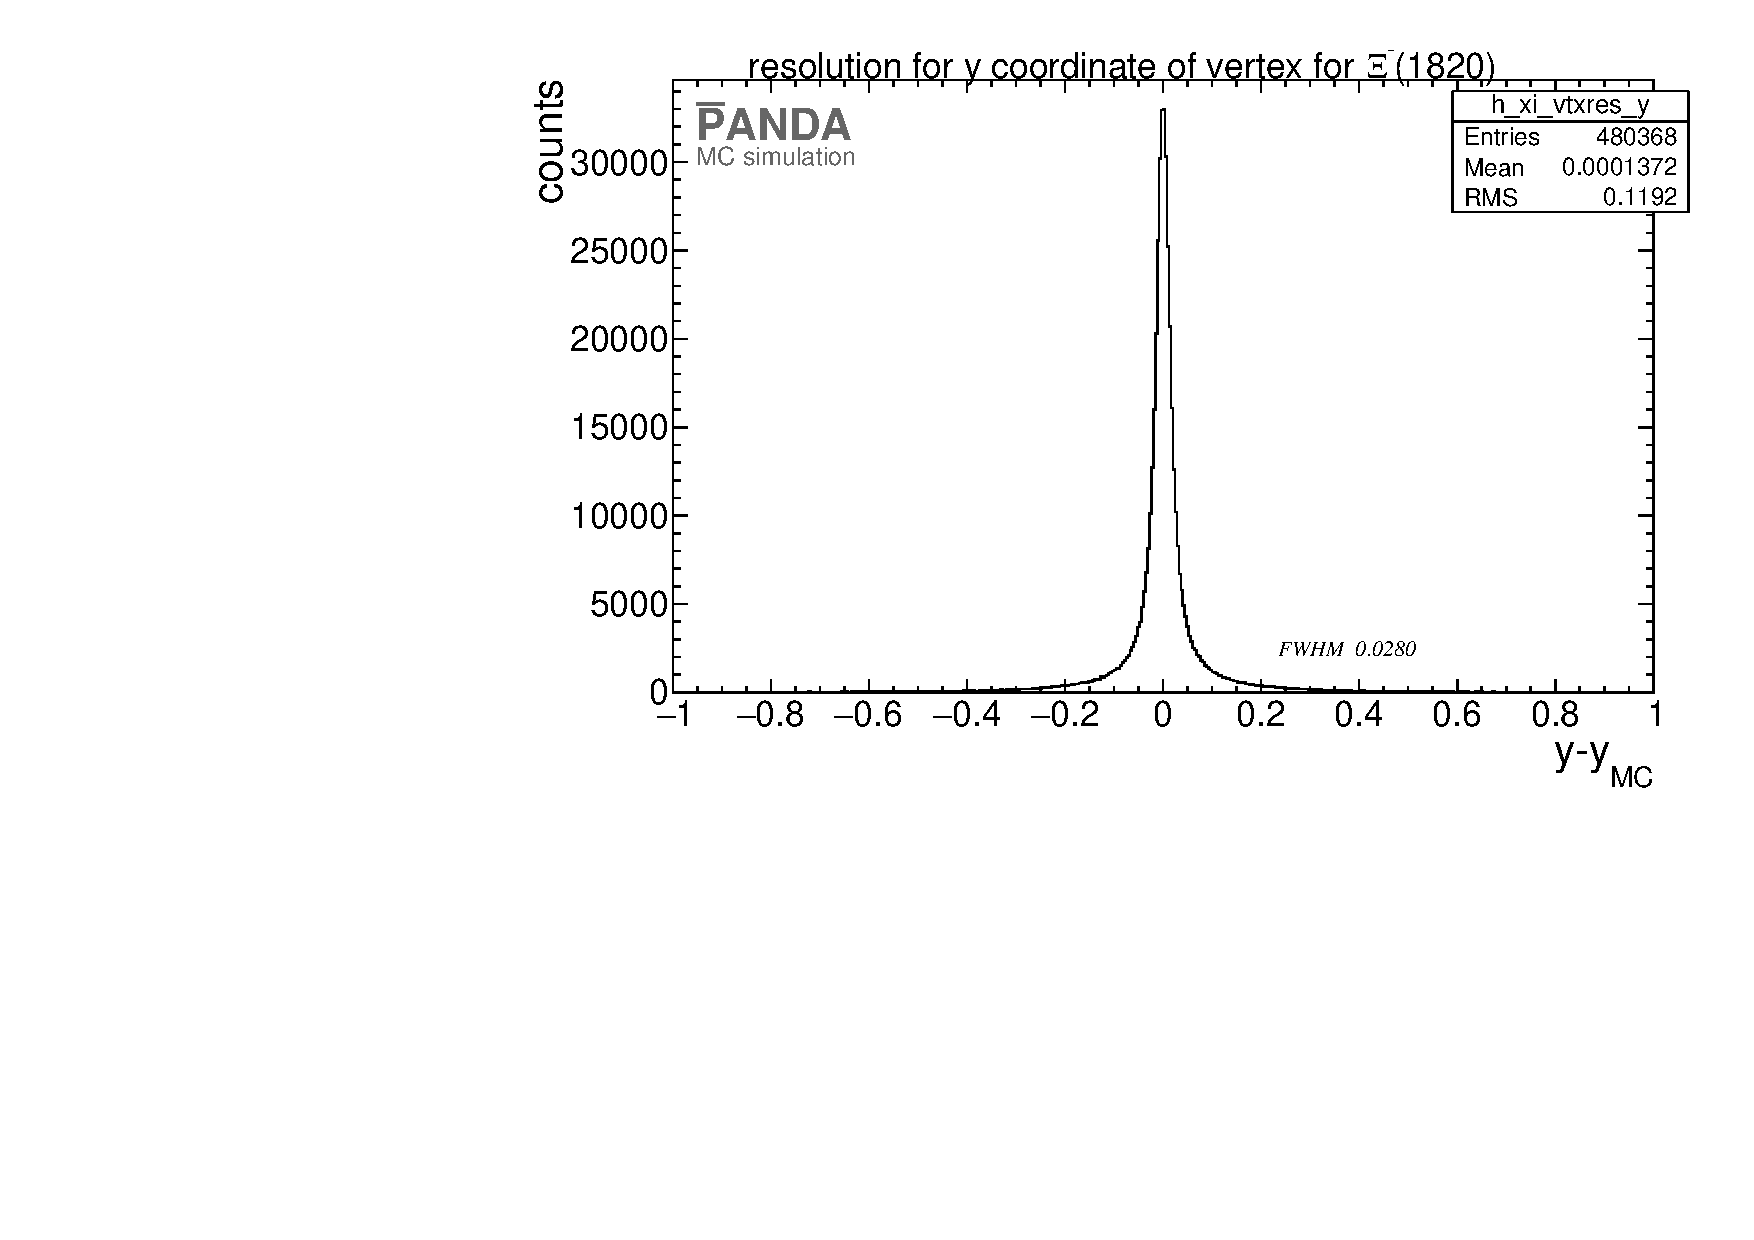
\includegraphics[width=0.49\textwidth]{./plots/Xi1820/XiMinus1820_vtxres_y.pdf}}
		\subfigure[Vertex resolution of the z coordinate for \excitedcascade.]{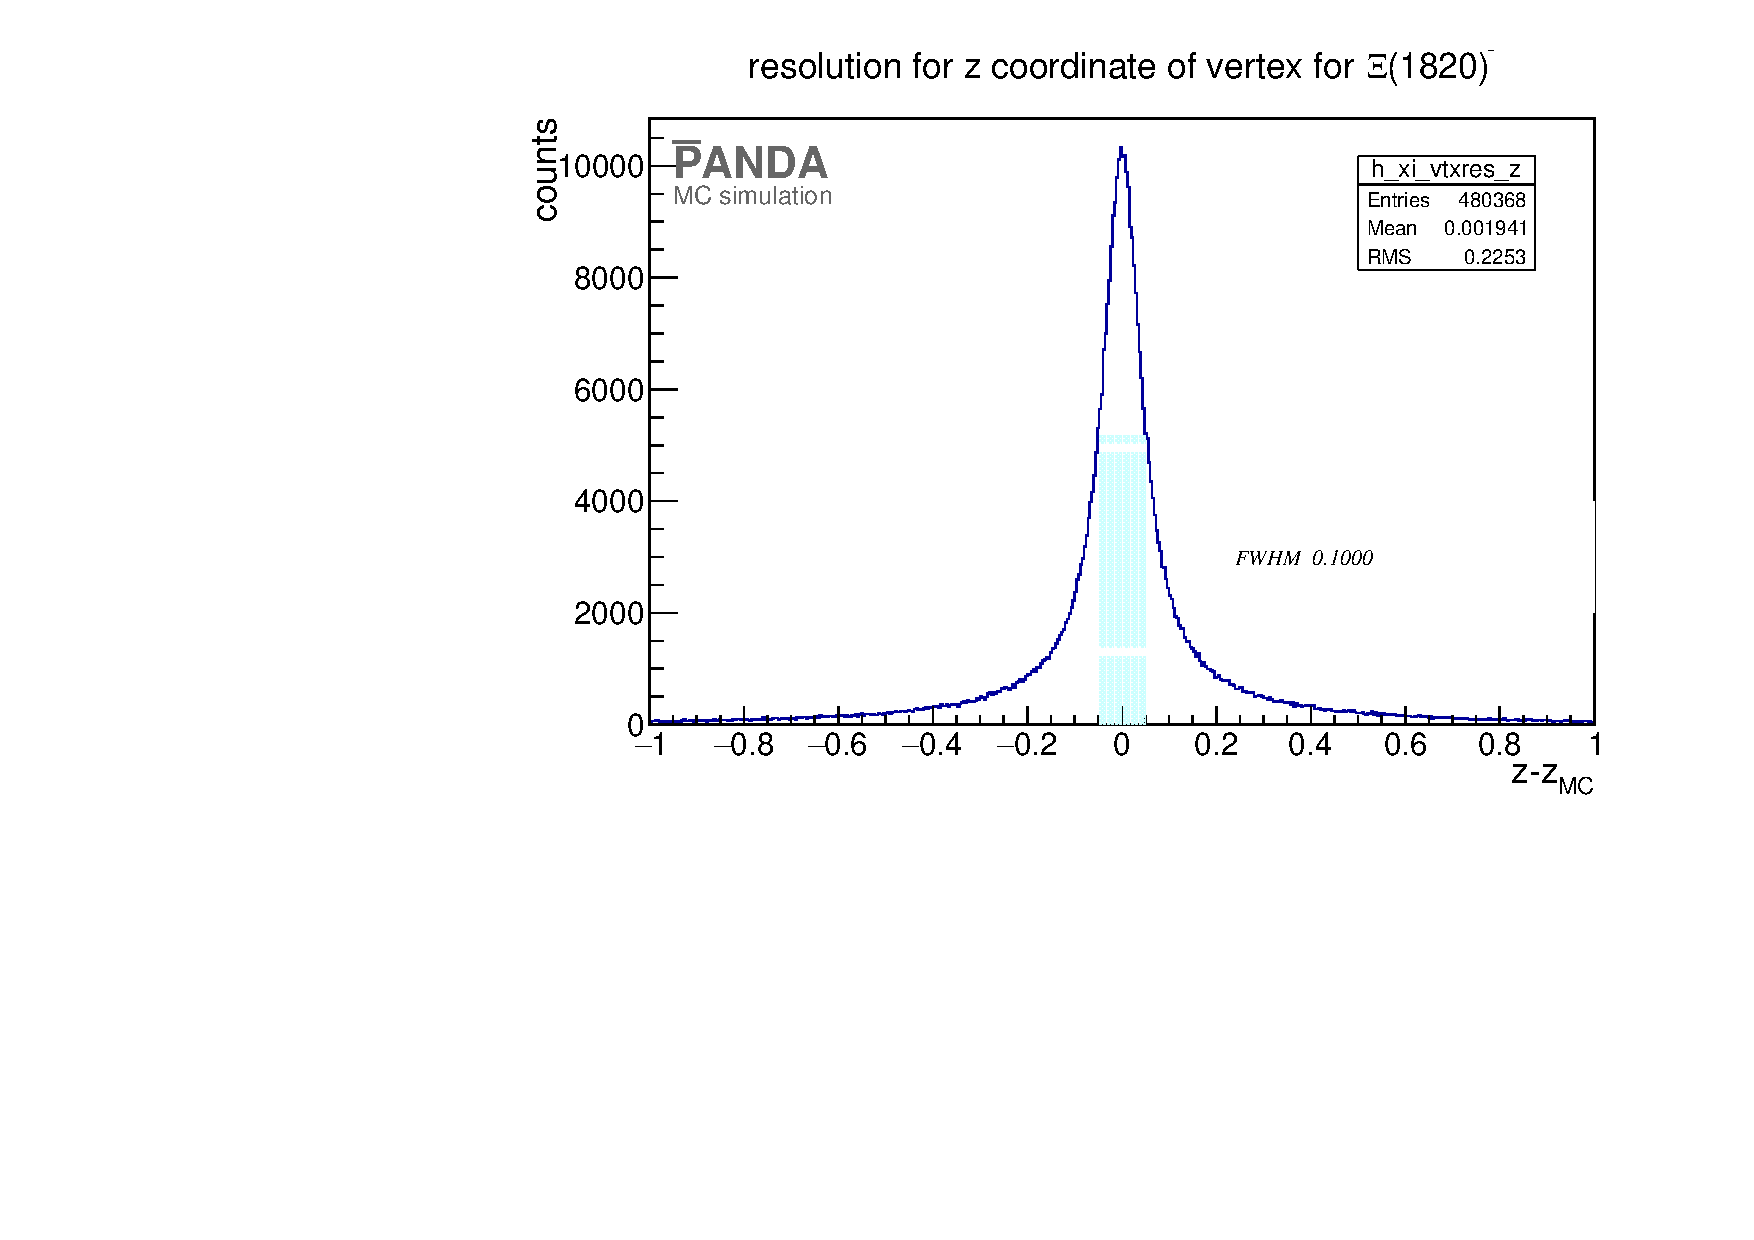
\includegraphics[width=0.49\textwidth]{./plots/Xi1820/XiMinus1820_vtxres_z.pdf}}
		\caption{\propose Figure a) shows the vertex resolution for the y coordinate and figure b) for the z coordinate of \excitedcascade}
		\label{fig:Xi1820_vtxyz}
	\end{figure}
	
	After performing the both fits and cut on the probability values, the mass for \excitedcascade and \excitedanticascade
	can be determined by fitting the mass with a double Gaussian fit. 
	Figure \ref{fig:xi1820_mass_diffcuts} shows the mass distribution for both particles after each cut.
	
	\begin{figure}
		\centering
		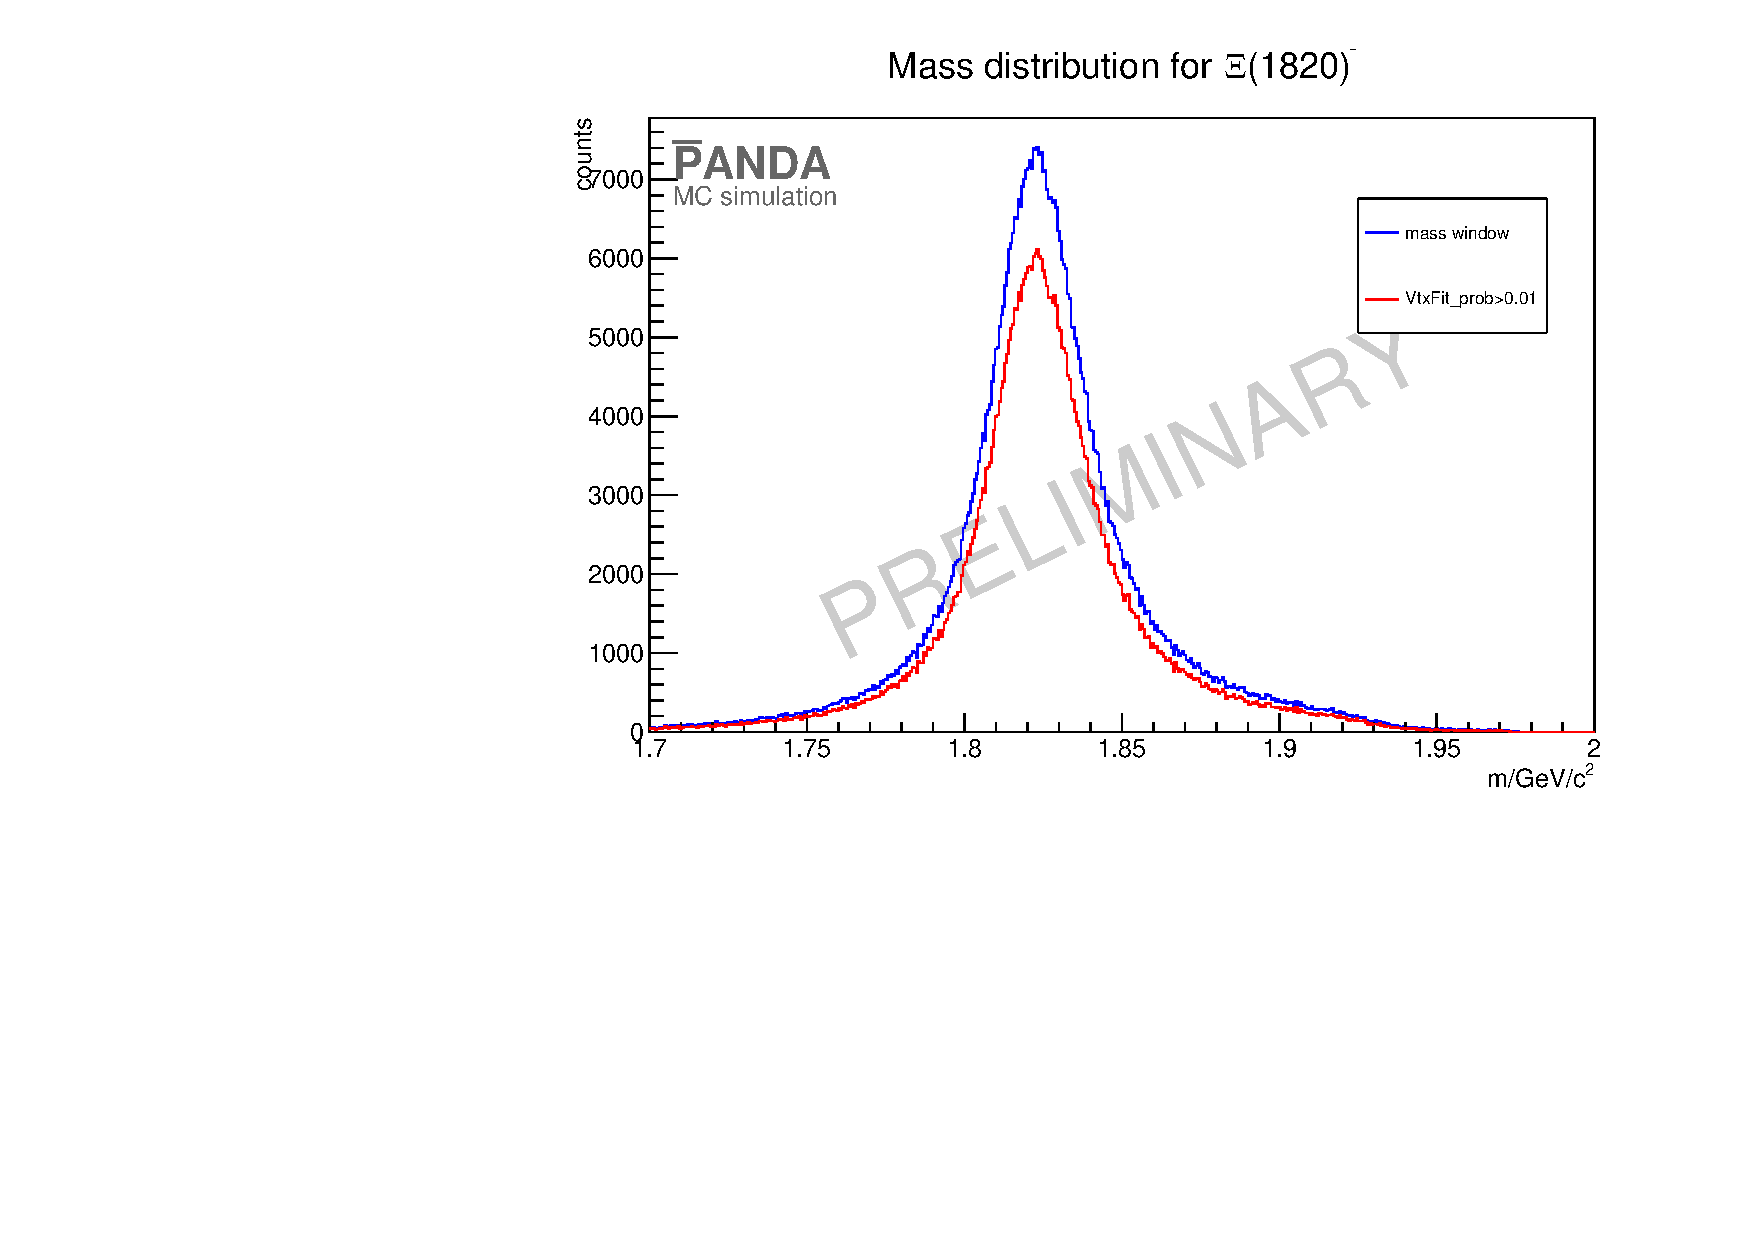
\includegraphics[width=1.\textwidth]{./plots/Xi1820/XiMinus1820_m_diffcuts.pdf}
		\caption{\propose Mass distribution for \excitedcascade for the different cuts}
		\label{fig:xi1820_mass_diffcuts}
	
	\end{figure}
	The mass fit is exemplarily shown for the \excitedcascade in figure \ref{fig:xi1820_massfit}. 
	
	\begin{figure}
		\centering
		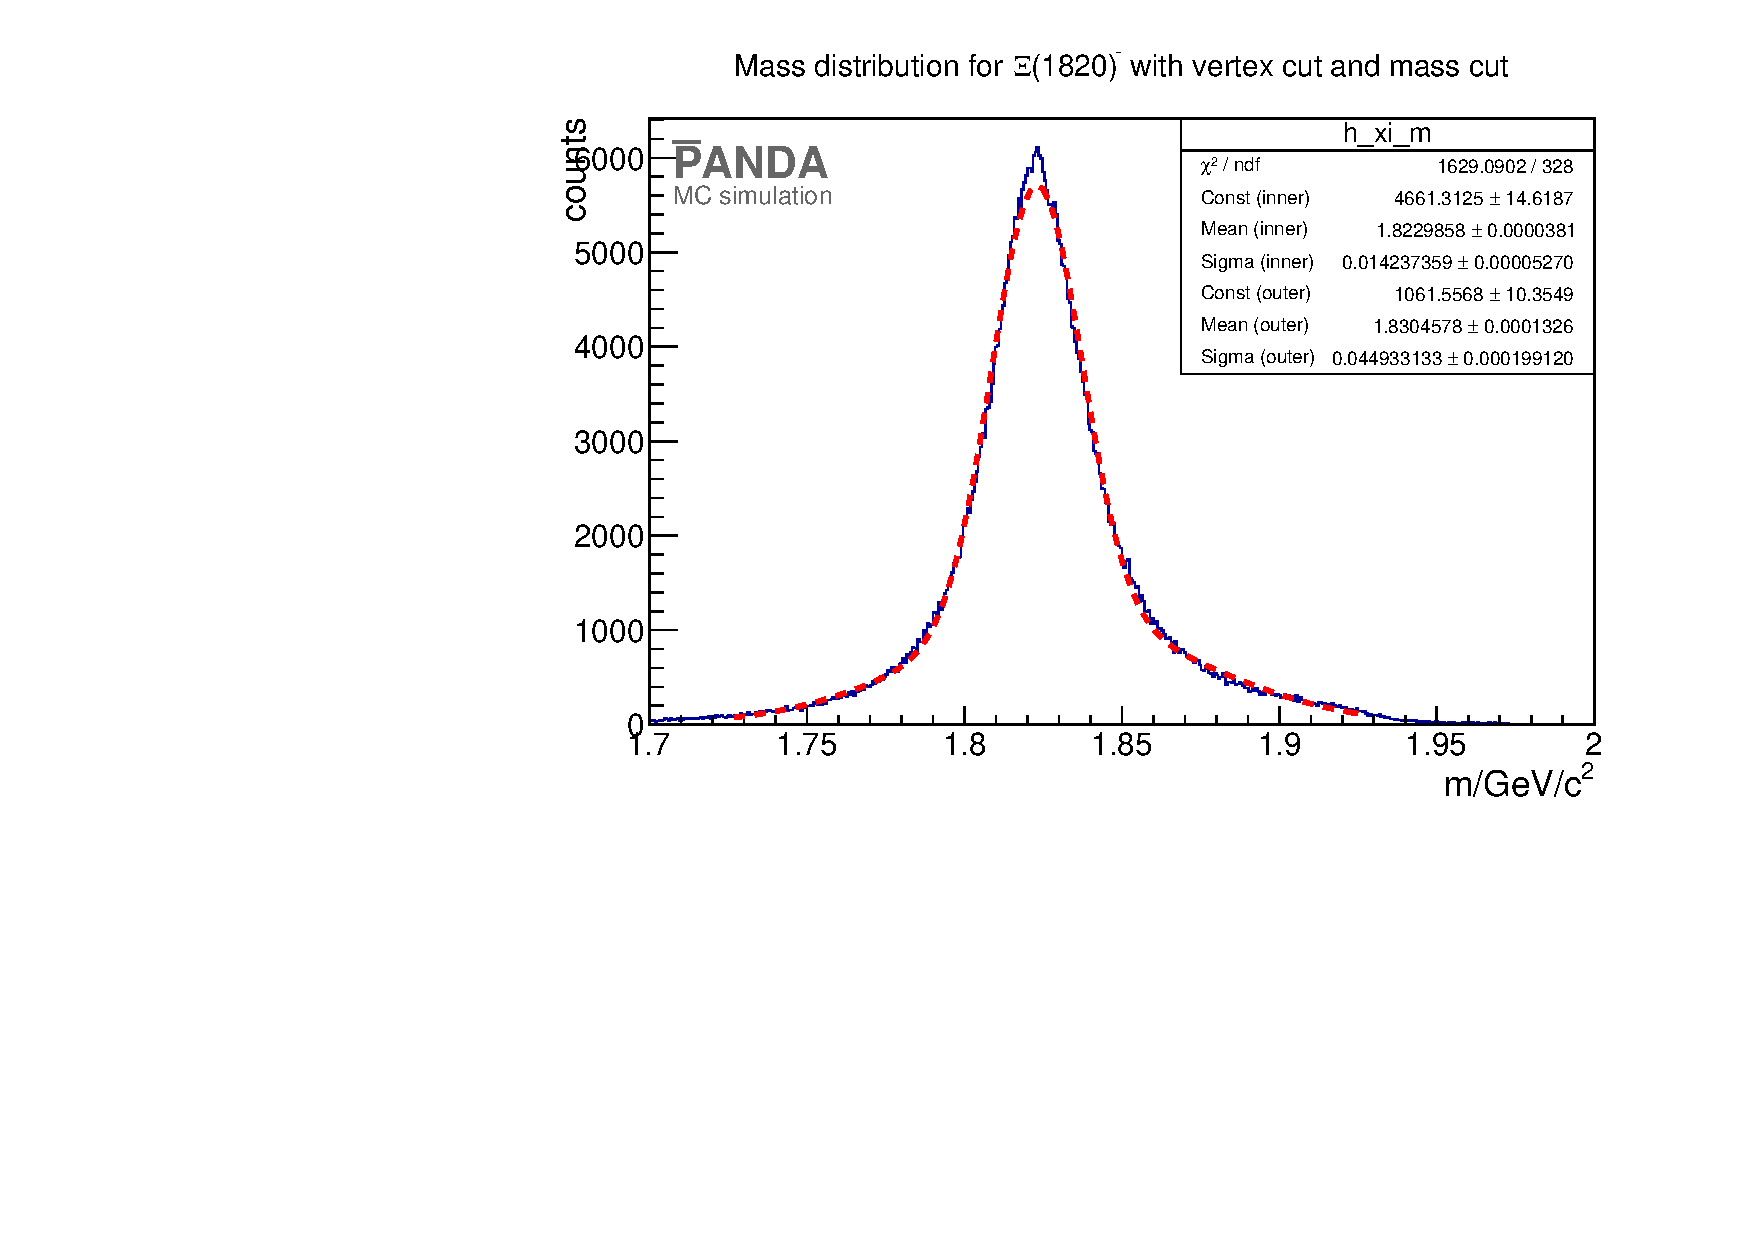
\includegraphics[width=1.\textwidth]{./plots/Xi1820/XiMinus1820_m_masscut.pdf}
		\caption{\propose Mass distribution after all cuts for \excitedcascade.}
		\label{fig:xi1820_massfit}
	\end{figure}
	The mass values for the \excitedcascade is fitted to $1 \pm 1$\massunit and for \excitedanticascade to $1 \pm 1 $\massunit.
	These values are close to the input value.
	Figure \ref{fig:xi1820_pt_vs_pz} shows the two dimensional momentum distribution. For both subplots the x axis shows the longitudinal momentum
	and on the y axis there is shown the transverse momentum.
	
	\begin{figure}
		\centering
		\subfigure[\excitedcascade]{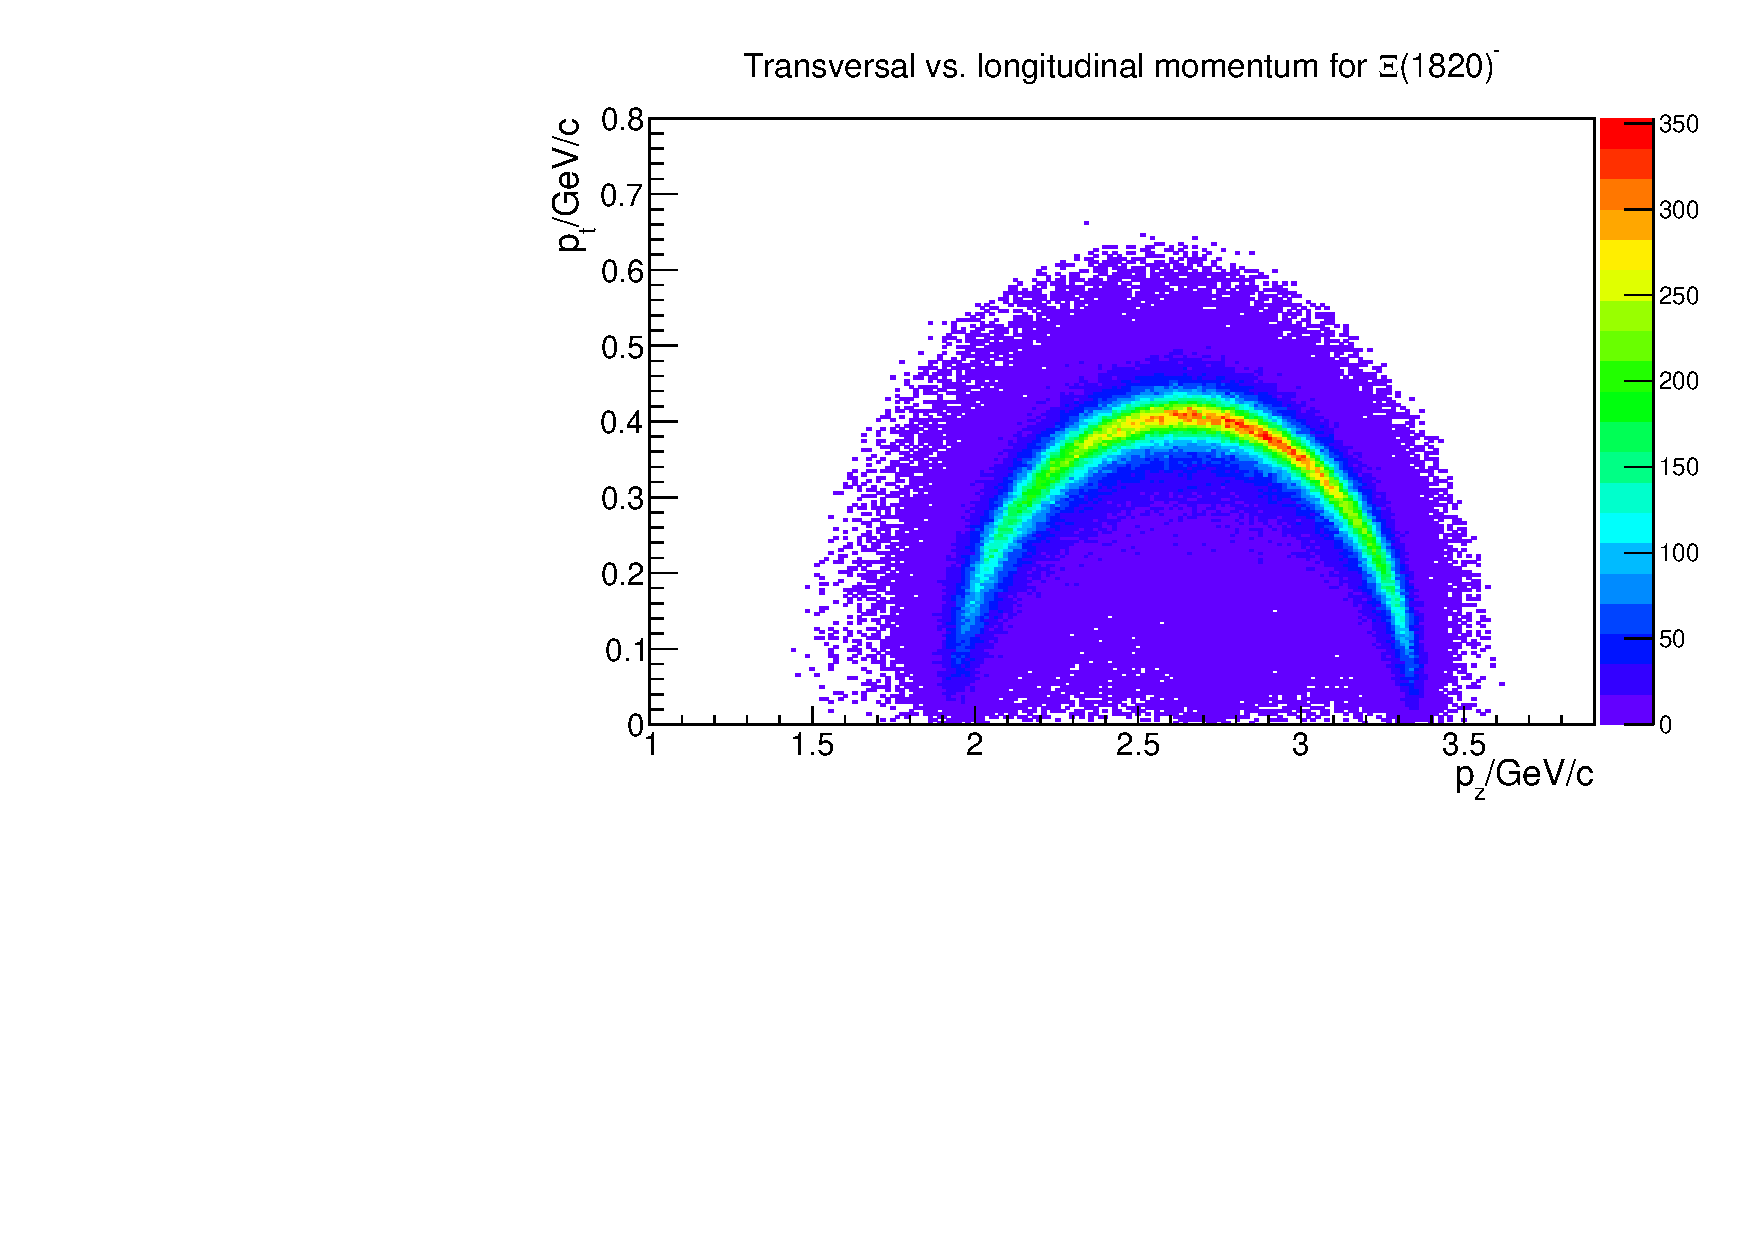
\includegraphics[width=0.49\textwidth]{./plots/Xi1820/XiMinus1820_pt_vs_pz_cut.pdf}}
		\subfigure[\excitedanticascade]{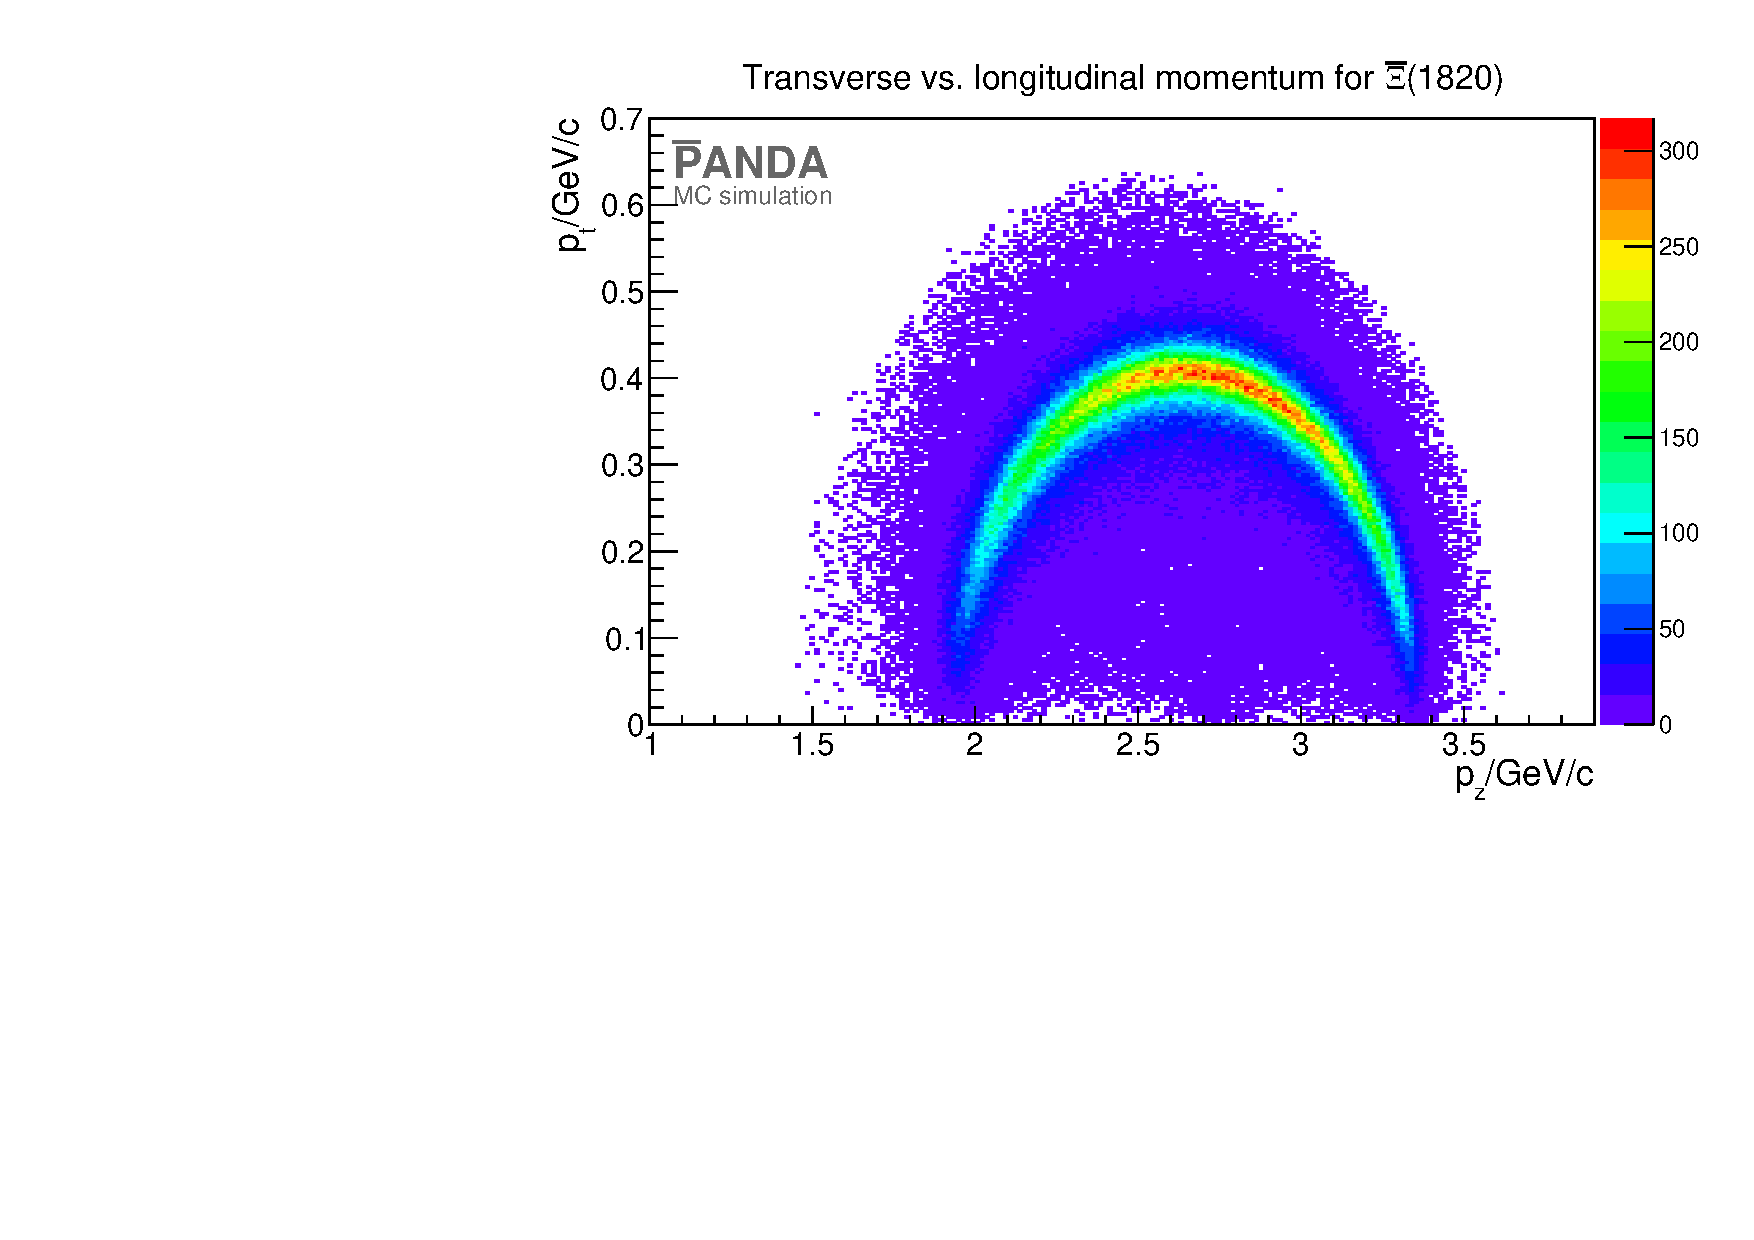
\includegraphics[width=0.49\textwidth]{./plots/Xi1820/XiPlus1820_pt_vs_pz_cut.pdf}}
		\caption{\propose Both plots show the longitudinal versus the transverse momentum of the excited cascade baryon.}
		\label{fig:xi1820_pt_vs_pz}
	\end{figure}
	
	The reconstructed distributions are in good agreement with the distribution coming from the simulated events which are 
	shown in figure \ref{fig:MC_xi_pt_vs_pz} (b).
	
\section{Reconstruction of hole chain}

	\subsection*{Selection}
	
	To reconstruct the hole reaction chain \excitedcascade and \anticascade are combined.
	This is also done with \excitedanticascade and \cascade for the charge conjugated channel.
	For the event selection now it is use a excluding method. 
	The four momentum vector of the daughter particles is fitted to the initial for momentum vector  

	\begin{center}
		\begin{equation}\nonumber
			\left(\mt{p}_x,\, \mt{p}_y,\, \mt{p}_z,\, \mt{E} \right) = \left(0,\, 0,\, 4.6,\, 5.63 \right)
		\end{equation}
	\end{center}
	of the \pbarpSystem.	
	This fit is performed with the PndKinFitter.
	After the four momentum fit there were only those candidates selected which have a \chisq probability of more than $1\%$.
	The \chisq probability is shown in figure \ref{fig:xisys_prob}. 
	The red line denotes the cut value.

	\begin{figure}
		\centering
		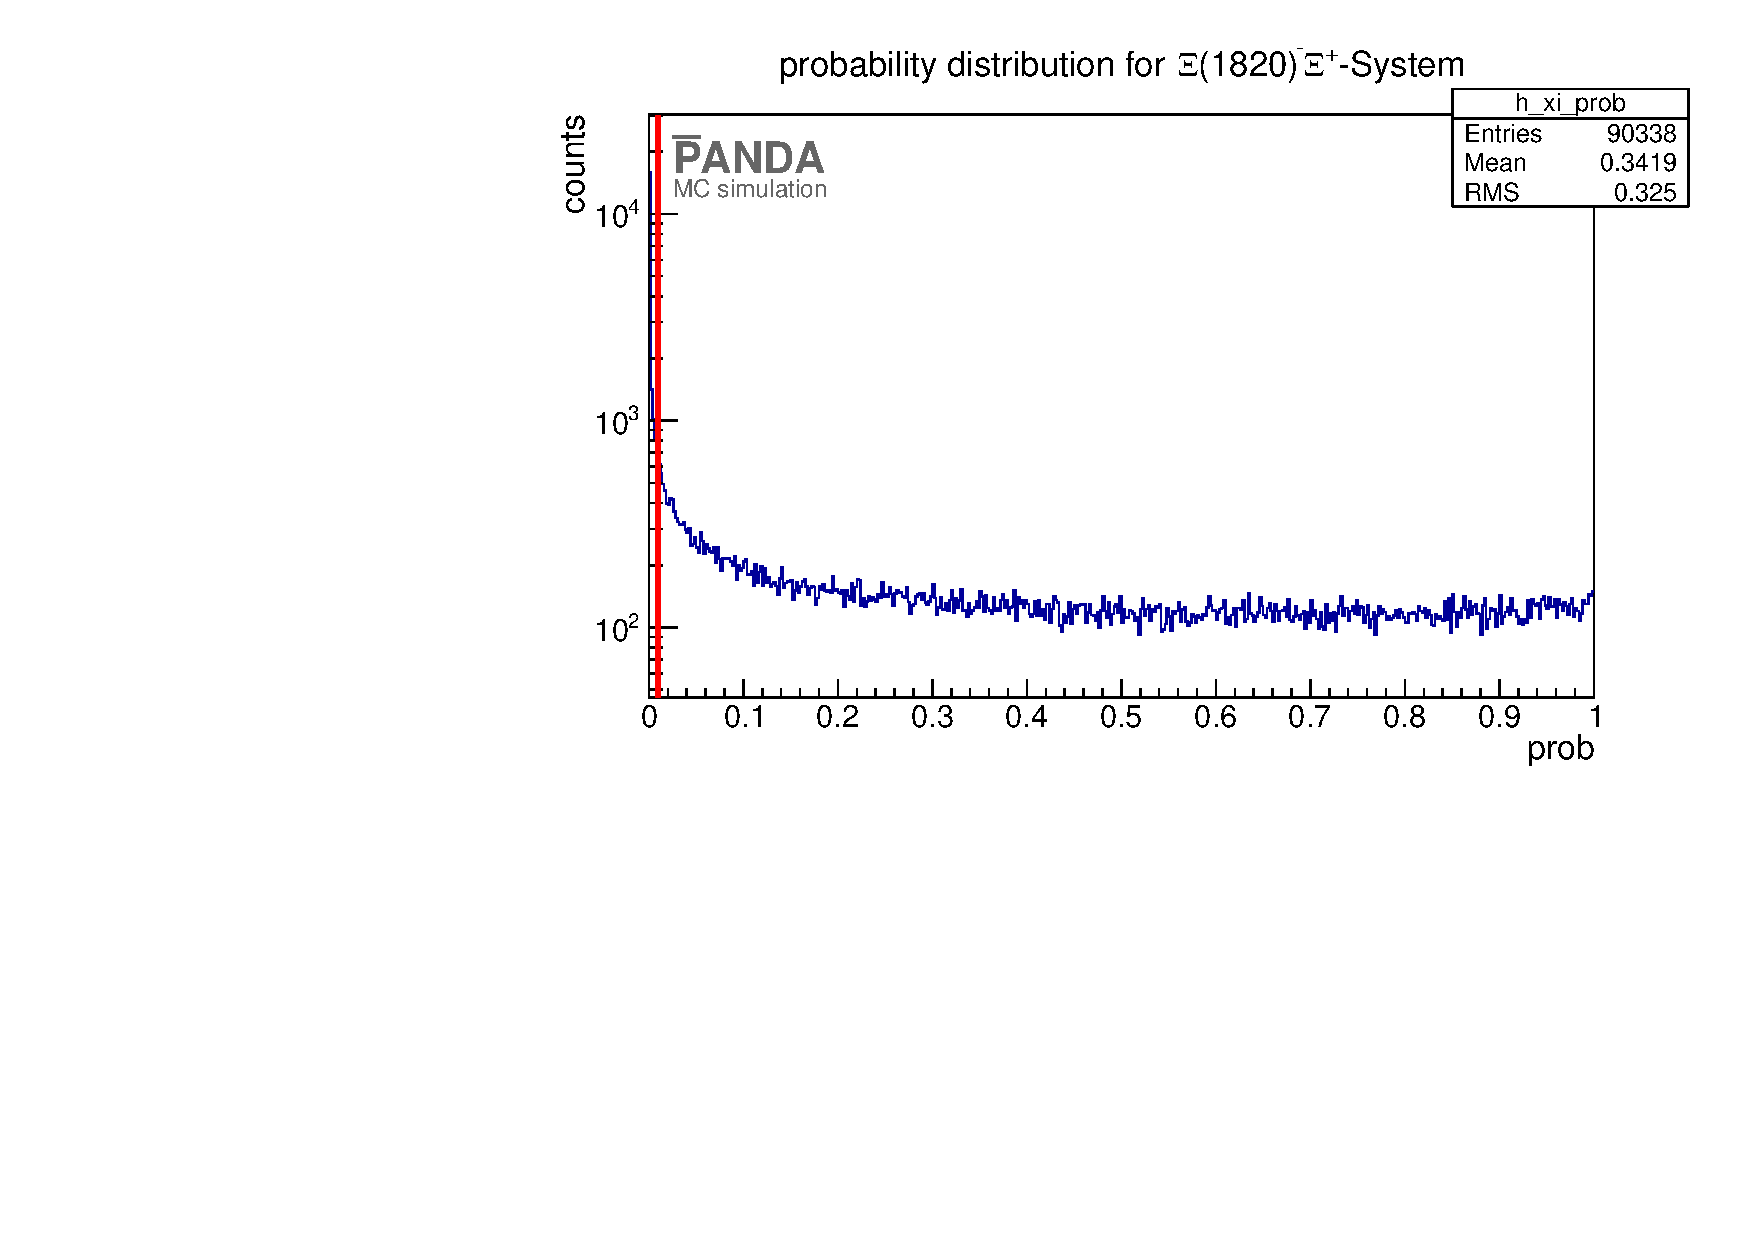
\includegraphics[width=0.7\textwidth]{./plots/pbarp/XiSys_prob.pdf}
		\caption{\propose 4-constraint fit probability}
		\label{fig:xisys_prob}
	\end{figure}
	
	The selection scheme is shown in figure \ref{fig:fourconstraintfit}
	 
	\begin{figure}
		\centering
			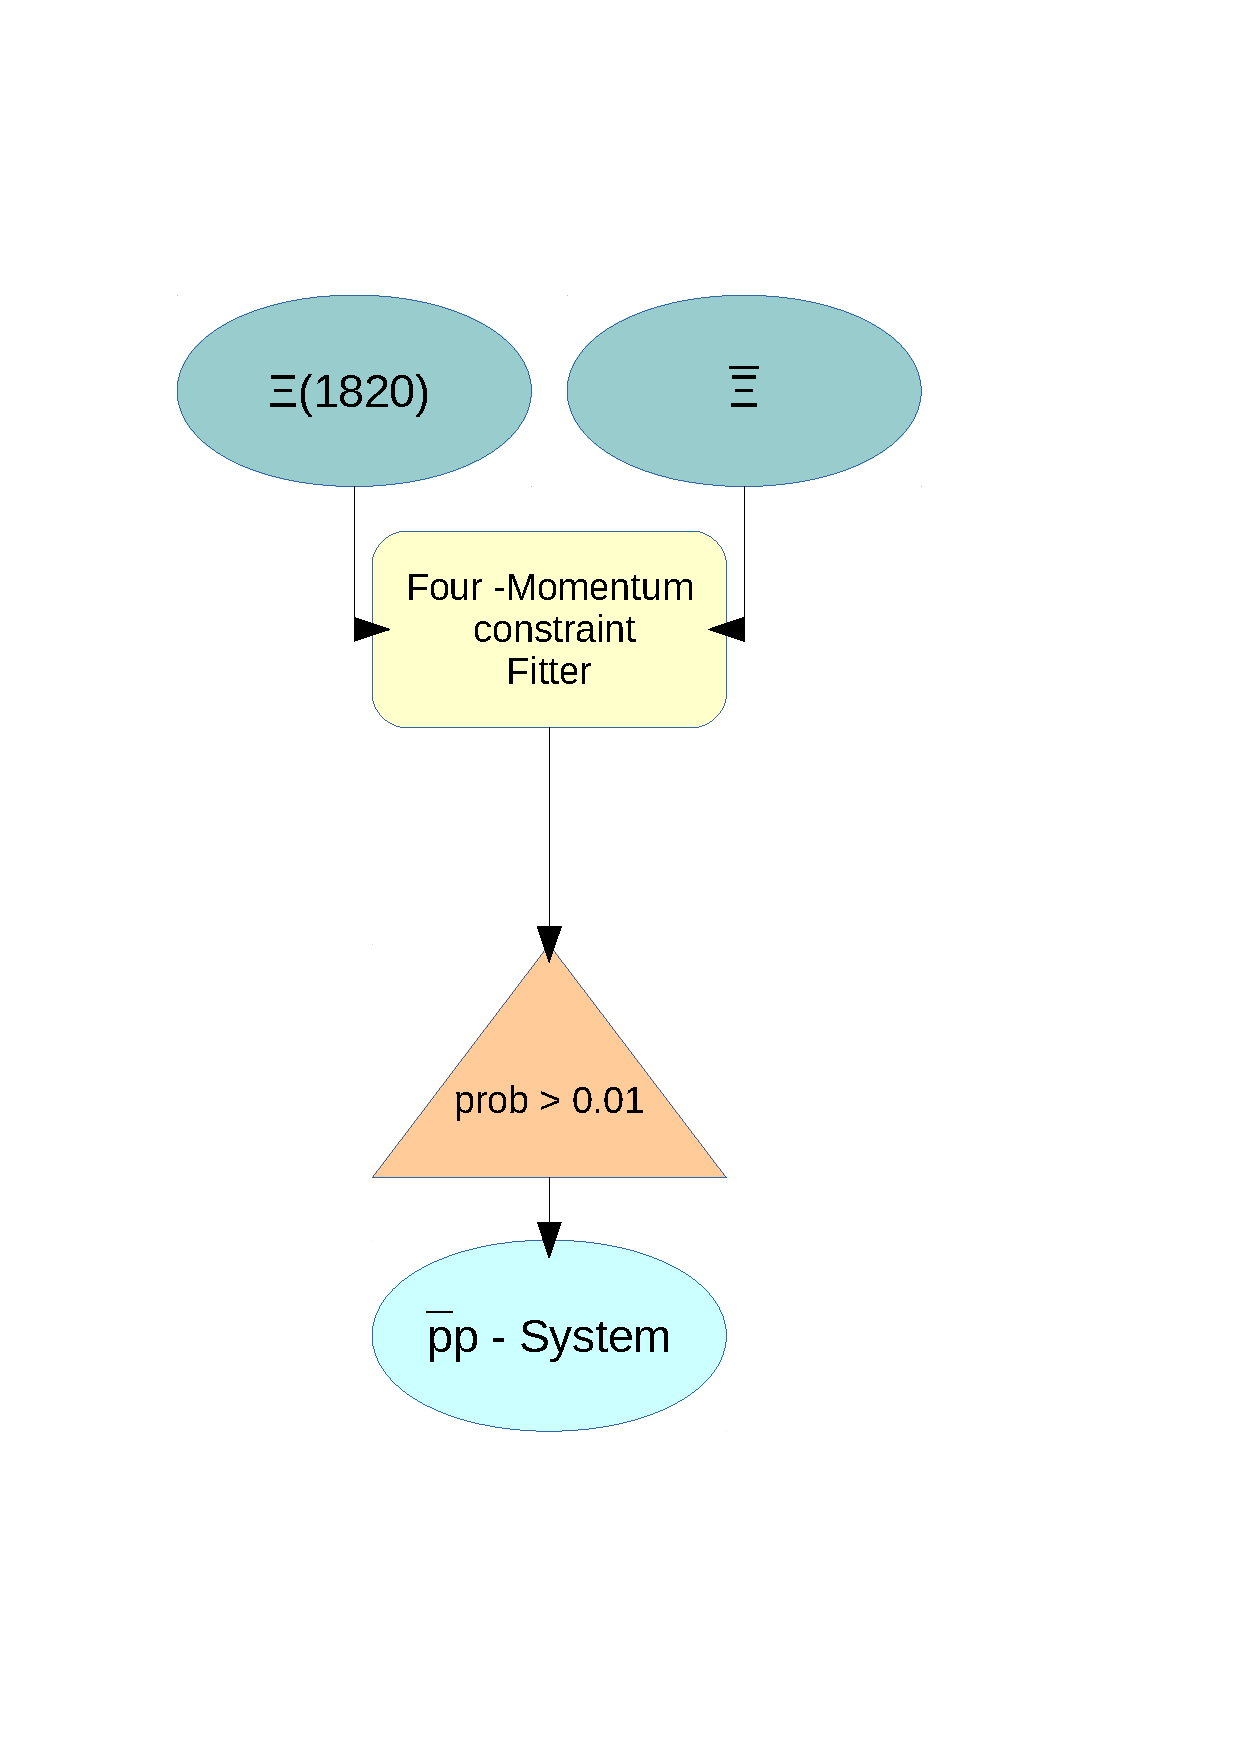
\includegraphics[width=0.50\textwidth]{./plots/combineCascadeSys.pdf}
		\caption{\propose Scheme for 4-Constraint Fit}
		\label{fig:fourconstraintfit}
	\end{figure}
	
	\subsection*{Results}
	
	The results of the reconstruction efficiency for all non-final state particles is shown in table \ref{tab:non-finalstate_efficiency}
	and table \ref{tab:non-finalstate_efficiency_cc}.
	
	\begin{table}
		\centering
		\caption{\propose reconstruction efficiency for non-final state particles for \pbarpSystem $\rightarrow$ \excitedcascade \anticascade}
		\label{tab:non-finalstate_efficiency}
		
		\begin{tabular}{lcc}
		
			\hline
			particle & reco efficiency in $\%$ & dp/p in $\%$ \\\hline
			\hline
			\lam & 50.3278&   1.50497 \\
			\alam & 41.4625&   1.45024\\
			\anticascade & 18.389&   1.2889\\
			\excitedcascade & 32.0245&   2.67691 \\
			\excitedcascade \anticascade system & 4.69293&   1.03214\\\hline
			 	
		\end{tabular}
	\end{table}
	
		\begin{table}
		\centering
		\caption{\propose reconstruction efficiency for non-final state particles for \pbarpSystem $\rightarrow$ \excitedanticascade \cascade}
		\label{tab:non-finalstate_efficiency_cc}
		
		\begin{tabular}{lcc}
		
			\hline
			particle & reco efficiency in $\%$ & dp/p in $\%$ \\\hline
			\hline
			\lam & 42.4693&   1.45429 \\
			\alam & 48.9991&   1.50196\\
			\cascade & 18.6405&   2.29877\\
			\excitedanticascade & 33.2238&   1.31081\\
			\excitedanticascade \cascade system & 4.87227&   1.03127\\\hline
			 	
		\end{tabular}
	\end{table}
	
	How good the reconstruction works is shown in figure \ref{fig:reco_Dalitzplot}.
	This plot shows the Dalitz plot for the \anticascade, \lam and \kminus final states after the reconstruction. 
	Compared with the Dalitz plot of the simulated particles which is shown in figure \ref{fig:eventgeneration_Dalitz} the reconstruction seems to be good.
	
	\begin{figure}
		\centering
		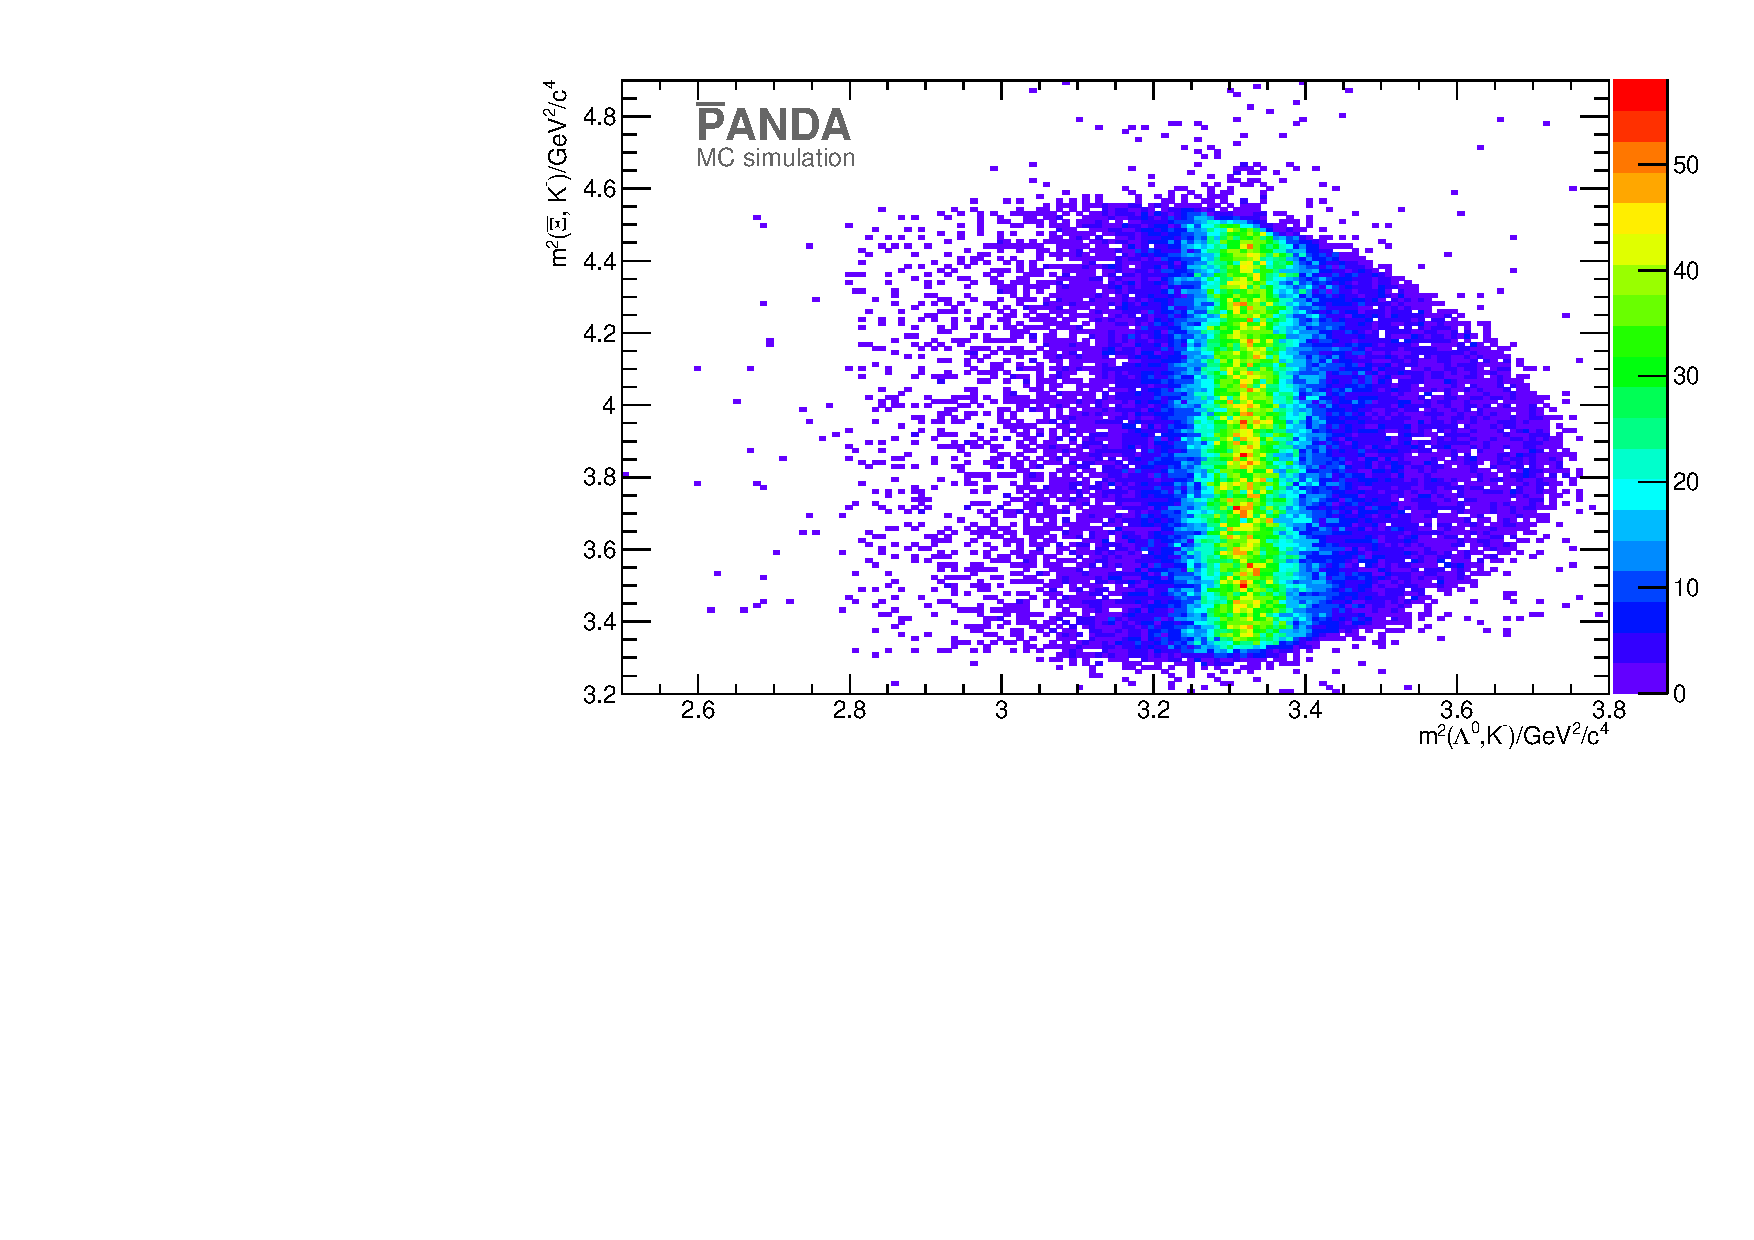
\includegraphics[width=0.8\textwidth]{./plots/pbarp/Dalitzplot_reco.pdf}
		\caption{\propose Dalitz plot for reconstructed particles}
		\label{fig:reco_Dalitzplot}
	
	\end{figure}
	
	
	
	\chapter{Background}
		For background studies 15 million events have been simulated with the Dual Parton Model based generator DPM.
To compare the number of selected events of background and signal, a scaling factor is needed.
This scaling factor can be calculated with the number of generated events and the cross section of signal and background.
\begin{equation}
		B = \frac{N^{\mt{gen}}_\mt{sig}/\sigma_\mt{sig}}{N^{\mt{gen}}_\mt{bg}/\sigma_\mt{bg}},
\label{eq:bg_scaling}
\end{equation}
where $N^\mt{gen}_\mt{sig}$ is the number of generated signal events and $N^\mt{gen}_\mt{bg}$ the number of generated background events.
The signal and background cross sections are given by $\sigma_\mt{sig} = 1\,\mu\mt{b}$ and $\sigma_\mt{bg} = 60\unit{mb}$ \cite{PANDAphysics2009}, respectively.
The scaling factor is $B=6000$ for the channel \pbarpSystem $\rightarrow$ \excitedcascade \anticascade.
%In table \ref{tab:bg_scaling} the scaling factor is shown for the channel \pbarpSystem $\rightarrow$ \excitedcascade \anticascade.
The scaling factor for the c.c. channel is the same. 
This means that the number of reconstructed events in the background sample surviving all cuts applied to the reconstruction of the signal events 
has to be multiplied by a factor 6000 in order to deduce the achieved signal-to-background ratio. 

%\begin{table}
%	\centering
%	\caption{Scaling factor $B$ of each particle type for the channel \pbarpSystem $\rightarrow$ \excitedcascade \anticascade.}
%	\label{tab:bg_scaling}
%	\begin{tabular}{cc}
%		\hline
%		 Particle & Scaling factor \\
%		\hline
%		\hline
%		&  \\
%		\lam & 7,828.16\\
%		\anticascade & 7,837.01 \\
%		\excitedcascade & 7,828.16\\
%		\excitedcascade \anticascade & 12,269.89\\
%		\hline
%		 
%	 \end{tabular}
%\end{table}

All background events are subject to the same reconstruction procedure including all cuts for the signal events. 
The number of reconstructed background events is shown in table \ref{tab:bg_reco_without_scaling}.

\begin{table}
	\centering
	\caption{Number of reconstructed particles in the background sample for \newline \pbarpSystem $\rightarrow$ \excitedcascade \anticascade }
	\label{tab:bg_reco_without_scaling}
	\begin{tabular}{lc}
		\hline
		Particle & $N_\mt{bg}$ \\
		\hline
		\hline
		&\\
		%\pbarpSystem $\rightarrow$ \excitedcascade \anticascade &\\
		\lam & 264,142\\
		\alam & 124,068\\
		\anticascade & 3,062\\
		\excitedcascade & 298\\
		\excitedcascade \anticascade & 0\\
		\hline
		 
		%\pbarpSystem $\rightarrow$ \cascade \excitedanticascade & \\
		%\lam & \\
		%\alam & \\
		%\cascade & \\
		%\excitedanticascade & \\
		%\excitedanticascade \cascade &\\
		%\hline
		  
	\end{tabular}
\end{table}
The comparison between signal and background events is shown in table \ref{bg_compared_reco_with_scaling}.
The significance is given by
\begin{equation}
	S = \frac{N_\mt{sig}}{\sqrt{N_\mt{sig}+N_\mt{bg}\cdot B}}.
	\label{eq:significance}
\end{equation}

\begin{table}
	\centering
	\caption{\propose The number of background events scaled with factor $B$ compared to the number of signal events for \pbarpSystem $\rightarrow$ \excitedcascade \anticascade.
		The significance is calculated with equation \ref{eq:significance}.}
	\label{bg_compared_reco_with_scaling}
	\begin{tabular}{lccc}
		\hline
		Particle & $N_\mt{sig}$ & $N_\mt{bg} \cdot B$ & $S$\\
		\hline
		\hline
		& & &\\
		%\pbarpSystem $\rightarrow$ \excitedcascade \anticascade & & &\\
		\lam & 607,188 &$ 1.585 \cdot 10^{9}$& 19.74\\
		\alam & 501,277 & $ 744.408 \cdot 10^{6}$ & 26.08\\
		\anticascade & 277,022 & $ 18.372 \cdot 10^{6}$ & 70.04\\
		\excitedcascade &480,368  & $ 1.788 \cdot 10^{6}$& 325.05\\
		\excitedcascade \anticascade &  70,394 & < 6000 & > 262.62\\
		\hline
		 
		%\pbarpSystem $\rightarrow$ \cascade \excitedanticascade & & &\\
		%\lam & & &\\
		%\alam & & &\\
		%\cascade & & &\\
		%\excitedanticascade & & &\\
		%\excitedanticascade \cascade & & &\\
		%\hline
		  
	\end{tabular}
\end{table}
Because none of the background events survives the cuts applied to reconstruct the signal, it is only possible to estimate a lower limit for the significance.
For one background event scaled by the factor $B$ the significance is at least 262.62.
The signal-to-background ratio is for this estimation
\begin{equation}
	\nonumber
	\frac{N_\mt{sig}}{N_\mt{bg}} = \frac{74,523} {6000} = 11.37 : 1
\end{equation}
The values for the significance are unrealistically high since they are obtained from ideal tracking and ideal particle identification.
For the final numbers one have to use a more realistic software.
Additionally for a more precise statement more background studies have to be done.
 
	
	
	\chapter{Summary and Conclusion}
		The reconstruction of signal events is very well.
The hole reaction chain can be reconstructed with an efficiency of nearly $5\%$ for both channels.\\
Final states particles have a reconstruction efficiency of nearly $80\%$.
The reconstruction of \lam and \alam shows a difference in the efficiencies.
This is caused by the different mother particles of the \lam and \alam. 
The reconstruction efficiency for \lam and \alam could be improved by using lambda discs.
But this has to be check and is one of the next steps in this analysis.\\
The reconstructed mass for \excitedcascade and \excitedanticascade is in a good agreement with the literature value coming from \cite{PDG}.

The topology of the decay chain suppresses the background efficiently without optimizing any cut.
The comparison between the number of signal and background events shows how good background events could be suppressed by the selection.
To be able to make a useful comparison between these numbers, more background events have to be simulated.
 
  




	
	%\begin{appendices}
	%\fancyhead[RO]{\bfseries \slshape \nouppercase \rightmark} %\bfseries
	%\fancyhead[LE]{\bfseries \slshape \nouppercase Anhang A} %\bfseries
	%\renewcommand{\thesection}{\Alph{section}}
	%\setcounter{section}{0}
	%\chapter*{Anhang}
	%\addcontentsline{toc}{chapter}{ }
	%\end{appendices}
	%
	%\clearpage
	%\phantomsection
	%\addcontentsline{toc}{chapter}{Abbildungsverzeichnis}	
	%\fancyhead[RO]{\bfseries \slshape \nouppercase \rightmark} %\bfseries
	%\fancyhead[LE]{\bfseries \slshape \nouppercase \leftmark} %\bfseries
	%\listoffigures	
	%\listoftables
	%\addcontentsline{toc}{chapter}{Tabellenverzeichnis}
 	%\fancyhead[RO]{} %\bfseries
 	%\fancyhead[LE]{\bfseries \slshape \nouppercase Literaturverzeichnis} %\bfseries
	\renewcommand\bibname{References}
	\bibliography{literature}
	\bibliographystyle{ieeetr}
	\addcontentsline{toc}{chapter}{References}


\end{document}
